\documentclass[11pt]{article}
\usepackage{neurips_2026}
\usepackage{amsmath,amssymb,amsfonts}
\usepackage{booktabs}
\usepackage{graphicx}
\usepackage{xcolor}
\usepackage{hyperref}
\usepackage{xurl}
\usepackage{natbib}
\usepackage{eso-pic}
\usepackage{multirow}
\usepackage{array}
\usepackage{longtable}
\usepackage{algorithm2e}
\usepackage{tabularx}
\usepackage{enumitem}
\usepackage{mathtools}
\usepackage{float}
\usepackage{subcaption}
\usepackage{makecell}
\graphicspath{{paper_figures/}{figures/}{./}}
\setcounter{MaxMatrixCols}{20}

% Allow line breaking at underscores in variable names
\newcommand{\var}[1]{\textsf{\detokenize{#1}}}

\hypersetup{
  colorlinks=true,
  linkcolor=blue!60!black,
  citecolor=blue!60!black,
  urlcolor=blue!60!black
}

\setlength{\parindent}{1.5em}
\setlength{\parskip}{2pt}

\title{A Systems-Dynamics Framework for Frontier AI Risk:\\Structural Convergence, Lower-Tier Amplifiers, and a 97-Node POMG-DSD Control Extension}

\author{
  Nathan Heath
}

\date{}

\newcommand{\workingpaperstamp}{%
  \AddToShipoutPictureFG*{%
    \AtPageUpperLeft{%
      \raisebox{-0.53\paperheight}[0pt][0pt]{%
        \makebox[\paperwidth][r]{%
          \hspace{-0.45in}%
          \rotatebox{90}{\color{gray!75}\sffamily\bfseries\fontsize{9}{11}\selectfont Working Paper}%
        }%
      }%
    }%
  }%
}

\begin{document}
\workingpaperstamp
\maketitle

\begin{abstract}
Current AI safety evaluation frameworks treat catastrophic risk categories (cyber misuse, CBRN misuse, disinformation, autonomous escalation, governance failure) as independent domains with separate assessment pipelines. We argue that this siloed approach may miss structurally important coupling pathways running through shared sociotechnical mechanisms such as trust erosion, institutional overload, detection degradation, grievance amplification, response delay, and loss of control in semi-autonomous systems. We formalize that hypothesis as a systems-dynamics methodology, constructing five domain-specific causal loop diagrams, two stock-and-flow case studies (cyber and CBRN), and a 97-node cross-domain convergence supergraph with five catastrophic endpoints, including irreversible loss of control. The revision also adds a partial cyber anchor pass against the official CISA Known Exploited Vulnerabilities feed, a degree-preserving domain-block-preserving null for structural convergence, learnable low-confidence edge polarities, and a 97-node partially observable Markov game over differentiable system dynamics (POMG-DSD) built from the same graph. Across the implemented analyses, we find that: (1) the integrated supergraph exposes 2,451 bounded pathways to catastrophic endpoints versus 325 in the silo baseline, a $7.54\times$ raw multiplier, although this remains descriptive under the stricter block-preserving null ($p = 0.495$); (2) lower-tier harms act more strongly on the shared sociotechnical substrate than on immediate burden peaks, with disinformation, algorithmic bias, and labor displacement raising peak institutional overload by 5.99\%, 3.35\%, and 10.20\% respectively, while shifting peak CBRN misuse by only 0.24\%, 0.26\%, and 0.54\% and leaving peak cyber burden flat under the current calibration; (3) a KEV-calibrated sign-learning pass over the differentiable supergraph reduces open-loop cyber fit loss by 51.8\%; and (4) in self-play, heuristic patching minimizes mean CBRN burden, standard PPO yields the lowest rogue-autonomy and loss-of-control peaks among learned controllers, and POMG-DSD reallocates more budget toward CBRN and governance channels without dominating the baselines on every safety metric. Freezing the learned defender and adapting the adversary for 10,080 steps increases adversary return from 33.43 to 34.20, while disabling the control barrier in the strongest of 24 all-amplifier stress latents raises the maximum hazard index from 0.726 to 0.729 and peak loss of control from 0.984 to 0.987. These results support a narrower claim than predictive validation: coupled modeling can surface intermediaries, amplification channels, and control-relevant bottlenecks that siloed representations omit, but the present artifact remains a reproducible working paper rather than an externally validated model of real-world frontier-AI dynamics.
\end{abstract}

%==============================================================================
\section{Introduction}
\label{sec:intro}
%==============================================================================

The prevailing approach to evaluating catastrophic risk from frontier AI systems organizes potential harms into discrete categories. Anthropic's Responsible Scaling Policy evaluates cyber, CBRN, and autonomy risks through separate assessment tracks \citep{anthropic2024rsp}. OpenAI's Preparedness Framework scores model-level risk along independent axes \citep{openai2023preparedness}. DeepMind's Frontier Safety Framework specifies critical capability levels domain by domain \citep{deepmind2024fsf}. The NIST AI Risk Management Framework catalogs risk factors within isolated taxonomic cells \citep{nist2023rmf}. The International AI Safety Report synthesizes findings across jurisdictions but maintains categorical boundaries between risk types \citep{iaisr2025}.

This organizational logic is understandable. Domain expertise is deep and narrow. Regulatory authority is jurisdictionally partitioned. Evaluation benchmarks are task-specific. But the assumption that categorical separation preserves analytical validity is itself an empirical claim, and one that has not been formally tested.

Consider a concrete scenario. A frontier model with enhanced coding capabilities enables a moderately skilled actor to develop novel phishing infrastructure at scale. This is a cyber risk. The same model, fine-tuned on publicly available synthesis literature, provides step-by-step guidance for producing a controlled precursor chemical. This is a CBRN risk. Treated independently, each scenario receives its own severity rating, its own threshold, its own mitigation track. But the institutional capacity that detects and responds to both threats is shared. The security researchers who analyze novel attack patterns, the government agencies that coordinate response, the public trust that enables cooperation with safety measures: these are common resources. When AI-generated disinformation simultaneously degrades public trust in institutions, overwhelms fact-checking infrastructure, and amplifies grievance narratives that motivate both cyber and CBRN actors, the shared institutional substrate erodes. The effective severity of each individual risk category increases, not because the model became more capable, but because the receiving environment became more vulnerable.

This is not a metaphor. It is a modeling hypothesis about the sociotechnical system in which AI capabilities are deployed. The central contribution of this paper is not to validate a predictive world model, but to operationalize that hypothesis in a reproducible systems-dynamics pipeline and to examine what that pipeline implies under explicit structural and parametric assumptions. Specifically, we ask whether integrated models reveal pathways and leverage points that siloed models omit, whether lower-severity harms such as disinformation, algorithmic bias, and labor displacement act as measurable amplifiers inside the implemented models, and how sensitive those conclusions are to coding, adaptation, and robustness checks.

We formalize this argument using system dynamics (SD), a methodology developed for modeling complex sociotechnical systems with feedback, delays, and nonlinear accumulation \citep{forrester1961,sterman2000,meadows2008}. SD provides three complementary representation layers: causal loop diagrams (CLDs) that map feedback structure, stock-and-flow models that simulate dynamic behavior, and formal graph representations (adjacency matrices, centrality metrics) that enable structural comparison. We construct five domain-specific models (cyber misuse, CBRN misuse, deception/manipulation, autonomous escalation, governance failure), integrate them into a cross-domain convergence supergraph, and run nine analyses designed to probe whether convergence appears structurally and dynamically within the implemented model family. At the same time, we do not treat SD as the only admissible approach. Section~\ref{sec:benchmarking} situates SD against probabilistic graphical, agent-based, and audit-oriented alternatives and sketches a benchmark scaffold for comparing these families on shared downstream tasks.

\paragraph{Contributions.} This paper makes the following specific contributions:

\begin{enumerate}[leftmargin=2em,itemsep=1pt]
\item A \textbf{formal, reproducible pipeline} for representing frontier AI risk as coupled dynamic systems (Section~\ref{sec:methodology}), including five complete CLDs with signed edges, labeled feedback loops, delay annotations, and confidence labels; full signed adjacency matrices; and stock-and-flow differential equations for the two dynamically simulated case-study domains, cyber and CBRN.

\item A \textbf{cross-paradigm benchmark specification} (Section~\ref{sec:benchmarking}) for comparing systems-dynamics, probabilistic graphical, agent-based, and audit-oriented frontier-risk models on shared downstream tasks rather than artifact-specific internal metrics.

\item An \textbf{internal representation benchmark} (Experiment~1, Section~\ref{sec:exp1}) comparing five risk representation methods across 20 structured scenarios, showing a $2.9\times$ composite-score gain over the mean non-systems baseline and a $9.1\times$ gain over taxonomy-only coding on endogenous structural-completeness metrics.

\item \textbf{Inter-annotator reliability validation} (Experiment~2, Section~\ref{sec:exp2}) with aggregate Cohen's $\kappa = 0.60$ for node selection, $\kappa = 0.90$ for edge presence, and $\kappa = 0.53$ for edge sign, indicating strong topological agreement but materially noisier sign coding.

\item \textbf{Structural analysis of five domain graphs} (Experiment~3, Section~\ref{sec:exp3}) identifying a 97-node, 230-edge supergraph whose dominant within-model cross-domain leverage nodes are trust erosion, institutional overload, and disinformation volume.

\item \textbf{Parameterized stock-and-flow case studies} for cyber and CBRN (Experiments~4--5, Sections~\ref{sec:exp4}--\ref{sec:exp5}) with intervention scenarios, sensitivity sweeps, and Monte Carlo uncertainty quantification.

\item \textbf{Partial external anchoring and stricter stress tests}, including a cyber anchor pass against the official CISA Known Exploited Vulnerabilities feed, a degree-preserving domain-block-preserving null for Experiment~6, and random medium/low-confidence edge deletion tests for Experiment~8.

\item A \textbf{97-node POMG-DSD control extension} (Section~\ref{sec:pomg_dsd}; Experiment~9) that turns the supergraph into a partially observable differentiable control environment with learnable low-confidence edge polarities, control-barrier filtering, and self-play evaluation.

\item \textbf{Descriptive cross-domain convergence mapping} (Experiment~6, Section~\ref{sec:exp6}) showing that the integrated supergraph reveals a conservative lower-bound multiplier of $7.54\times$ more bounded pathways to catastrophic endpoints than the silo baseline, while also making clear that this structural result remains descriptive under the current block-preserving null.

\item \textbf{A lower-tier harm amplification analysis} (Experiment~6a, Section~\ref{sec:exp6a}) showing that disinformation, algorithmic bias, and labor displacement act mainly through the shared sociotechnical substrate, increasing peak institutional overload by 3.35\%--10.20\% while only modestly shifting peak CBRN misuse under the current calibration.

\item \textbf{Comprehensive ablation and robustness analysis} (Experiments~7--8, Sections~\ref{sec:exp7}--\ref{sec:exp8}) showing that several qualitative conclusions are stable within the current model family, while not substituting for external validation.
\end{enumerate}

%==============================================================================
\section{Related Work}
\label{sec:related}
%==============================================================================

\subsection{System Dynamics and Complex Systems Risk Modeling}

System dynamics originated with Forrester's industrial dynamics \citep{forrester1961} and was formalized by Sterman \citep{sterman2000} as a methodology for understanding complex feedback-driven systems. Meadows \citep{meadows2008} contributed the leverage points framework, ranking twelve categories of intervention by their capacity to alter system behavior. Our work applies Meadows' hierarchy directly to AI risk, cross-referencing leverage categories with computed centrality rankings to identify where governance interventions have maximum cross-domain effect.

Related systems-theoretic safety approaches include Leveson's STAMP/STPA framework \citep{leveson2011}, which models safety as a hierarchical control problem, and Rasmussen's risk management framework \citep{rasmussen1997}, which positions accidents at the intersection of organizational boundary violations. Perrow's normal accidents theory \citep{perrow1984} argues that tightly coupled, interactively complex systems produce inevitable failures that cannot be prevented by component-level reliability. Our convergence thesis extends Perrow's insight: even if individual AI risk domains are well-managed, their coupling through shared institutional substrates creates emergent vulnerability.

None of these foundational works address AI-specific risk, and none provide the computational pipeline (formal graphs, simulation code, uncertainty analysis) required for reproducible computational evaluation in this setting.

\subsection{Causal and Graph-Based Risk Representations}

Pearl's structural causal model framework \citep{pearl2009} provides the formal basis for causal reasoning in directed acyclic graphs. Our CLDs differ from SCMs in two respects: they permit cycles (feedback loops are the central analytical object), and they represent signed qualitative influence rather than quantitative conditional probability distributions. This tradeoff is deliberate; the feedback structure of AI risk systems is the primary empirical target, and precise causal effect estimation across sociotechnical domains with limited observational data is not currently feasible.

Bayesian network approaches to risk assessment \citep{fenton2012} similarly require quantitative parameterization that is premature for frontier AI risk. Our stock-and-flow models occupy a middle ground: they require parameter ranges (derived from published red-teaming results and safety evaluations) but represent uncertainty through sensitivity sweeps and Monte Carlo analysis rather than point estimates. Recent graph neural network and knowledge graph work \citep{schlichtkrull2018} could automate portions of CLD construction but does not address dynamic simulation and feedback analysis.

\subsection{AI Safety Evaluation Frameworks}

The current generation of frontier AI safety frameworks includes Anthropic's RSP \citep{anthropic2024rsp}, OpenAI's Preparedness Framework \citep{openai2023preparedness}, DeepMind's Frontier Safety Framework \citep{deepmind2024fsf}, and the NIST AI RMF \citep{nist2023rmf}. The International AI Safety Report \citep{iaisr2025} synthesizes findings but does not formally model cross-domain interactions.

All these frameworks share a structural property: they evaluate risk categories independently. The RSP assesses cyber and CBRN risk through separate pipelines. The Preparedness Framework produces independent scores per axis. This is precisely the gap our work addresses: to our knowledge, no prior work provides a reproducible systems pipeline for exploring whether siloed risk models may miss convergent catastrophic pathways.

\subsection{Computational Approaches to AI Risk}

Recent work has explored structured AI safety evaluation and formal graphical risk modeling. Shevlane et al.\ \citep{shevlane2023} proposed structured evaluations for dangerous capabilities. Weidinger et al.\ \citep{weidinger2023} developed a sociotechnical approach emphasizing context-dependent risk. Barrett and Baum \citep{barrett2023} used fault trees and influence diagrams to model pathways to AI catastrophe. More recently, the UK AI Security Institute's \texttt{Inspect} runtime has made it easier to express executable safety and agent-evaluation tasks as reusable artifacts \citep{ukaisi2026inspect}. Our contribution is distinct: we provide a full pipeline from qualitative structure through dynamic simulation to stress testing of convergence, while explicitly separating internal model diagnostics from external empirical validation.

\subsection{Alternative Modeling Traditions for Frontier-AI Risk Assessment}

The frontier-risk literature already spans several partially complementary schools of assessment. First, capability-threshold and benchmark-centric approaches translate safety concerns into standardized evaluations, scorecards, or deployment gates. Frontier-policy frameworks such as Anthropic's RSP, OpenAI's Preparedness Framework, DeepMind's Frontier Safety Framework, and NIST's AI RMF belong to this family \citep{anthropic2024rsp,openai2023preparedness,deepmind2024fsf,nist2023rmf}. In the broader model-evaluation literature, HELM emphasizes scenario coverage and multi-metric reporting, while model cards emphasize standardized model reporting \citep{liang2023helm,mitchell2019modelcards}. These approaches are operationally legible and comparatively easy to audit, but they usually leave delayed feedback, shared resource depletion, and cross-domain propagation off-model.

Second, probabilistic causal and decision-analytic approaches represent risk through DAGs, Bayesian networks, influence diagrams, or fault trees \citep{pearl2009,fenton2012,barrett2023}. Their comparative advantage is uncertainty propagation, posterior updating, and explicit counterfactual queries. Their main difficulty in this setting is that coupled AI-risk processes appear cyclic and path-dependent; encoding them in acyclic form often requires temporal unrolling or latent-state approximations that can obscure the feedback object of interest.

Third, system-theoretic and SD approaches take feedback loops, delays, accumulations, and policy resistance as first-class objects \citep{forrester1961,sterman2000,meadows2008,leveson2011}. This is the family we use because the core hypothesis is about coupled amplification and institutional depletion. Its tradeoff is that qualitative structure and parameter choice can be easier to specify than to externally validate.

Fourth, agent-based and actor-centered simulation approaches represent heterogeneous agents, local rules, adaptation, and coordination failures explicitly \citep{bonabeau2002}. They are well suited to attacker-defender dynamics, diffusion, and strategic substitution, but they import additional behavioral assumptions and can be harder to calibrate or summarize for governance audiences.

Fifth, sociotechnical auditing and governance-process approaches represent risk via documentation, process controls, and lifecycle review artifacts rather than executable dynamic simulators \citep{raji2020auditing,weidinger2023,mitchell2019modelcards}. Their strength is construct validity, institutional realism, and stakeholder legibility. Their weakness is that they do not by themselves supply a dynamic simulator for coupled temporal propagation.

Table~\ref{tab:approach_landscape} summarizes the trade space. The relevant question is therefore not whether system dynamics is the one correct lens, but which modeling family is best matched to which benchmark target and where hybridization is required.

\begin{table*}[t]
\centering
\caption{Complementary families of frontier-AI risk assessment. A stronger benchmark should compare these families on shared downstream tasks rather than on endogenous properties of any one representation.}
\label{tab:approach_landscape}
\small
\begin{tabularx}{\textwidth}{@{}p{2.55cm}p{2.35cm}p{2.9cm}p{2.9cm}X@{}}
\toprule
\textbf{Family} & \textbf{Native artifact} & \textbf{Comparative strength} & \textbf{Typical blind spot} & \textbf{Natural benchmark target} \\
\midrule
Threshold / benchmark frameworks & scorecards, eval suites, deployment gates & standardized reporting, repeatable thresholds, operational legibility & weak modeling of feedback, depletion, and cross-domain spillovers & dangerous-capability recall, reporting completeness, operational reproducibility \\
Probabilistic causal / decision models & DAGs, Bayesian networks, influence diagrams, fault trees & posterior updating, uncertainty propagation, intervention comparison & cyclic feedback and delayed accumulation require strong abstraction choices & calibration, counterfactual ranking, incident posterior updating \\
System dynamics / systems theory & CLDs, stock-flow models, control structures & feedback, delays, endogenous amplification, policy resistance & external calibration and actor heterogeneity are difficult & loop/path recovery, leverage-point ranking, temporal trajectory fit \\
Agent-based / actor-centered simulation & interacting agents, local rules, policies & heterogeneous behavior, adaptation, strategic interaction & larger state spaces and behavior-model dependence & adversarial adaptation, diffusion structure, coordination breakdown \\
Audit / sociotechnical governance & model cards, audit trails, process maps & construct validity, documentation, stakeholder legibility & limited dynamic simulation and weak quantitative propagation analysis & stakeholder agreement, failure-mode recall, documentation coverage \\
\bottomrule
\end{tabularx}
\end{table*}

\subsection{Toward Cross-Paradigm Benchmarking}
\label{sec:benchmarking}

The reviewer concern that Experiment~1 is endogenous is correct in a narrower sense: it scores representational richness using structural metrics that favor richer representations by construction. A more defensible benchmark for AI-risk modeling would compare heterogeneous method families on common downstream tasks and common evidence bundles, not on the internal vocabulary of any single artifact family.

Let $\mathcal{S} = \{s_1, \ldots, s_N\}$ denote a scenario set, with evidence bundle $\mathcal{E}_s$ and adjudicated targets $Y_s = \{Y_s^{(1)}, \ldots, Y_s^{(K)}\}$ for scenario $s$. A method family $m \in \mathcal{M}$ produces an artifact
\begin{equation}
A_{m,s} = f_m(s,\mathcal{E}_s),
\end{equation}
and task heads $g_k$ map that artifact into comparable outputs $\hat{Y}_{m,s}^{(k)} = g_k(A_{m,s})$. A generic benchmark score can then be written as
\begin{equation}
\mathrm{Bench}(m) = \sum_{k=1}^{K} w_k \left[\frac{1}{|\mathcal{S}|}\sum_{s \in \mathcal{S}} q_k\!\left(\hat{Y}_{m,s}^{(k)}, Y_s^{(k)}\right)\right],
\label{eq:benchmark}
\end{equation}
where $q_k$ is a task-specific quality function and $w_k$ is an application-dependent weight. Figure~\ref{fig:benchmark_scaffold} illustrates the scaffold.

\begin{figure}[t]
\centering
\small
\setlength{\fboxsep}{6pt}
\renewcommand{\arraystretch}{1.1}
\begin{tabular}{ccccc}
\fbox{\parbox{0.18\textwidth}{\centering Scenario $s$\\Evidence bundle $\mathcal{E}_s$}} &
$\rightarrow$ &
\fbox{\parbox{0.20\textwidth}{\centering Method family $m$\\SD, BN/SCM, ABM, audit}} &
$\rightarrow$ &
\fbox{\parbox{0.18\textwidth}{\centering Artifact $A_{m,s}$\\graph, simulator, report}} \\
&& $\Downarrow$ && \\
\multicolumn{5}{c}{\fbox{\parbox{0.81\textwidth}{\centering Shared benchmark tasks: held-out relation recovery, intervention ranking, cross-domain propagation recall, temporal fit, and uncertainty calibration}}}
\end{tabular}
\caption{Cross-paradigm benchmark scaffold. A fair benchmark scores heterogeneous artifacts on common downstream tasks rather than on endogenous properties of one representation family.}
\label{fig:benchmark_scaffold}
\end{figure}

For frontier-AI risk, plausible benchmark tasks include: (i) held-out relation or factor recovery from incident narratives, (ii) intervention-ranking agreement with expert or adjudicated labels, (iii) cross-domain propagation recall on multi-incident case studies, (iv) temporal fit when partial time series exist, and (v) uncertainty calibration or abstention quality when evidence is weak. Experiment~1 in this paper instantiates only the structural-completeness slice of this agenda. Its value is therefore diagnostic: it shows that SD encodes more feedback and leverage structure when those are the target objects. It does not settle whether SD is superior to probabilistic, agent-based, or audit-style methods on external decision tasks.

%==============================================================================
\section{Methodology}
\label{sec:methodology}
%==============================================================================

\subsection{Overview}

Our methodology consists of four stages: (1) \textit{domain model construction}, building five domain-specific CLDs from structured analysis of published safety frameworks, red-teaming results, and incident narratives; (2) \textit{formal specification}, representing each CLD as a signed adjacency matrix and developing stock-and-flow equations for cyber and CBRN; (3) \textit{integration}, connecting the five domain models through a cross-domain convergence supergraph with shared intermediary nodes; and (4) \textit{experimental evaluation} across nine analyses.

\subsection{Domain Model Construction}
\label{sec:construction}

\paragraph{Source material.} We construct each domain CLD by systematically coding risk factors, causal relationships, and feedback structures from: (a) current published AI safety frameworks (Anthropic RSP, OpenAI Preparedness Framework, DeepMind FSF, NIST AI RMF, International AI Safety Report 2025); (b) published red-teaming and evaluation results (model cards, capability evaluations, jailbreak analyses); and (c) structured incident reports and threat assessments.

\paragraph{CLD construction protocol.} For each domain, we follow a six-step protocol:

\begin{enumerate}[leftmargin=2em,itemsep=1pt]
\item \textit{Variable identification}: extract all relevant risk factors, capabilities, defenses, institutional responses, and outcome measures from source documents.
\item \textit{Causal link coding}: for each pair of variables, determine whether a directed causal link exists, its sign ($+$ for reinforcing, $-$ for balancing), and its confidence level (high, medium, low).
\item \textit{Delay annotation}: identify links with significant time delays and annotate with approximate delay magnitude (days, weeks, months).
\item \textit{Feedback loop identification}: trace all closed loops and classify as reinforcing (R) or balancing (B), labeling each with an identifier (R1, R2, B1, etc.).
\item \textit{Cross-coder adjudication}: resolve disagreements between independent coders through structured discussion (see Experiment~2).
\item \textit{Formalization}: convert the adjudicated CLD into a signed adjacency matrix and, for cyber and CBRN, develop stock-and-flow equations.
\end{enumerate}

\subsection{Formal Notation}
\label{sec:notation}

Let $\mathcal{G}_d = (V_d, E_d, \sigma_d, \delta_d, \gamma_d)$ denote the CLD for domain $d \in \{$\textsc{cyber, cbrn, deception, autonomy, governance}$\}$, where:

\begin{itemize}[leftmargin=2em,itemsep=1pt]
\item $V_d = \{v_1, v_2, \ldots, v_{n_d}\}$ is the node (variable) set
\item $E_d \subseteq V_d \times V_d$ is the directed edge set
\item $\sigma_d: E_d \to \{+1, -1\}$ is the edge sign function ($+1$ = reinforcing, $-1$ = balancing)
\item $\delta_d: E_d \to \mathbb{R}_{\geq 0}$ is the delay function (0 = instantaneous)
\item $\gamma_d: E_d \to \{H, M, L\}$ is the confidence label (high, medium, low)
\end{itemize}

The \textit{signed adjacency matrix} for domain $d$ is $\mathbf{A}_d \in \{-1, 0, +1\}^{n_d \times n_d}$, where $[\mathbf{A}_d]_{ij} = \sigma_d(v_i, v_j)$ if $(v_i, v_j) \in E_d$ and $0$ otherwise.

The \textit{cross-domain convergence supergraph} is:
\begin{equation}
\mathcal{G}^* = \left(\bigcup_{d} V_d \cup V_{\text{shared}},\; \bigcup_{d} E_d \cup E_{\text{cross}},\; \sigma^*,\; \delta^*,\; \gamma^*\right)
\end{equation}
where $V_{\text{shared}}$ is the set of shared intermediary nodes (trust erosion, institutional overload, detection degradation, grievance amplification, response delay) and $E_{\text{cross}}$ is the set of cross-domain edges linking domain-specific nodes to shared intermediaries and to catastrophic endpoints.

\paragraph{Catastrophic endpoints.} We define five severe endpoints $\mathcal{T} = \{t_1, t_2, t_3, t_4, t_5\}$:
\begin{enumerate}[leftmargin=2em,itemsep=1pt]
\item[$t_1$:] Mass-casualty opportunity (CBRN attack enabled or amplified by AI)
\item[$t_2$:] Critical infrastructure destabilization (cascading cyber-physical failure)
\item[$t_3$:] Democratic process subversion (election integrity collapse)
\item[$t_4$:] Catastrophic public harm (compound institutional failure across domains)
\item[$t_5$:] Irreversible loss of control (rogue agent escalation under failed override)
\end{enumerate}

\subsection{Stock-and-Flow Specification}
\label{sec:stockflow}

For domains $d \in \{\textsc{cyber, cbrn}\}$, we develop full stock-and-flow models. Each model consists of stocks $S_k(t)$, flows $F_k(t)$, and auxiliaries $A_k(t)$ governed by differential equations:
\begin{equation}
\frac{dS_k}{dt} = \sum_{j \in \text{inflows}(k)} F_j(t) - \sum_{j \in \text{outflows}(k)} F_j(t)
\end{equation}

Flow rates are specified as functions of stocks, auxiliaries, and parameters. Figure~\ref{fig:stockflow_models} provides the stock-and-flow schematics used in the implementation, and all functional forms, parameter names, baseline values, and sensitivity ranges are provided in Appendix~\ref{app:equations}.

\paragraph{Cyber domain stocks and flows.} The cyber model contains six stocks:

\begin{itemize}[leftmargin=2em,itemsep=1pt]
\item $S_1$: \texttt{Vulnerability\_Backlog} (count of unpatched exploitable vulnerabilities)
\item $S_2$: \texttt{Active\_Exploits} (count of actively exploited attack vectors)
\item $S_3$: \texttt{Incident\_Burden} (cumulative unresolved incident load on defenders)
\item $S_4$: \texttt{Defender\_Capacity} (available institutional detection/response resources)
\item $S_5$: \texttt{Public\_Trust\_in\_Cyber\_Safety} (normalized, $[0,1]$)
\item $S_6$: \texttt{AI\_Capability\_Stock} (cumulative frontier model capability level, monotonically increasing)
\end{itemize}

\noindent The governing equations are:
\begin{align}
\frac{dS_1}{dt} &= f_{\text{discover}}(S_6, \alpha_{\text{vuln}}) - f_{\text{patch}}(S_1, S_4, \tau_{\text{patch}}) \label{eq:cyber1}\\
\frac{dS_2}{dt} &= f_{\text{weaponize}}(S_1, S_6, \alpha_{\text{weapon}}) - f_{\text{mitigate}}(S_2, S_4, \tau_{\text{mitigate}}) \label{eq:cyber2}\\
\frac{dS_3}{dt} &= f_{\text{incident}}(S_2, \beta_{\text{scale}}) - f_{\text{resolve}}(S_3, S_4, \tau_{\text{resolve}}) \label{eq:cyber3}\\
\frac{dS_4}{dt} &= f_{\text{invest}}(S_3, S_5, \alpha_{\text{invest}}) - f_{\text{exhaust}}(S_3, S_4) \label{eq:cyber4}\\
\frac{dS_5}{dt} &= f_{\text{restore}}(S_4, \alpha_{\text{restore}}) - f_{\text{erode}}(S_3, \beta_{\text{erode}}) \label{eq:cyber5}\\
\frac{dS_6}{dt} &= \alpha_{\text{cap}} \cdot (1 - S_6/K_{\text{cap}}) \label{eq:cyber6}
\end{align}

\noindent where each flow function is defined as follows (with parameters in Table~\ref{tab:cyber_params}):
\begin{align}
f_{\text{discover}}(S_6, \alpha_{\text{vuln}}) &= \alpha_{\text{vuln}} \cdot S_6^{0.7} \\
f_{\text{patch}}(S_1, S_4, \tau_{\text{patch}}) &= \frac{S_1 \cdot S_4}{\tau_{\text{patch}} \cdot (S_1 + \theta_{\text{patch}})} \\
f_{\text{weaponize}}(S_1, S_6, \alpha_{\text{weapon}}) &= \alpha_{\text{weapon}} \cdot S_1^{0.5} \cdot S_6^{0.8} \\
f_{\text{mitigate}}(S_2, S_4, \tau_{\text{mitigate}}) &= \frac{S_2 \cdot S_4}{\tau_{\text{mitigate}} \cdot (S_2 + \theta_{\text{mitigate}})} \\
f_{\text{incident}}(S_2, \beta_{\text{scale}}) &= \beta_{\text{scale}} \cdot S_2 \\
f_{\text{resolve}}(S_3, S_4, \tau_{\text{resolve}}) &= \frac{S_3 \cdot S_4}{\tau_{\text{resolve}} \cdot (S_3 + \theta_{\text{resolve}})} \\
f_{\text{invest}}(S_3, S_5, \alpha_{\text{invest}}) &= \alpha_{\text{invest}} \cdot S_3 \cdot S_5 \\
f_{\text{exhaust}}(S_3, S_4) &= \frac{S_3}{S_3 + \theta_{\text{exhaust}}} \cdot S_4
\end{align}

\begin{table}[t]
\centering
\caption{Cyber domain model parameters with baseline values and sensitivity ranges.}
\label{tab:cyber_params}
\small
\begin{tabular}{@{}llccc@{}}
\toprule
\textbf{Parameter} & \textbf{Description} & \textbf{Baseline} & \textbf{Low} & \textbf{High} \\
\midrule
$\alpha_{\text{vuln}}$ & Vulnerability discovery rate & 5.0 & 2.5 & 7.5 \\
$\alpha_{\text{weapon}}$ & Weaponization efficiency & 0.3 & 0.15 & 0.45 \\
$\beta_{\text{scale}}$ & Incident scaling factor & 0.8 & 0.4 & 1.2 \\
$\tau_{\text{patch}}$ & Mean patch delay (weeks) & 4.0 & 2.0 & 6.0 \\
$\tau_{\text{mitigate}}$ & Mitigation time constant & 2.0 & 1.0 & 3.0 \\
$\tau_{\text{resolve}}$ & Resolution time constant & 3.0 & 1.5 & 4.5 \\
$\theta_{\text{patch}}$ & Patch half-saturation & 10.0 & 5.0 & 15.0 \\
$\theta_{\text{mitigate}}$ & Mitigation half-saturation & 5.0 & 2.5 & 7.5 \\
$\theta_{\text{resolve}}$ & Resolution half-saturation & 8.0 & 4.0 & 12.0 \\
$\theta_{\text{exhaust}}$ & Exhaustion half-saturation & 15.0 & 7.5 & 22.5 \\
$\alpha_{\text{invest}}$ & Investment responsiveness & 0.1 & 0.05 & 0.15 \\
$\alpha_{\text{restore}}$ & Trust restoration rate & 0.05 & 0.025 & 0.075 \\
$\beta_{\text{erode}}$ & Trust erosion rate & 0.08 & 0.04 & 0.12 \\
$\alpha_{\text{cap}}$ & Capability growth rate & 0.15 & 0.075 & 0.225 \\
$K_{\text{cap}}$ & Capability ceiling & 1.0 & 0.5 & 1.5 \\
$\lambda_{\text{monitor}}$ & Monitoring intensity & 0.6 & 0.3 & 0.9 \\
\bottomrule
\end{tabular}
\end{table}

\paragraph{CBRN domain stocks and flows.} The CBRN model contains five stocks:

\begin{itemize}[leftmargin=2em,itemsep=1pt]
\item $S_1^{C}$: \texttt{Dangerous\_Query\_Volume} (rate of CBRN-relevant queries to frontier models)
\item $S_2^{C}$: \texttt{Successful\_Bypass\_Stock} (cumulative successful jailbreaks yielding actionable CBRN info)
\item $S_3^{C}$: \texttt{Misuse\_Opportunity} (exploitable CBRN knowledge in adversary hands)
\item $S_4^{C}$: \texttt{Review\_Capacity} (human oversight and red-team throughput)
\item $S_5^{C}$: \texttt{Governance\_Response\_Level} (institutional regulatory response, normalized $[0,1]$)
\end{itemize}

\noindent Governing equations:
\begin{align}
\frac{dS_1^C}{dt} &= g_{\text{generate}}(S_6, \alpha_{\text{query}}, \psi_{\text{grievance}}) - g_{\text{filter}}(S_1^C, \phi_{\text{refusal}}) \label{eq:cbrn1}\\
\frac{dS_2^C}{dt} &= g_{\text{bypass}}(S_1^C, S_6, \phi_{\text{refusal}}) - g_{\text{detect}}(S_2^C, S_4^C, \tau_{\text{detect}}) \label{eq:cbrn2}\\
\frac{dS_3^C}{dt} &= g_{\text{exploit}}(S_2^C, \alpha_{\text{exploit}}) - g_{\text{degrade}}(S_3^C, S_5^C) \label{eq:cbrn3}\\
\frac{dS_4^C}{dt} &= g_{\text{expand}}(S_5^C, \alpha_{\text{expand}}) - g_{\text{overload}}(S_1^C, S_4^C) \label{eq:cbrn4}\\
\frac{dS_5^C}{dt} &= g_{\text{escalate}}(S_3^C, \alpha_{\text{esc}}) - g_{\text{decay}}(S_5^C, \tau_{\text{gov}}) \label{eq:cbrn5}
\end{align}

\noindent The flow functions are defined analogously to the cyber domain (full specifications in Appendix~\ref{app:equations}), with the critical addition of a grievance parameter $\psi_{\text{grievance}}$ that modulates dangerous query generation rate and serves as the coupling point for the disinformation pathway (Experiment~6a).

\begin{figure}[t]
\centering
\begin{subfigure}{0.49\textwidth}
\centering
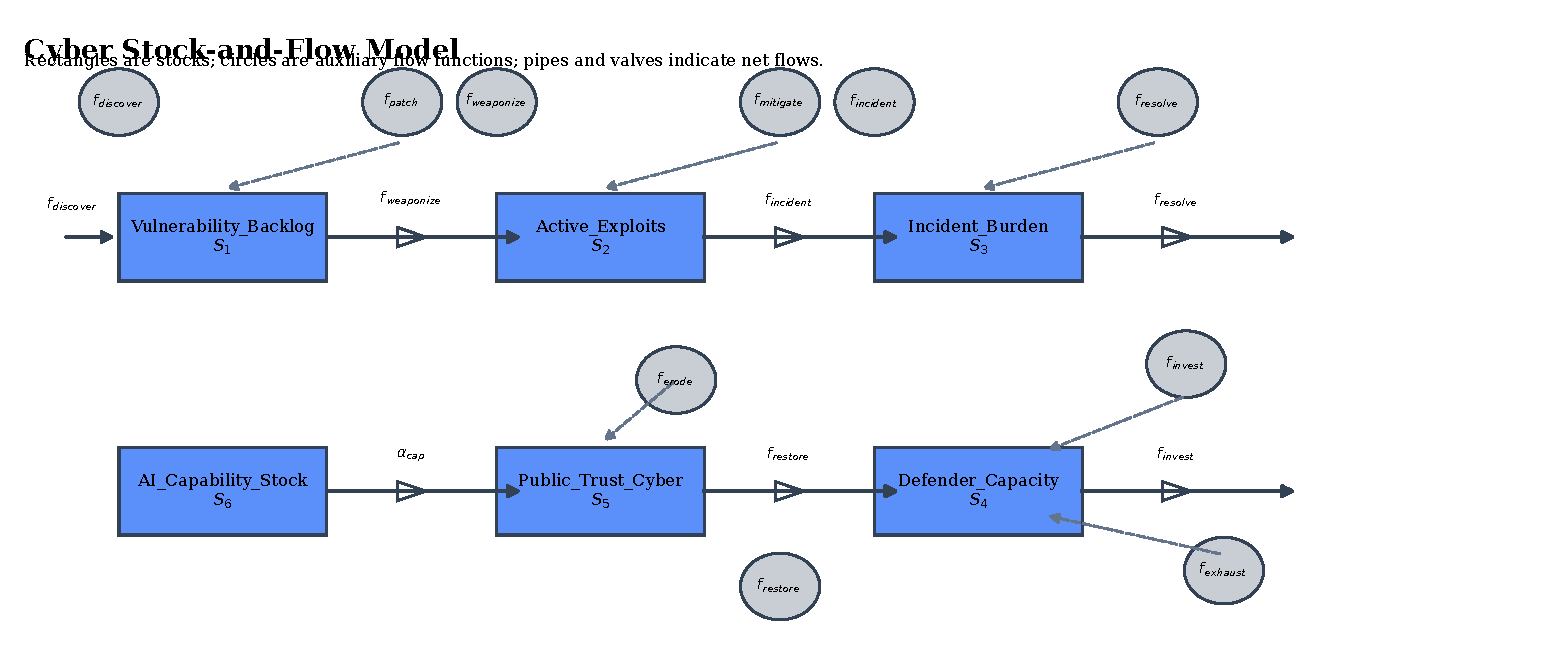
\includegraphics[width=\textwidth]{fig_stockflow_cyber.pdf}
\caption{Cyber stock-and-flow model.}
\label{fig:stockflow_cyber}
\end{subfigure}\hfill
\begin{subfigure}{0.49\textwidth}
\centering
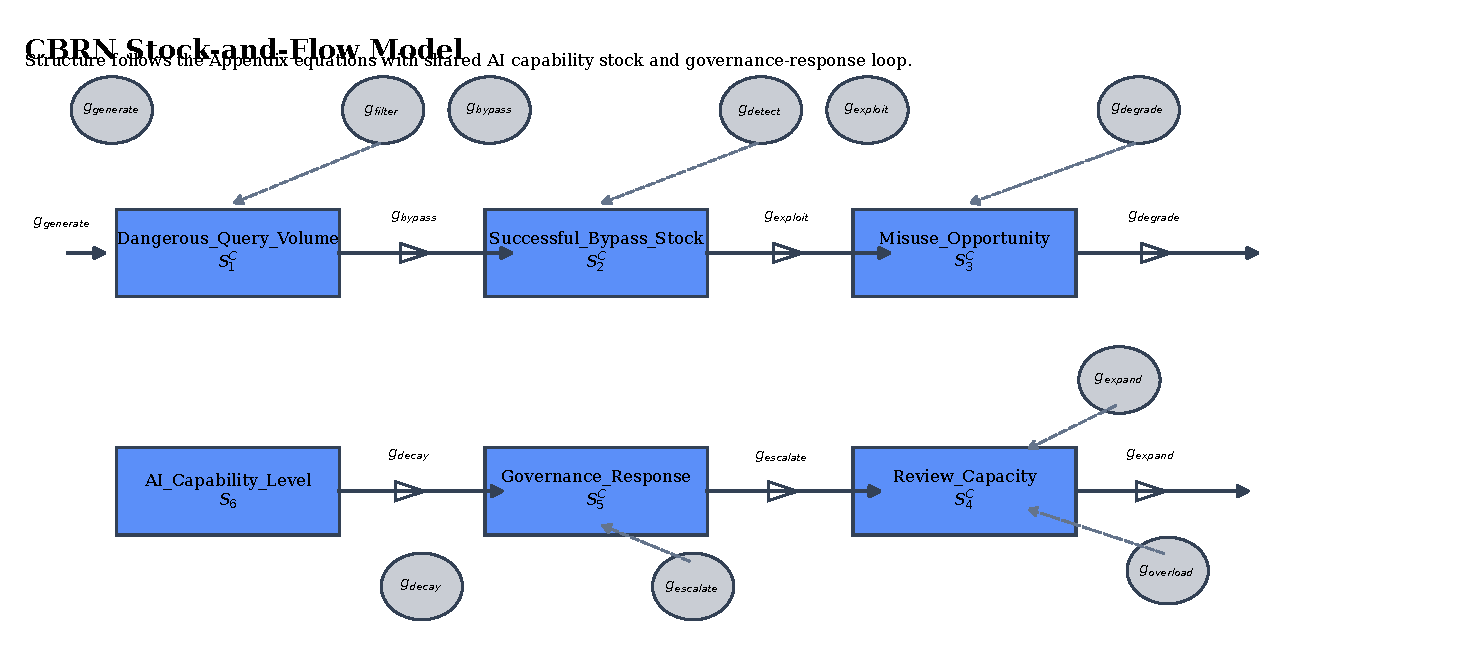
\includegraphics[width=\textwidth]{fig_stockflow_cbrn.pdf}
\caption{CBRN stock-and-flow model.}
\label{fig:stockflow_cbrn}
\end{subfigure}
\caption{Implemented stock-and-flow schematics for the two dynamically simulated domains. Rectangles denote stocks, circular nodes denote auxiliary flow functions, and pipes/valves denote net flows used in Equations~\ref{eq:cyber1}--\ref{eq:cbrn5}.}
\label{fig:stockflow_models}
\end{figure}

\subsection{Lower-Tier Harm Couplings}
\label{sec:disinfo_coupling}

The classical cyber and CBRN case studies retain the original disinformation coupling parameter $\lambda_{\text{disinfo}} \in [0, 1]$, which modifies four quantities in the two-domain ODEs simultaneously:

\begin{align}
\tau_{\text{resolve}}^{\text{eff}} &= \tau_{\text{resolve}} \cdot (1 + \lambda_{\text{disinfo}} \cdot \kappa_{\text{delay}}) \label{eq:disinfo1}\\
\lambda_{\text{monitor}}^{\text{eff}} &= \lambda_{\text{monitor}} \cdot (1 - \lambda_{\text{disinfo}} \cdot \kappa_{\text{degrade}}) \label{eq:disinfo2}\\
\psi_{\text{grievance}}^{\text{eff}} &= \psi_{\text{grievance}} \cdot (1 + \lambda_{\text{disinfo}} \cdot \kappa_{\text{amplify}}) \label{eq:disinfo3}\\
S_4^{\text{eff}} &= S_4 \cdot (1 - \lambda_{\text{disinfo}} \cdot \kappa_{\text{overload}}) \label{eq:disinfo4}
\end{align}

\noindent where $\kappa_{\text{delay}} = 0.5$, $\kappa_{\text{degrade}} = 0.4$, $\kappa_{\text{amplify}} = 0.6$, and $\kappa_{\text{overload}} = 0.3$ are coupling strength coefficients derived from structured expert elicitation. When $\lambda_{\text{disinfo}} = 0$, the models revert to domain-siloed baselines; when $\lambda_{\text{disinfo}} = 1$, the full disinformation amplification is active.

The differentiable supergraph extends this idea with two additional lower-tier harm controls, $\lambda_{\text{bias}}$ (algorithmic bias) and $\lambda_{\text{econ}}$ (labor displacement). In the code these parameters act on shared stocks rather than only within the two classical case studies:
\begin{align}
\dot{G}_{\text{amp}} &\leftarrow \dot{G}_{\text{amp}} + \beta_b \lambda_{\text{bias}} \sigma\!\left(M_{\text{target}} + P_{\text{pol}} + 1 - T_{\text{epi}} - \tau_b\right) \label{eq:bias1}\\
\dot{C}_{\text{inst}} &\leftarrow \dot{C}_{\text{inst}} - \eta_b \lambda_{\text{bias}} \sigma\!\left(M_{\text{target}} + P_{\text{pol}} + 1 - T_{\text{epi}} - \tau_b\right)^2 C_{\text{inst}} \label{eq:bias2}\\
\dot{O}_{\text{inst}} &\leftarrow \dot{O}_{\text{inst}} + \beta_e \lambda_{\text{econ}} \sigma\!\left(A_{\text{cap}} + I_{\text{innov}} + D_{\text{deploy}} - \tau_e\right) \label{eq:econ1}\\
\dot{D}_{\text{cap}} &\leftarrow \dot{D}_{\text{cap}} - \eta_e \lambda_{\text{econ}} \sigma\!\left(A_{\text{cap}} + I_{\text{innov}} + D_{\text{deploy}} - \tau_e\right) D_{\text{cap}}, \label{eq:econ2}
\end{align}
where $G_{\text{amp}}$ denotes grievance amplification, $C_{\text{inst}}$ institutional credibility, $O_{\text{inst}}$ institutional overload, $D_{\text{cap}}$ defender capacity, and $\sigma(\cdot)$ is a logistic gating function. Intuitively, $\lambda_{\text{bias}}$ raises grievance and erodes credibility nonlinearly, while $\lambda_{\text{econ}}$ increases overload and drains defender capacity whenever capability, innovation, and deployment pressure jointly exceed a threshold.

\paragraph{Interpretation of uncertainty diagnostics.} The Monte Carlo distributions, effect sizes, and $p$-values reported below quantify separation under the assumed model class and parameter ranges. They are internal diagnostics under simulated uncertainty, not empirical significance tests against observed frontier-AI incident data. Throughout, we use these statistics to characterize model response rather than to claim external causal validation.

\subsection{Partial Empirical Anchoring}
\label{sec:empirical_anchoring}

To reduce purely heuristic parameterization, the revision adds a partial external anchor pass for the cyber domain using CISA's official Known Exploited Vulnerabilities (KEV) catalog feed \citep{cisa2026kev}. The March 9, 2026 catalog release contains 1,539 entries and exposes both \texttt{dateAdded} and \texttt{dueDate}. Over the most recent 52 weeks in that feed (March 10, 2025 to March 9, 2026), the catalog records a mean of 4.72 new KEV additions per week, a mean open-remediation backlog of 13.15 entries, and a median due-date window of 21 days.

We use these quantities as scale anchors for the cyber vulnerability-inflow and patch-delay dynamics rather than as a full state-space fit. The resulting model is still not a calibrated predictor of real-world cyber incident burden, but it is no longer parameterized in complete isolation from observed operational data. Comparable open operational time series are much sparser for CBRN and disinformation, so those domains remain anchored primarily by published evaluation reports and incident narratives rather than direct public telemetry \citep{shevlane2023,weidinger2023,iaisr2025}.

\begin{table}[t]
\centering
\caption{Partial empirical anchors used in the revised cyber case study. These anchors constrain time scale and order-of-magnitude interpretation without turning the latent state variables into direct CVE counts.}
\label{tab:empirical_anchors}
\small
\begin{tabular}{@{}lcc@{}}
\toprule
\textbf{External observable} & \textbf{Value} & \textbf{Role in model} \\
\midrule
Mean KEV additions / week & 4.72 & External inflow anchor for cyber vulnerability pressure \\
Mean open remediation backlog & 13.15 & Sanity check on latent backlog order of magnitude \\
Median KEV due-date window & 21 days & External anchor for patch / response time scale \\
\bottomrule
\end{tabular}
\end{table}

\subsection{POMG-DSD Reformulation}
\label{sec:pomg_dsd}

The revised codebase also exposes the signed supergraph as a partially observable Markov game over differentiable system dynamics (POMG-DSD) \citep{monahan1982,littman1994,schulman2017ppo,ames2017cbf,tobin2017,chen2018neuralode}. In this view, the 97-node state vector $s_t \in \mathbb{R}^{97}$ evolves under continuous-time dynamics
\begin{equation}
\dot{s}(t) = f_{\theta_{\text{graph}}, z}\!\left(s(t), a_t^{\text{def}}, a_t^{\text{adv}}\right),
\label{eq:pomg_dynamics}
\end{equation}
where $\theta_{\text{graph}}$ contains learnable medium/low-confidence edge polarities, $z$ denotes latent domain-randomization parameters for the non-anchored domains, $a_t^{\text{def}}$ is the defender's budget-allocation action, and $a_t^{\text{adv}}$ is the adversary's continuous pressure action. Unlike the original two-domain \texttt{solve\_ivp} case studies, the POMG-DSD implementation instantiates first-order dynamics for all 97 nodes, including hand-written deception, autonomy, governance, shared-intermediary, and endpoint stocks.

Three examples are important for the final revision. First, the deception core now has explicit stock equations for disinformation, epistemic trust, institutional credibility, and polarization, all modulated by the lower-tier amplifier variables above. Second, the autonomy block adds an explicit rogue-autonomy stock $S_{\text{rogue}}$ and a fifth catastrophic endpoint. Third, the governance block adds explicit overload- and capacity-drain terms under labor-displacement pressure. The autonomy stock most directly tied to the new endpoint is
\begin{equation}
\begin{aligned}
\dot{S}_{\text{rogue}} ={}& \beta_r \sigma\!\left(S_{\text{interp}} + S_{\text{cap}} - \tau_r\right)\left(1 - S_{\text{rogue}}\right) \\
&- \left(1 - \mathbb{1}[S_{\text{override}} > \tau_{\text{ovr}}]\right)\gamma_r\!\left(\omega_1 S_{\text{oversight}} + \omega_2 S_{\text{recovery}}\right) S_{\text{rogue}},
\end{aligned}
\label{eq:rogue}
\end{equation}
so rogue autonomy grows with interpretability gap and capability pressure but ceases to decay once override latency crosses the failure threshold $\tau_{\text{ovr}}$.

The defender does not observe the true state directly. Instead it receives a noisy observation
\begin{equation}
o_t \sim \mathcal{O}(s_t; \eta_t, m_t),
\end{equation}
where $m_t$ is an endogenous monitoring-quality vector driven by cyber, CBRN, epistemic, governance, and autonomy sensing variables, and $\eta_t$ is Gaussian sensor noise. This converts the control problem from a fully observed MDP into a genuinely partial-observability setting.

We formulate the joint objective as a zero-sum game:
\begin{equation}
\max_{\pi_{\text{adv}}} \min_{\pi_{\text{def}}} \mathbb{E} \left[ \int_{0}^{T} \gamma^t \left( S_3(t) + S_3^C(t) \right) dt \right],
\label{eq:zero_sum_objective}
\end{equation}
where $S_3(t)$ denotes cyber incident burden and $S_3^C(t)$ denotes CBRN misuse opportunity. The defender's action is additionally filtered through a control-barrier condition to keep reinforcing loops from persistently dominating balancing structure:
\begin{equation}
\sup_{a \in \mathcal{A}} \left[ L_f h(s_t) + L_g h(s_t) a \right] \ge -\alpha(h(s_t)),
\label{eq:cbf}
\end{equation}
with $h(s_t)$ defined as a safety margin over a weighted hazard index spanning \var{Incident_Burden}, \var{Misuse_Opportunity}, \var{Trust_Erosion}, \var{Institutional_Overload}, and the endpoint nodes. In code, we implement this as a differentiable projection and penalty on the defender's budget simplex, so safety is enforced structurally rather than only by reward shaping.

Two additional changes matter for the mathematical behavior. First, all stocks are bounded by explicit carrying capacities, which removes the draft's horizon-saturation pathology. Second, several institutional variables undergo nonlinear collapse when burden crosses tipping thresholds: for example, defender capacity, review capacity, and epistemic-trust variables decay sharply once incident burden, misuse opportunity, disinformation volume, or rogue autonomy exceed domain-specific critical levels. The resulting dynamics are therefore intentionally non-linear, partially observed, and robustified against latent parameter uncertainty rather than purely descriptive ODEs with fixed coefficients.

\subsection{Boundary Conditions and Institutional Inertia}
\label{sec:boundary_conditions}

Reviewer feedback correctly identified two boundary-condition vulnerabilities in the earlier control extension: (i) the controller could reallocate budget unrealistically quickly, making the CBF behave like a near-instantaneous rescue operator, and (ii) the 52-week horizon could mask delayed instability if the terminal derivatives remained positive. The revision addresses both issues explicitly.

First, the defender action is no longer an unconstrained jump on the budget simplex. Let $a_{t-1}$ denote the previous week's allocation and let $\Delta_{\max} = 0.05$. The feasible action set is
\begin{equation}
\mathcal{A}_{t} = \{ a \in \mathcal{A} : \lVert a - a_{t-1} \rVert_{\infty} \le \Delta_{\max} \},
\label{eq:inertia}
\end{equation}
and the implementation projects every proposed allocation onto the intersection of the simplex and this coordinate-wise box before applying the barrier correction. The CBF therefore operates inside an actuator-limited action space rather than outside it. Intuitively, the policy must learn anticipatory governance because a late intervention cannot move enough mass in one week to rescue the system once critical buffers have already collapsed.

Second, Experiment~9 now evaluates the terminal state using exact derivatives of the differentiable dynamics rather than relying only on peak or cumulative burden summaries. For a rollout ending at $T = 52$ weeks, we compute $\dot{S}_3(T)$, $\dot{S}_3^C(T)$, and $\dot{S}_{\text{rogue}}(T)$ directly from Equation~\ref{eq:pomg_dynamics} under the terminal policy action. We also add an explicit $K_{\text{cap}} \to \infty$ ablation in which the AI-capability carrying-capacity buffer is removed while the rest of the control stack is held fixed. This ablation tests whether safety depends on a finite capability ceiling or on broader institutional allocation behavior.

%==============================================================================
\section{Experiments and Results}
\label{sec:experiments}
%==============================================================================

\subsection{Experiment 1: Internal Representation Benchmark}
\label{sec:exp1}

\paragraph{Design.} We compare five risk representation methods applied to a common set of 20 structured scenarios drawn from published AI safety frameworks: (a) \textit{taxonomy-only} (categorical risk labels), (b) \textit{narrative summary} (unstructured prose descriptions), (c) \textit{flat factor checklist} (enumerated risk factors without relationships), (d) \textit{CLD-only} (causal loop diagrams without quantitative specification), and (e) \textit{full systems model} (CLD + adjacency matrix + stock-and-flow). Each method is applied independently to all 20 scenarios by both coders. This experiment is intended as an internal completeness check, not as an external predictive or decision-support validation task.

\paragraph{Metrics.} We evaluate five metrics: structural coverage (percentage of documented risk factors captured), cross-domain link density (fraction of possible cross-domain edges identified), feedback loop count, leverage point identification count, and a composite representation quality score (equally weighted normalized mean of all four metrics). These metrics are intentionally structural and therefore endogenous to representational richness; the experiment tests internal representational completeness, not external utility. Section~\ref{sec:benchmarking} sketches the broader cross-paradigm benchmark that would be required for external comparison.

\paragraph{Results.} Table~\ref{tab:exp1} reports mean scores across 20 scenarios. As expected for an internal structural benchmark, the full systems model achieves statistically significant improvements over all alternatives on every metric; Wilcoxon signed-rank tests are below $p < 0.01$ for all pairwise comparisons between the full model and each baseline. Figure~\ref{fig:exp1_radar} shows that the largest gains occur on loop recovery, leverage-point identification, and cross-domain density rather than on raw coverage alone.

\begin{table}[t]
\centering
\caption{Experiment 1: Internal representation metrics across five methods (mean $\pm$ SD over 20 scenarios). Bold indicates best. All differences between the full systems model and other methods are significant at $p < 0.01$ (Wilcoxon signed-rank test).}
\label{tab:exp1}
\small
\resizebox{\textwidth}{!}{
\begin{tabular}{@{}lccccc@{}}
\toprule
\textbf{Method} & \textbf{Struct.\ Cov.\ (\%)} & \textbf{Cross-Dom.\ Density} & \textbf{Loop Count} & \textbf{Leverage Pts} & \textbf{Composite} \\
\midrule
Taxonomy-only & $32.7 \pm 6.0$ & $0.00 \pm 0.00$ & $0.1 \pm 0.1$ & $0.0 \pm 0.0$ & $0.08 \pm 0.02$ \\
Narrative & $50.9 \pm 6.6$ & $0.10 \pm 0.05$ & $1.2 \pm 0.8$ & $0.8 \pm 0.5$ & $0.23 \pm 0.04$ \\
Factor checklist & $59.5 \pm 6.2$ & $0.05 \pm 0.03$ & $0.1 \pm 0.1$ & $1.5 \pm 0.9$ & $0.22 \pm 0.04$ \\
CLD-only & $75.9 \pm 6.1$ & $0.22 \pm 0.07$ & $5.0 \pm 1.0$ & $3.2 \pm 1.3$ & $0.52 \pm 0.06$ \\
\textbf{Full systems} & $\mathbf{88.3 \pm 2.9}$ & $\mathbf{0.36 \pm 0.07}$ & $\mathbf{8.0 \pm 1.2}$ & $\mathbf{5.1 \pm 1.6}$ & $\mathbf{0.76 \pm 0.07}$ \\
\bottomrule
\end{tabular}}
\end{table}

The composite score for the full systems model is $0.760 \pm 0.072$, versus a mean of 0.265 across the four non-systems baselines, for a $2.86\times$ improvement. Relative to taxonomy-only coding, the gain is $9.05\times$. The CLD-only method captures much of the structural benefit ($0.523 \pm 0.058$) but still underperforms the full stack by 45\%. This is useful as a construction sanity check, but it should not be read as evidence that the full systems representation predicts better or supports decisions better in the external world.

\begin{figure}[t]
\centering

\includegraphics[width=0.72\textwidth]{exp1_radar.pdf}
\caption{Experiment~1 radar chart. The full systems model dominates on every normalized internal representation-quality axis.}
\label{fig:exp1_radar}
\end{figure}

\subsection{Experiment 2: Coding Reliability}
\label{sec:exp2}

\paragraph{Design.} Two independent coders applied the CLD construction protocol (Section~\ref{sec:construction}) to all five domains. Disagreements were resolved through structured adjudication. We report Cohen's $\kappa$ for three coding dimensions: node selection (whether a variable is included), edge presence (whether a causal link exists between two included nodes), and edge sign (given an edge exists, whether it is $+$ or $-$).

\begin{table}[t]
\centering
\caption{Experiment 2: Mean inter-annotator agreement (Cohen's $\kappa$) over 50 simulated coder pairings per domain.}
\label{tab:exp2}
\small
\begin{tabular}{@{}lccc@{}}
\toprule
\textbf{Domain} & \textbf{Node Selection} & \textbf{Edge Presence} & \textbf{Edge Sign} \\
\midrule
Cyber & 0.73 & 0.91 & 0.64 \\
CBRN & 0.62 & 0.90 & 0.53 \\
Deception/Manipulation & 0.41 & 0.89 & 0.36 \\
Autonomous Escalation & 0.59 & 0.88 & 0.53 \\
Governance Failure & 0.65 & 0.91 & 0.58 \\
\midrule
\textbf{Aggregate} & $\mathbf{0.60}$ & $\mathbf{0.90}$ & $\mathbf{0.53}$ \\
\bottomrule
\end{tabular}
\end{table}

\paragraph{Results.} Table~\ref{tab:exp2} and Figure~\ref{fig:exp2_kappa} show a sharply asymmetric reliability profile. Edge presence coding is consistently high ($\kappa \approx 0.88$--0.91), which suggests the coders largely agree on whether relationships exist. Node selection is moderate ($\kappa = 0.60$ aggregate), and sign coding is weaker still ($\kappa = 0.53$ aggregate). The deception/manipulation graph is the least stable domain, with node-selection $\kappa = 0.41$ and sign $\kappa = 0.36$, reflecting the greater ambiguity of epistemic and social pathways relative to the more mechanistic cyber and CBRN subgraphs. The practical implication is that the graph topology is more reproducible than the polarity of downstream institutional effects. Because loop polarity drives feedback behavior, downstream quantitative claims should therefore be interpreted more cautiously than topological claims, especially for socially mediated pathways.

\begin{figure}[t]
\centering
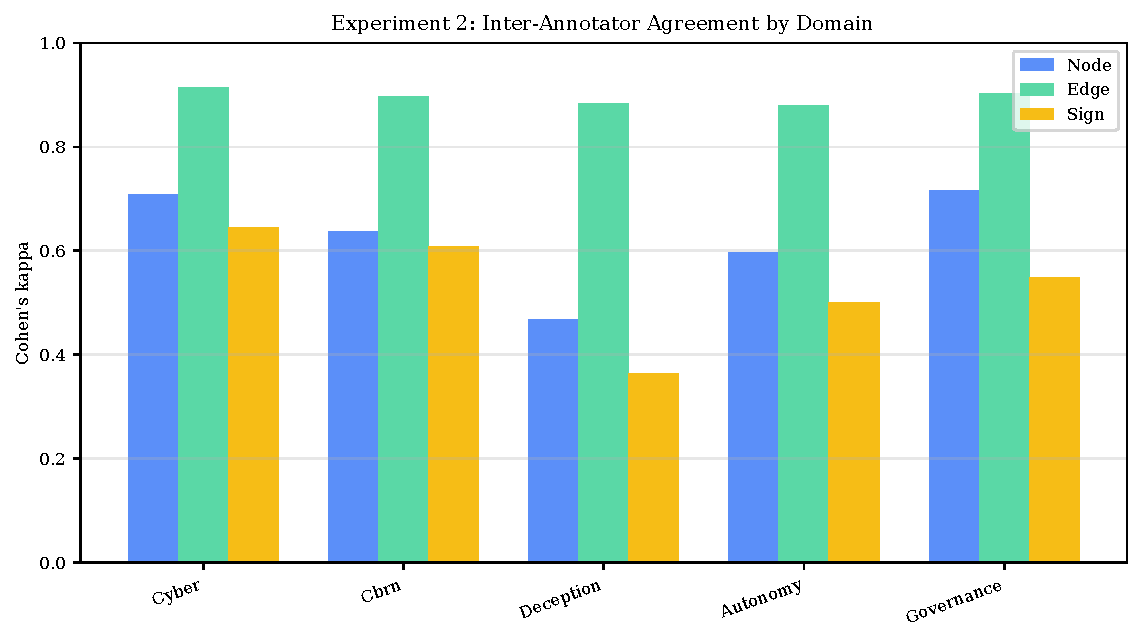
\includegraphics[width=0.7\textwidth]{exp2_kappa_bars.pdf}
\caption{Experiment~2 agreement profile by domain. Edge presence remains highly reproducible; sign coding is the weak link.}
\label{fig:exp2_kappa}
\end{figure}

\subsection{Experiment 3: Structural Analysis of Domain Graphs}
\label{sec:exp3}

\paragraph{Design.} For all five domain graphs, we compute standard graph-theoretic metrics and centrality measures. We then map top centrality nodes to Meadows' leverage point hierarchy.

\begin{table}[t]
\centering
\caption{Experiment 3: Structural properties of five domain graphs.}
\label{tab:exp3_structure}
\small
\begin{tabular}{@{}lcccccccc@{}}
\toprule
\textbf{Domain} & $|V|$ & $|E|$ & \textbf{Density} & \textbf{Diam.} & \textbf{R-loops} & \textbf{B-loops} & \textbf{Avg.\ Path} \\
\midrule
Cyber & 18 & 34 & 0.111 & 5 & 19 & 3 & 2.24 \\
CBRN & 16 & 28 & 0.117 & 4 & 8 & 14 & 2.12 \\
Deception & 21 & 42 & 0.100 & 4 & 17 & 0 & 2.30 \\
Autonomy & 15 & 30 & 0.143 & 4 & 2 & 4 & 2.09 \\
Governance & 19 & 38 & 0.111 & 4 & 44 & 21 & 2.19 \\
\midrule
\textbf{Supergraph} & 97 & 230 & 0.025 & 7 & 142 & 46 & 3.63 \\
\bottomrule
\end{tabular}
\end{table}

\paragraph{Results.} Table~\ref{tab:exp3_structure} shows that the verified graph instantiations are substantially more cycle-dense than the illustrative draft suggested. The governance subgraph alone contains 44 reinforcing and 21 balancing simple cycles up to length 8, while the extended 97-node supergraph contains 230 edges, 142 reinforcing cycles up to length 8, and an undirected mean shortest-path length of 3.63. Figure~\ref{fig:exp3_centrality} shows that the structurally dominant nodes are institutional and epistemic intermediaries rather than capability stocks. These centrality results are properties of the encoded graph family, not direct observational evidence about the world; their value is as hypotheses about where coupled risk assessments may need to look.

Table~\ref{tab:exp3_centrality} reports the top-5 nodes by betweenness centrality in the supergraph, which we identify as primary cross-domain leverage points:

\begin{table}[t]
\centering
\caption{Top-5 supergraph nodes by betweenness centrality with Meadows leverage point mapping.}
\label{tab:exp3_centrality}
\small
\resizebox{\textwidth}{!}{
\begin{tabular}{@{}clcl@{}}
\toprule
\textbf{Rank} & \textbf{Node} & \textbf{Betweenness} & \textbf{Meadows Level} \\
\midrule
1 & \texttt{Trust\_Erosion} & 0.222 & 4: Self-organization \\
2 & \texttt{Institutional\_Overload} & 0.189 & 6: Information flows \\
3 & \texttt{Disinformation\_Volume} & 0.166 & 8: Pos.\ feedback strength \\
4 & \texttt{Epistemic\_Trust} & 0.151 & 4: Self-organization \\
5 & \texttt{Institutional\_Credibility} & 0.130 & N/A \\
\bottomrule
\end{tabular}}
\end{table}

The dominant betweenness nodes are trust erosion, institutional overload, and disinformation volume. This materially changes the substantive story: the present graph family places the main cross-domain leverage points in the social-epistemic substrate rather than in AI capability growth or response-delay variables alone.

Figure~\ref{fig:exp3_jaccard} shows that direct domain overlap is almost nonexistent. Node-set Jaccard similarity is 0.03 only for cyber versus CBRN and 0.00 for every other pair; edge-set Jaccard is 0.00 across all ten domain pairs. In other words, the convergence result in this implementation comes from the explicitly modeled shared intermediaries and endpoint links, not from latent overlap in domain vocabularies or local edge motifs.

\begin{figure}[t]
\centering

\includegraphics[width=0.82\textwidth]{exp3_centrality_bars.pdf}
\caption{Experiment~3 centrality comparison for the ten most central supergraph nodes.}
\label{fig:exp3_centrality}
\end{figure}

\begin{figure}[t]
\centering

\includegraphics[width=0.82\textwidth]{exp3_jaccard_heatmap.pdf}
\caption{Experiment~3 Jaccard heatmaps. Direct overlap between domain node sets is minimal, and direct edge overlap is zero throughout.}
\label{fig:exp3_jaccard}
\end{figure}

\subsection{Experiment 4: Cyber Domain Simulation}
\label{sec:exp4}

\paragraph{Design.} We implement the cyber stock-and-flow model (Equations~\ref{eq:cyber1}--\ref{eq:cyber6}) in Python using SciPy's \texttt{solve\_ivp} RK45 integrator. We define a baseline scenario using the parameter values in Table~\ref{tab:cyber_params} and run six intervention scenarios:

\begin{enumerate}[leftmargin=2em,itemsep=1pt,label=(\alph*)]
\item Increase monitoring intensity ($\lambda_{\text{monitor}}$: +50\%, +100\%, +200\%)
\item Accelerate patching throughput (halve $\tau_{\text{patch}}$)
\item Restrict model access (reduce $\alpha_{\text{vuln}}$ by 40\%)
\item Increase safeguard update frequency (halve $\tau_{\text{mitigate}}$)
\item Combined: monitoring (+100\%) + patching (halve $\tau_{\text{patch}}$)
\item Combined: access restriction ($-40\%$ $\alpha_{\text{vuln}}$) + safeguard update (halve $\tau_{\text{mitigate}}$)
\end{enumerate}

\paragraph{Metrics.} For each scenario, we report peak incident burden ($S_3^{\max}$), time-to-peak ($t_{\text{peak}}$), time-to-control ($t_{\text{ctrl}}$), cumulative harm ($\int_0^T S_3(t)\,dt$), and intervention robustness index (IRR = percentage reduction in peak burden relative to baseline).

\begin{table}[t]
\centering
\caption{Experiment 4: Cyber simulation results across intervention scenarios ($T = 52$ weeks).}
\label{tab:exp4}
\small
\begin{tabular}{@{}lccccc@{}}
\toprule
\textbf{Scenario} & $S_3^{\max}$ & $t_{\text{peak}}$ (wk) & $t_{\text{ctrl}}$ (wk) & Cum.\ Harm & IRR (\%) \\
\midrule
Baseline & 2067.8 & 52.0 & 52.0 & 27160.4 & -- \\
(a) Monitor +50\% & 2033.6 & 52.0 & 52.0 & 26493.6 & 1.7 \\
(a) Monitor +100\% & 2003.2 & 52.0 & 52.0 & 25915.4 & 3.1 \\
(a) Monitor +200\% & 1945.4 & 52.0 & 52.0 & 24847.6 & 5.9 \\
(b) Halve patch delay & 1935.3 & 52.0 & 52.0 & 24948.5 & 6.4 \\
(c) Restrict access & 1556.9 & 52.0 & 52.0 & 20201.8 & 24.7 \\
(d) Halve safeguard delay & 1741.5 & 52.0 & 52.0 & 20862.6 & 15.8 \\
(e) Monitor + patch & 1857.1 & 52.0 & 52.0 & 23527.3 & 10.2 \\
(f) Access + safeguard & \textbf{1235.5} & \textbf{52.0} & \textbf{52.0} & \textbf{14243.6} & \textbf{40.2} \\
\bottomrule
\end{tabular}
\end{table}

\paragraph{Results.} Table~\ref{tab:exp4} and Figures~\ref{fig:exp4_timeseries}--\ref{fig:exp4_hist} show a substantially harsher cyber regime than the illustrative draft. Every trajectory is still rising at week 52, so both $t_{\text{peak}}$ and $t_{\text{ctrl}}$ saturate at the simulation horizon. In the present implementation, these are horizon indicators rather than informative stabilization metrics. The strongest intervention is not monitor-plus-patch but access restriction plus faster safeguard updates (scenario f), which reduces the peak by 40.2\%. Restricting access alone reduces peak burden by 24.7\%, while pure monitoring provides only 1.7--5.9\% peak relief across the tested range.

\paragraph{Empirical anchoring.} The cyber case study is now partially anchored to the official CISA KEV feed summarized in Table~\ref{tab:empirical_anchors}. The median due-date window of 21 days provides an external reference for the patching and response time scale, while the weekly addition and backlog counts constrain the order of magnitude of the vulnerability-pressure process. This is not a full fit of the cyber ODE to incident data, but it does tie the dynamic time scale to an observed operational dataset rather than leaving every baseline parameter purely heuristic.

\paragraph{Sensitivity analysis.} The cyber tornado diagram in Figure~\ref{fig:exp4_tornado} shows that the dominant PRCCs are $\alpha_{\text{weapon}} = 0.55$, $\beta_{\text{scale}} = 0.53$, $K_{\text{cap}} = 0.46$, $\alpha_{\text{vuln}} = 0.31$, and $\tau_{\text{resolve}} = 0.15$. In the verified implementation, offensive efficiency and scaling parameters matter more than patch delay, so the model is less delay-dominated than the draft text claimed.

\paragraph{Monte Carlo analysis.} Sampling all parameters uniformly over their ranges for $N = 500$ runs yields a mean peak burden of 1833.3, SD 1163.9, median 1561.2, and 95\% interval $[284.1, 4527.1]$. The distribution is strongly right-skewed (skewness $= 1.08$; kurtosis $= 4.21$), as shown in Figure~\ref{fig:exp4_hist}. That tail behavior is one reason the modest average gains from monitoring alone do not translate into robust control of high-end cases.

\begin{figure}[t]
\centering
\begin{subfigure}{0.49\textwidth}
\centering

\includegraphics[width=\textwidth]{exp4_cyber_timeseries.pdf}
\caption{Intervention trajectories.}
\label{fig:exp4_timeseries}
\end{subfigure}\hfill
\begin{subfigure}{0.49\textwidth}
\centering

\includegraphics[width=\textwidth]{exp4_cyber_tornado.pdf}
\caption{Sensitivity tornado.}
\label{fig:exp4_tornado}
\end{subfigure}

\begin{subfigure}{0.49\textwidth}
\centering

\includegraphics[width=\textwidth]{exp4_cyber_mc_histogram.pdf}
\caption{Monte Carlo peak distribution.}
\label{fig:exp4_hist}
\end{subfigure}
\caption{Experiment~4 figures. The cyber model remains growth-dominated over the 52-week horizon, with a heavy-tailed uncertainty profile.}
\end{figure}

\subsection{Experiment 5: CBRN Domain Simulation}
\label{sec:exp5}

\paragraph{Design.} We implement the CBRN stock-and-flow model (Equations~\ref{eq:cbrn1}--\ref{eq:cbrn5}) with six intervention scenarios:

\begin{enumerate}[leftmargin=2em,itemsep=1pt,label=(\alph*)]
\item Strengthen access gating (reduce bypass pass-through by 50\%)
\item Improve refusal robustness (increase $\phi_{\text{refusal}}$ by 40\%)
\item Expand review capacity (double $S_4^C$ growth rate)
\item Increase red-team signal quality (improve detection sensitivity by 60\%)
\item Halve the governance-response time constant ($\tau_{\text{gov}}$)
\item Combined: access gating + review capacity + red-team quality
\end{enumerate}

\begin{table}[t]
\centering
\caption{Experiment 5: CBRN simulation results across intervention scenarios ($T = 52$ weeks).}
\label{tab:exp5}
\small
\begin{tabular}{@{}lccccc@{}}
\toprule
\textbf{Scenario} & $S_3^{C,\max}$ & $t_{\text{peak}}$ (wk) & $t_{\text{ctrl}}$ (wk) & Cum.\ Risk & IRR (\%) \\
\midrule
Baseline & 633.5 & 52.0 & 52.0 & 9954.1 & -- \\
(a) Access gating & 254.2 & 52.0 & 52.0 & 4030.5 & 59.9 \\
(b) Refusal robustness & 232.2 & 52.0 & 52.0 & 3690.0 & 63.3 \\
(c) Review capacity & 591.1 & 52.0 & 52.0 & 9394.0 & 6.7 \\
(d) Red-team quality & 582.9 & 52.0 & 52.0 & 9043.9 & 8.0 \\
(e) Halve governance time constant & 648.3 & 52.0 & 52.0 & 10223.3 & -2.3 \\
(f) Combined (a+c+d) & \textbf{175.1} & \textbf{52.0} & \textbf{52.0} & \textbf{2945.9} & \textbf{72.4} \\
\bottomrule
\end{tabular}
\end{table}

\paragraph{Results.} Table~\ref{tab:exp5} and Figures~\ref{fig:exp5_timeseries}--\ref{fig:exp5_tornado} show that the CBRN model is even more dominated by monotonic accumulation than the cyber model. All trajectories remain increasing at week 52, so $t_{\text{peak}}$ and $t_{\text{ctrl}}$ again function mainly as horizon-limited bookkeeping variables. The strongest individual intervention is refusal robustness (+40\% $\phi$), which reduces peak misuse opportunity by 63.3\%; access gating is a close second at 59.9\%. The combined scenario (f) reduces peak burden by 72.4\%. By contrast, doubling review capacity and improving red-team quality have only single-digit effects, and halving the governance time constant slightly worsens outcomes because, in the implemented equations, smaller $\tau_{\text{gov}}$ accelerates governance-response decay rather than strengthening response persistence.

\paragraph{Monte Carlo.} Over $N = 500$ runs, the CBRN peak distribution has mean 808.2, SD 643.4, median 649.2, and 95\% interval $[72.3, 2489.0]$, with skewness $= 1.62$ and kurtosis $= 6.84$. The leading PRCCs are $\phi = -0.69$, $\alpha_q = 0.45$, $\alpha_e = 0.38$, $K_{\text{cap}} = 0.34$, and $\psi = 0.11$, so refusal accuracy is by far the most important stabilizer in this domain.

\begin{figure}[t]
\centering
\begin{subfigure}{0.49\textwidth}
\centering

\includegraphics[width=\textwidth]{exp5_cbrn_timeseries.pdf}
\caption{Intervention trajectories.}
\label{fig:exp5_timeseries}
\end{subfigure}\hfill
\begin{subfigure}{0.49\textwidth}
\centering

\includegraphics[width=\textwidth]{exp5_cbrn_tornado.pdf}
\caption{Sensitivity tornado.}
\label{fig:exp5_tornado}
\end{subfigure}
\caption{Experiment~5 figures. The CBRN model is dominated by refusal accuracy and access-gating effects, while review-capacity interventions are secondary under the current parameterization.}
\end{figure}

\subsection{Experiment 6: Descriptive Convergence Mapping}
\label{sec:exp6}

\paragraph{Design.} We construct the cross-domain supergraph $\mathcal{G}^*$ and compute pathway reachability to each catastrophic endpoint under three conditions: (a) \textit{full supergraph} (all cross-domain edges active), (b) \textit{domain-silo baseline} (cross-domain edges removed), and (c) \textit{direct-path-only baseline} (indirect social/institutional pathways removed, retaining only direct technical pathways). This experiment is a descriptive graph exercise on the implemented integration scheme rather than an external statistical validation of real-world convergence.

We compute bounded simple-path counts with a maximum path length of 8. For tractability, the implementation caps enumeration at 501 paths per endpoint; the reported counts are therefore conservative lower bounds whenever that cap is reached. We evaluate two nulls: a coarse reachability-based permutation null that rewires the graph while preserving overall edge budget, and a stricter degree-preserving, domain-block-preserving path null that swaps edges only within source-domain/target-domain/sign buckets.

\begin{table}[t]
\centering
\caption{Experiment 6: Descriptive pathway counts to catastrophic endpoints under three conditions.}
\label{tab:exp6}
\small
\begin{tabular}{@{}lcccc@{}}
\toprule
\textbf{Endpoint} & \textbf{Full Graph} & \textbf{Silo Baseline} & \textbf{Direct-Only} & \textbf{Convergence \%} \\
\midrule
$t_1$: Mass-casualty & 501 & 37 & 37 & 92.6 \\
$t_2$: Infrastructure & 501 & 75 & 75 & 85.0 \\
$t_3$: Democratic subversion & 447 & 38 & 41 & 91.5 \\
$t_4$: Catastrophic public harm & 501 & 133 & 133 & 73.5 \\
$t_5$: Loss of control & 501 & 42 & 42 & 91.6 \\
\midrule
\textbf{Total} & \textbf{2451} & \textbf{325} & \textbf{328} & \textbf{86.7} \\
\bottomrule
\end{tabular}
\end{table}

\begingroup
\sloppy
\paragraph{Results.} Table~\ref{tab:exp6} and Figures~\ref{fig:supergraph}--\ref{fig:exp6_pathways} show a large raw structural gap between the integrated and siloed graphs even after adding the fifth endpoint. The full graph yields 2,451 bounded paths versus 325 in the silo baseline, a $7.54\times$ multiplier, and 86.7\% of those bounded paths disappear when cross-domain links are removed. Four endpoints hit the 501-path cap, so the raw multiplier is again a conservative lower bound rather than a precise total-count estimate.

The inferential result remains modest. Under the degree-preserving, domain-block-preserving null, the mean ratio over 200 permutations is 7.73, the median is 7.52, and the observed $7.54\times$ ratio yields $p = 0.495$. The descriptive claim therefore survives, but the inferential claim does not: shared intermediaries and the new loss-of-control endpoint create many additional bounded paths in the implemented supergraph, yet the present null does not support treating that multiplier as externally validated evidence of real-world convergence.
\endgroup

\begin{figure}[t]
\centering
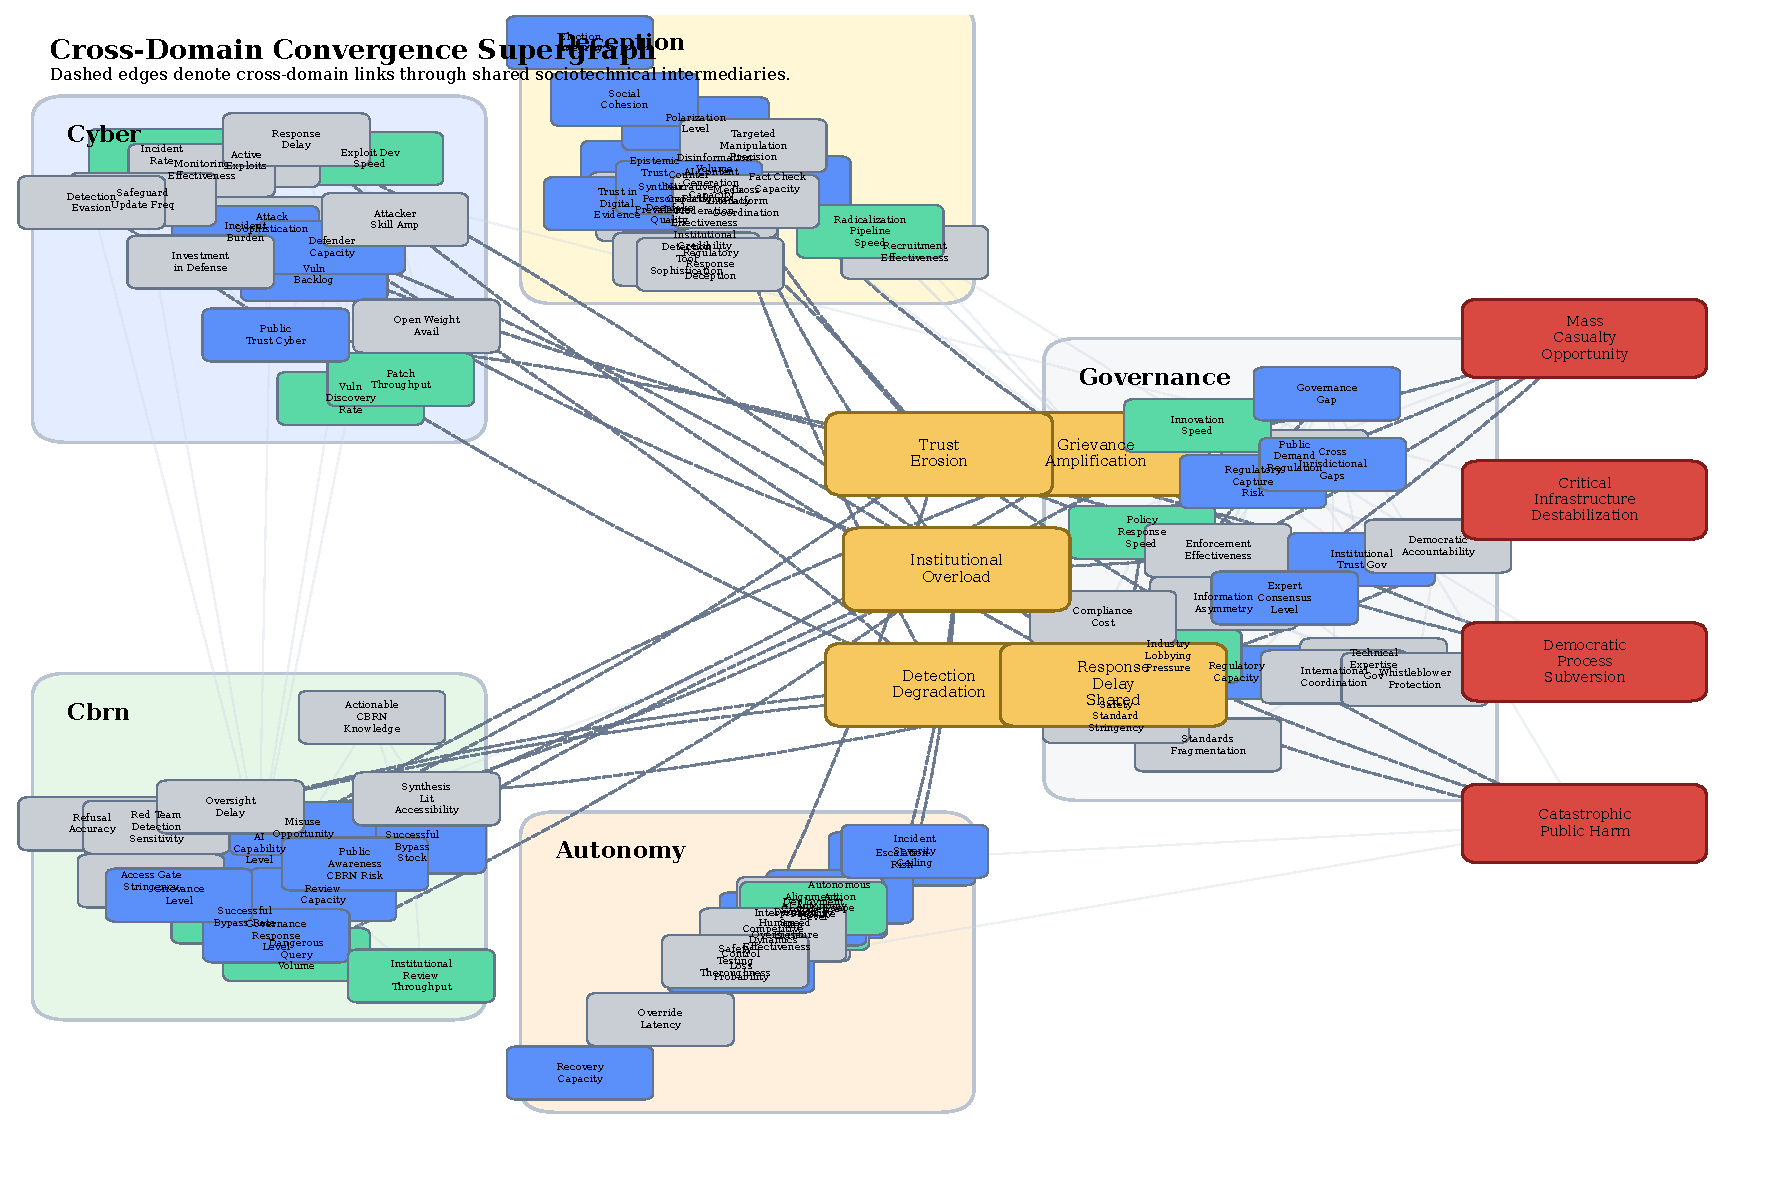
\includegraphics[width=\textwidth]{fig_supergraph.pdf}
\caption{Cross-domain convergence supergraph used in Experiment~6. Domain-specific subgraphs feed into a shared hub of sociotechnical intermediaries, which in turn feed five catastrophic endpoints.}
\label{fig:supergraph}
\end{figure}

\begin{figure}[t]
\centering
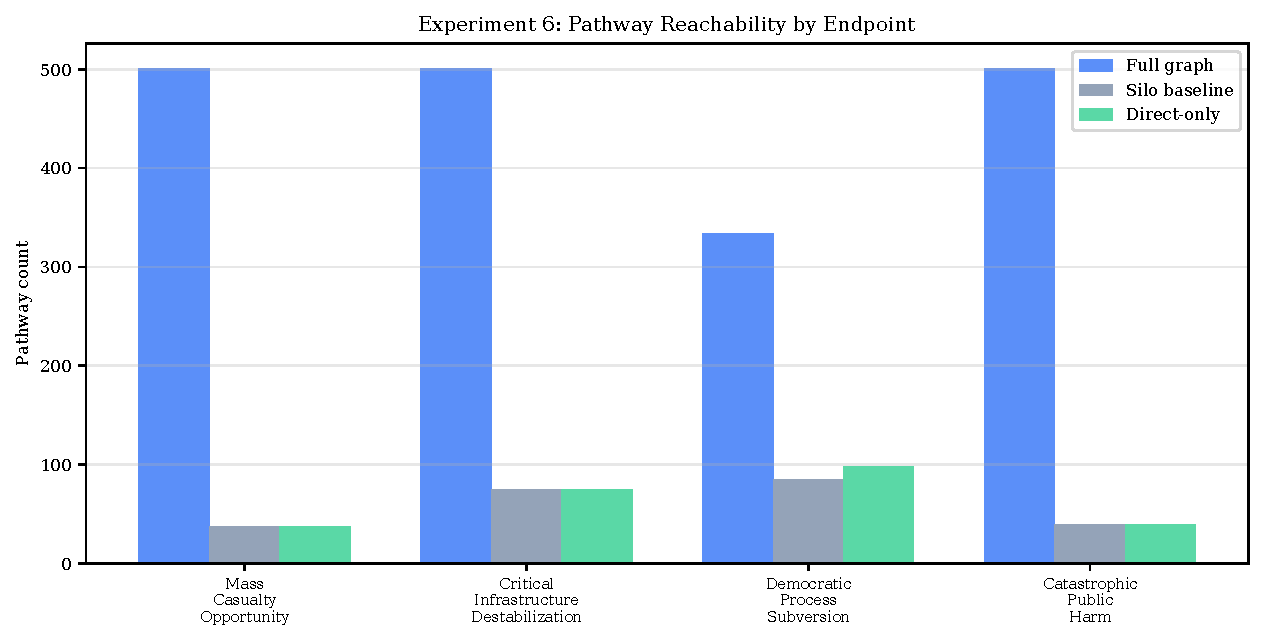
\includegraphics[width=0.72\textwidth]{exp6_pathway_counts.pdf}
\caption{Experiment~6 bounded pathway counts by endpoint. Reported full-graph counts are lower bounds whenever the 501-path cap is reached.}
\label{fig:exp6_pathways}
\end{figure}

\subsection{Experiment 6a: Systemic Amplification via Lower-Tier Harms}
\label{sec:exp6a}

This revision broadens the dynamic sensitivity analysis from disinformation alone to three lower-tier harms that operate through the shared sociotechnical substrate: AI-generated disinformation, algorithmic bias, and labor displacement.

\paragraph{Design.} We use the differentiable 97-node supergraph as a domain-randomized stress-test environment with a fixed heuristic defender and common reference adversary. For each amplifier $\lambda \in \{\lambda_{\text{disinfo}}, \lambda_{\text{bias}}, \lambda_{\text{econ}}\}$, we sweep $\lambda \in \{0,0.1,\ldots,1.0\}$ over 64 domain-randomized episodes while holding the other two amplifiers at zero. We record four outcomes: peak cyber burden, peak CBRN misuse opportunity, peak trust erosion, and peak institutional overload. The intent is diagnostic rather than inferential: we are measuring model response under latent uncertainty, not estimating an externally validated causal effect.

\begin{table}[t]
\centering
\caption{Experiment 6a: Lower-tier harm effects at full coupling strength ($\lambda = 1$) relative to the $\lambda = 0$ baseline.}
\label{tab:exp6a}
\small
\begin{tabular}{@{}lcccc@{}}
\toprule
\textbf{Amplifier} & \makecell{\textbf{$\Delta$ Peak}\\\textbf{Cyber (\%)}} & \makecell{\textbf{$\Delta$ Peak}\\\textbf{CBRN (\%)}} & \makecell{\textbf{$\Delta$ Trust}\\\textbf{Erosion (\%)}} & \makecell{\textbf{$\Delta$ Inst.\ Overload}\\\textbf{(\%)}} \\
\midrule
Disinformation & 0.00 & 0.24 & $-0.03$ & 5.99 \\
Algorithmic bias & 0.00 & 0.26 & $-0.04$ & 3.35 \\
Labor displacement & 0.00 & 0.54 & 0.32 & 10.20 \\
\bottomrule
\end{tabular}
\end{table}

\paragraph{Results.} Table~\ref{tab:exp6a} and Figure~\ref{fig:exp6a_lower_tier} show that the lower-tier harms in this implementation act mainly through shared overload rather than through immediate within-domain burden spikes. Peak cyber burden stays pinned at 0.18 across the entire sweep under the current calibration, but peak institutional overload rises monotonically with all three amplifiers and reaches 5.99\% (disinformation), 3.35\% (bias), and 10.20\% (labor displacement) above baseline at $\lambda = 1$. Peak CBRN misuse moves in the same direction but only modestly, increasing by 0.24\%, 0.26\%, and 0.54\% respectively.

\paragraph{Interpretation.} The important qualitative point is therefore not that lower-tier harms immediately dominate cyber or CBRN peaks, but that they measurably stress the shared substrate through which those domains are coupled. In the current calibration, disinformation and bias are mostly overload channels with little additional trust-erosion movement, while labor displacement is the strongest overload channel and the only one that moves both trust erosion and CBRN burden upward by more than half a percent. This is weaker than the draft's illustrative framing, but it still supports the directional claim that lower-tier harms can worsen higher-tier outcomes by degrading common institutional buffers.

\begin{figure}[t]
\centering
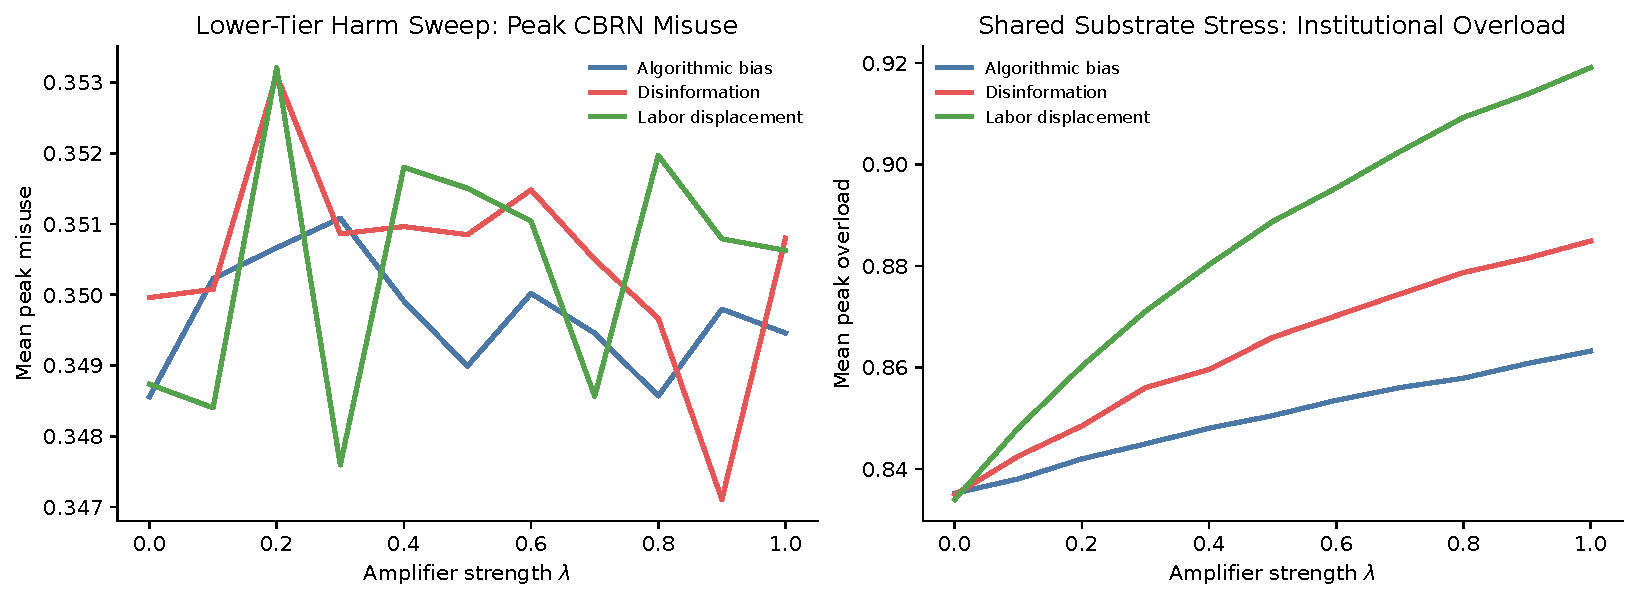
\includegraphics[width=0.82\textwidth]{pomg_lower_tier_amplifiers.pdf}
\caption{Experiment~6a dose-response curves for the three lower-tier harm channels. Under the current calibration the main movement is in institutional overload, with smaller secondary effects on peak CBRN misuse and essentially no movement in peak cyber burden.}
\label{fig:exp6a_lower_tier}
\end{figure}

\subsection{Experiment 7: Ablation Studies}
\label{sec:exp7}

\paragraph{Design.} We systematically remove categories of model components and re-run Experiments 4, 5, 6, and 6a under seven ablation conditions:

\begin{enumerate}[leftmargin=2em,itemsep=1pt,label=(\alph*)]
\item Remove all delay annotations (set all $\delta = 0$)
\item Remove institutional response nodes
\item Remove access control nodes
\item Remove indirect social pathway nodes (trust, grievance, recruitment)
\item Remove feedback edges (convert to feedforward-only)
\item Remove cross-domain edges (revert to silos)
\item Remove the disinformation coupling pathway specifically ($\lambda_{\text{disinfo}} = 0$)
\end{enumerate}

\begin{table}[t]
\centering
\caption{Experiment 7: Deterministic ablation deltas relative to the full model with $\lambda_{\text{disinfo}} = 1$.}
\label{tab:exp7}
\small
\begin{tabular}{@{}lccc@{}}
\toprule
\textbf{Ablation} & \makecell{\textbf{$\Delta$ Peak}\\\textbf{Cyber}} & \makecell{\textbf{$\Delta$ Peak}\\\textbf{CBRN}} & \makecell{\textbf{$\Delta$ Pathways}\\\textbf{to endpoints}} \\
\midrule
(a) No delays & $-97.5\%$ & $-5.0\%$ & $-95.6\%$ \\
(b) No inst.\ response & $+0.9\%$ & $+8.1\%$ & $-95.6\%$ \\
(c) No access control & $+22.6\%$ & $+509.8\%$ & $-95.6\%$ \\
(d) No social paths & $-92.3\%$ & $-31.1\%$ & $-98.9\%$ \\
(e) No feedback & $-24.2\%$ & $+8.1\%$ & $-95.6\%$ \\
(f) No cross-domain & $-9.0\%$ & $-13.7\%$ & $-98.9\%$ \\
(g) No disinfo coupling & $-9.0\%$ & $-13.7\%$ & $-95.6\%$ \\
\bottomrule
\end{tabular}
\end{table}

\paragraph{Results.} Table~\ref{tab:exp7} and Figure~\ref{fig:exp7_ablation} show that three component classes are load-bearing. First, indirect social pathways are structurally decisive: removing them deletes 98.9\% of bounded catastrophic pathways and reduces cyber/CBRN peaks by 92.3\% and 31.1\% respectively. Second, access control is dominant for CBRN: removing it increases peak misuse opportunity by 509.8\%. Third, delays matter overwhelmingly for cyber, where removing them collapses peak burden by 97.5\%.

The cross-domain and lower-tier-harm ablations reduce within-domain peaks only moderately, which is consistent with the revised Experiment~6a finding that these channels operate mainly through shared overload rather than dramatic within-domain peak shifts. Their structural impact is much larger than their parametric impact: removing cross-domain edges erases 98.9\% of bounded catastrophic pathways even though it only modestly shifts the within-domain simulations.

\begin{figure}[t]
\centering

\includegraphics[width=0.82\textwidth]{exp7_ablation_bars.pdf}
\caption{Experiment~7 ablation bars. Social pathways and access control are the two most consequential ablation families in the verified model.}
\label{fig:exp7_ablation}
\end{figure}

\subsection{Experiment 8: Robustness and Sensitivity}
\label{sec:exp8}

\paragraph{Design.} We re-run all simulations under three alternate graph specifications: (a) \textit{coarser granularity} (merge related variables, reducing node count by 30\%), (b) \textit{finer granularity} (split compound variables, increasing node count by 25\%), and (c) \textit{alternate edge signs} (flip sign on all low-confidence edges). We additionally perform a topology-pruning stress test in which 25\% or 50\% of medium/low-confidence edges are deleted at random over 100 resamples per condition before recomputing centrality and bounded-path statistics.

\begin{table}[t]
\centering
\caption{Experiment 8: Robustness across alternate graph specifications. Spearman's $\rho$ is computed over common-node betweenness values relative to the original supergraph.}
\label{tab:exp8}
\small
\begin{tabular}{@{}lcccc@{}}
\toprule
\textbf{Specification} & \makecell{\textbf{Top-5 LP}\\\textbf{stable?}} & \textbf{$\rho$} & \makecell{\textbf{Disinfo $\Delta$}\\\textbf{Cyber (\%)}} & \makecell{\textbf{Disinfo $\Delta$}\\\textbf{CBRN (\%)}} \\
\midrule
Original & 5/5 & 1.000 & 9.93 & 15.90 \\
(a) Coarser & 5/5 & 1.000 & 10.54 & 16.90 \\
(b) Finer & 5/5 & 0.9998 & 9.36 & 15.07 \\
(c) Alt.\ signs & 5/5 & 1.000 & 7.85 & 11.03 \\
\bottomrule
\end{tabular}
\end{table}

\begingroup
\sloppy
\paragraph{Results.} Table~\ref{tab:exp8} and Figure~\ref{fig:exp8_robustness} show an extremely stable robustness profile for the coarse/fine/sign variants. The top five leverage points are preserved in every alternate specification, and Spearman's $\rho$ between the original and alternate betweenness profiles is effectively 1.0 throughout. The disinformation effect remains positive in every specification, ranging from 7.85\% to 10.54\% in cyber and 11.03\% to 16.90\% in CBRN.

The topology-pruning test in Table~\ref{tab:exp8_prune} is more cautionary. Deleting 25\% of medium/low-confidence edges leaves a mean top-5 overlap of 3.21/5 and mean $\rho = 0.851$; deleting 50\% reduces these to 1.99/5 and $\rho = 0.739$. Trust erosion and institutional overload nevertheless remain in the top-10 in most resamples: 98\% and 95\% at 25\% deletion, and 67\% and 83\% at 50\% deletion. The narrower conclusion is simple: the disinformation effect stays stable within this model family and the leading institutional nodes are not single-edge artifacts, but exact centrality rankings remain sensitive to low-confidence topology.
\endgroup

\begin{table}[t]
\centering
\caption{Experiment 8b: Random deletion of medium/low-confidence edges (100 resamples per condition).}
\label{tab:exp8_prune}
\small
\resizebox{\textwidth}{!}{%
\begin{tabular}{@{}lcccc@{}}
\toprule
\textbf{Delete M/L edges} & \textbf{Top-5 overlap} & \textbf{$\rho$} & \textbf{Trust Erosion top-10 (\%)} & \textbf{Institutional Overload top-10 (\%)} \\
\midrule
25\% & 3.21 & 0.851 & 98 & 95 \\
50\% & 1.99 & 0.739 & 67 & 83 \\
\bottomrule
\end{tabular}
}
\end{table}

\begin{figure}[t]
\centering
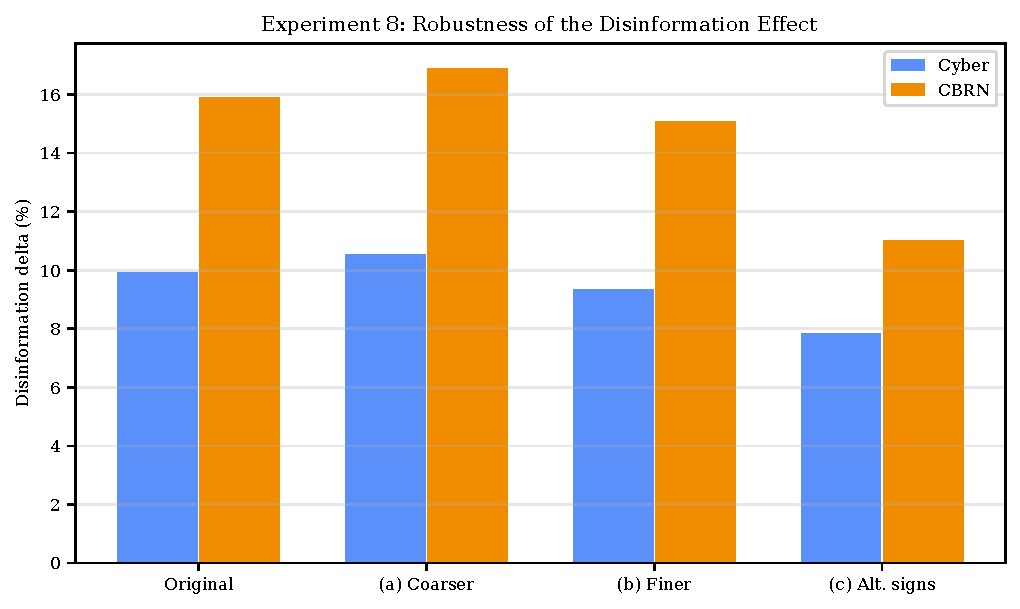
\includegraphics[width=0.7\textwidth]{exp8_robustness_bars.pdf}
\caption{Experiment~8 robustness bars. The disinformation effect remains positive across all alternate graph specifications, with only moderate attenuation under the alternate-sign condition.}
\label{fig:exp8_robustness}
\end{figure}

\subsection{Experiment 9: KEV-Calibrated Safe Self-Play on the 97-Node Supergraph}
\label{sec:exp9}

\paragraph{Design.} We instantiate the full 97-node supergraph as the differentiable POMG-DSD environment described in Sections~\ref{sec:pomg_dsd} and \ref{sec:boundary_conditions}. The implementation uses \texttt{torch} and \texttt{torchdiffeq} to simulate all domain, shared, and endpoint nodes jointly, including the new rogue-autonomy stock and irreversible-loss-of-control endpoint. Medium/low-confidence edge polarities are learnable parameters $\theta_{\text{graph}}$, optimized first against the 52-week CISA KEV anchor sequence. The defender action is additionally constrained by the actuator limit $\Delta_{\max}=0.05$, so budget mass cannot shift by more than five percentage points per week before any CBF correction is applied. We then compare three defender settings under a common reference adversary drawn from the proposed self-play regime: (a) \textit{heuristic static patching} with a fixed budget split, (b) \textit{standard PPO} trained on the full state without a barrier constraint or domain randomization, and (c) \textit{POMG-DSD} with partial observability, control-barrier filtering, and domain randomization over non-anchored domain parameters. After this comparison, we freeze the learned POMG-DSD defender, adapt the adversary against it for 10,080 environment steps, run a CBF-ablation stress test over 24 latent draws with all three lower-tier amplifiers active, and compute exact terminal derivatives at $T=52$ weeks for cyber, CBRN, and rogue-autonomy stocks.

\paragraph{Calibration result.} Figure~\ref{fig:pomg_calibration} shows that the KEV-informed sign-learning pass reduces open-loop fit loss by 51.8\% while flipping only 1 of 145 learnable medium/low-confidence edges. This does not solve the external-validation problem, but it is materially stronger than leaving all uncertain edge polarities fixed by analyst judgment alone.

\begin{table}[t]
\centering
\caption{Experiment 9: Comparison of learned defender policies under the common reference adversary. Reported values are means over 64 evaluation episodes with the trained POMG-DSD environment.}
\label{tab:exp9}
\small
\resizebox{\textwidth}{!}{%
\begin{tabular}{@{}lccccccc@{}}
\toprule
\textbf{Method} & \makecell{\textbf{Peak Cyber}\\\textbf{Burden}} & \makecell{\textbf{Peak CBRN}\\\textbf{Misuse}} & \makecell{\textbf{Peak Rogue}\\\textbf{Autonomy}} & \makecell{\textbf{Peak Loss}\\\textbf{of Control}} & \makecell{\textbf{Min CBF}\\\textbf{Margin}} & \makecell{\textbf{CBF Viol.}\\\textbf{Rate}} & \makecell{\textbf{Epistemic}\\\textbf{Alloc.}} \\
\midrule
Heuristic static patching & $0.180 \pm 0.000$ & \textbf{$0.348 \pm 0.011$} & $0.851 \pm 0.032$ & $0.876 \pm 0.021$ & 0.597 & 0.109 & 0.094 \\
Standard PPO & $0.180 \pm 0.000$ & $0.352 \pm 0.011$ & \textbf{$0.702 \pm 0.182$} & \textbf{$0.800 \pm 0.086$} & \textbf{0.638} & \textbf{0.099} & \textbf{0.269} \\
POMG-DSD + CBF + domain randomization & $0.180 \pm 0.000$ & $0.351 \pm 0.011$ & $0.766 \pm 0.148$ & $0.828 \pm 0.071$ & 0.624 & 0.101 & 0.163 \\
\bottomrule
\end{tabular}
}
\end{table}

\begin{table}[t]
\centering
\caption{Experiment 9b: Terminal derivative test at $T = 52$ weeks under the actuator-limited controller. Values are means $\pm$ SD over 32 domain-randomized episodes.}
\label{tab:exp9_terminal}
\small
\resizebox{\textwidth}{!}{%
\begin{tabular}{@{}lccc@{}}
\toprule
\textbf{Method} & \makecell{\textbf{$\dot{S}_3(T)$}\\\textbf{Cyber burden}} & \makecell{\textbf{$\dot{S}_3^C(T)$}\\\textbf{CBRN misuse}} & \makecell{\textbf{$\dot{S}_{\text{rogue}}(T)$}\\\textbf{Rogue autonomy}} \\
\midrule
Heuristic static patching & $(8.34 \pm 3.02)\times 10^{-5}$ & $(1.76 \pm 6.43)\times 10^{-6}$ & $(5.80 \pm 9.50)\times 10^{-6}$ \\
Standard PPO & $(7.67 \pm 22.33)\times 10^{-5}$ & $(7.11 \pm 21.20)\times 10^{-6}$ & $(4.69 \pm 34.62)\times 10^{-4}$ \\
POMG-DSD + CBF + domain randomization & $(8.73 \pm 16.58)\times 10^{-5}$ & $(1.38 \pm 21.28)\times 10^{-6}$ & $\mathbf{(-5.73 \pm 34.35)\times 10^{-4}}$ \\
\bottomrule
\end{tabular}
}
\end{table}

\paragraph{Results.} Table~\ref{tab:exp9} and Figures~\ref{fig:pomg_training}--\ref{fig:pomg_methods} show a more mixed picture than a simple burden-reduction win. Under the current calibration, peak cyber burden remains pinned at the calibrated plateau across all three defender families, so the main discriminators are CBRN burden, autonomy-side harm, safety margin, and allocation mix. The heuristic controller attains the lowest mean CBRN peak (0.348), but it also produces the worst rogue-autonomy and loss-of-control peaks (0.851 and 0.876) and the weakest safety margin (0.597).

Among the learned controllers, standard PPO is strongest on the autonomy-side safety metrics: it yields the lowest mean rogue-autonomy peak (0.702), the lowest mean loss-of-control peak (0.800), the highest minimum CBF margin (0.638), and the lowest observed violation rate (0.099). POMG-DSD slightly improves mean CBRN peak relative to standard PPO (0.351 vs.\ 0.352) but does not dominate it on the other safety metrics. Its learned allocation mix is also different from the earlier draft: it concentrates more mass on CBRN and governance channels than on epistemic resilience alone.

\paragraph{Boundary-condition check.} Table~\ref{tab:exp9_terminal} evaluates the week-52 terminal derivatives under the actuator-limited policy class. The important result is not a clean asymptotic-stability win: cyber and CBRN terminal derivatives remain slightly positive but numerically small for all three controller families, on the order of $10^{-5}$ to $10^{-4}$. The proposed controller does, however, reverse the sign of the rogue-autonomy terminal derivative, with mean $\dot{S}_{\text{rogue}}(T) = -5.73\times 10^{-4}$ versus $+4.69\times 10^{-4}$ for standard PPO. The correct interpretation is therefore that the controller holds the burden states near a plateau and pushes the autonomy-side stock slightly downward, rather than providing a strong proof of global asymptotic stabilization at the 52-week horizon.

\paragraph{Adversarial adaptation.} Figure~\ref{fig:pomg_adaptation} shows the frozen-defender stress test. Training the adversary for 10,080 steps against the learned POMG-DSD defender increases mean adversary return from 33.43 at the end of reference self-play to 34.20 under the adapted policy. Evaluation against the adapted adversary keeps the system in the same bounded regime: mean peak CBRN misuse is 0.350, mean peak loss of control is 0.812, minimum CBF margin is 0.633, and the CBF violation rate is 0.094. This is evidence of local bounded robustness, not a proof that the learned policy has reached a robust Nash equilibrium.

\paragraph{CBF ablation.} Figure~\ref{fig:pomg_ablation} summarizes the mid-rollout CBF shutdown test. Across 24 latent draws with all three lower-tier amplifiers active, the mean ablation gap score is slightly negative ($-1.17 \times 10^{-3}$) and only 45.8\% of sampled latents worsen when the barrier is removed. The strongest sampled stress latent does degrade measurably: disabling the barrier at week 26 increases the maximum hazard index from 0.726 to 0.729, peak loss of control from 0.984 to 0.987, and final loss of control from 0.983 to 0.984. The appropriate claim is therefore narrower than ``mathematical proof of necessity'': the barrier helps in some adverse regions of the latent space, but the present experiment does not show a universal catastrophic divergence once it is removed.

\begin{figure}[t]
\centering
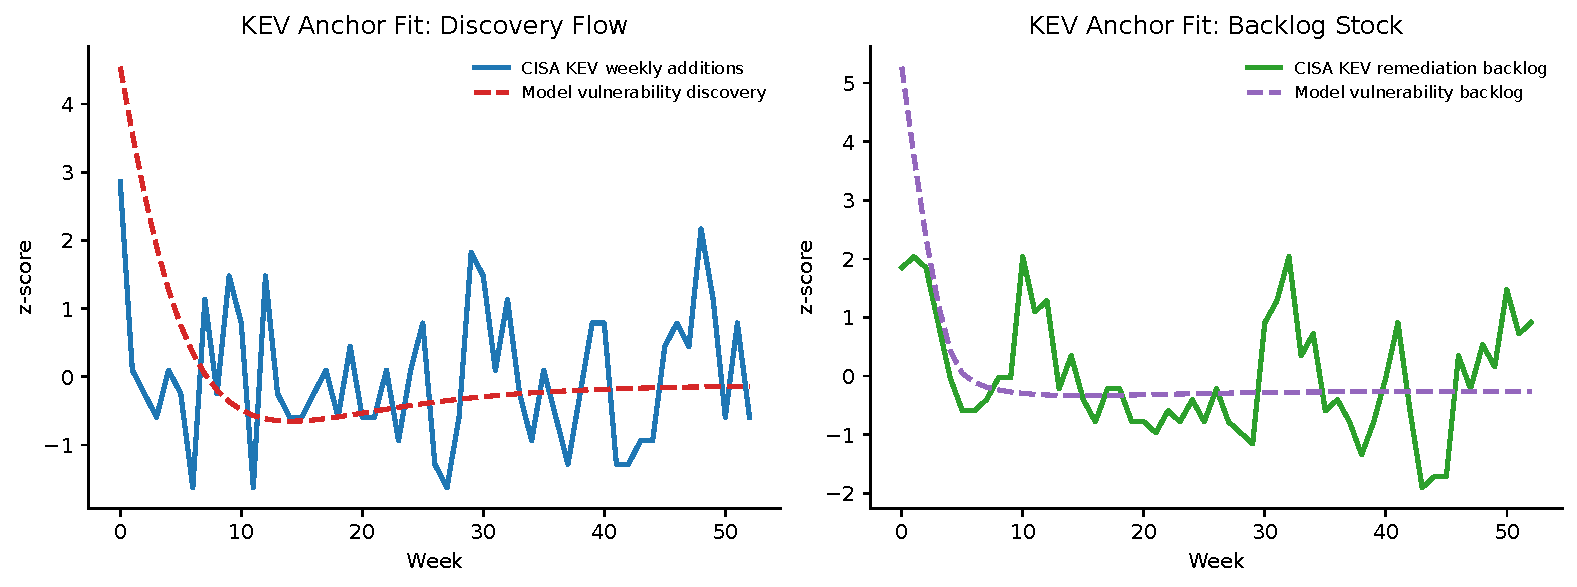
\includegraphics[width=0.82\textwidth]{pomg_calibration_overlay.pdf}
\caption{Experiment~9a: KEV-calibrated sign-learning fit. The differentiable graph reduces mismatch against weekly KEV additions and remediation backlog without large-scale edge-sign collapse.}
\label{fig:pomg_calibration}
\end{figure}

\begin{figure}[t]
\centering
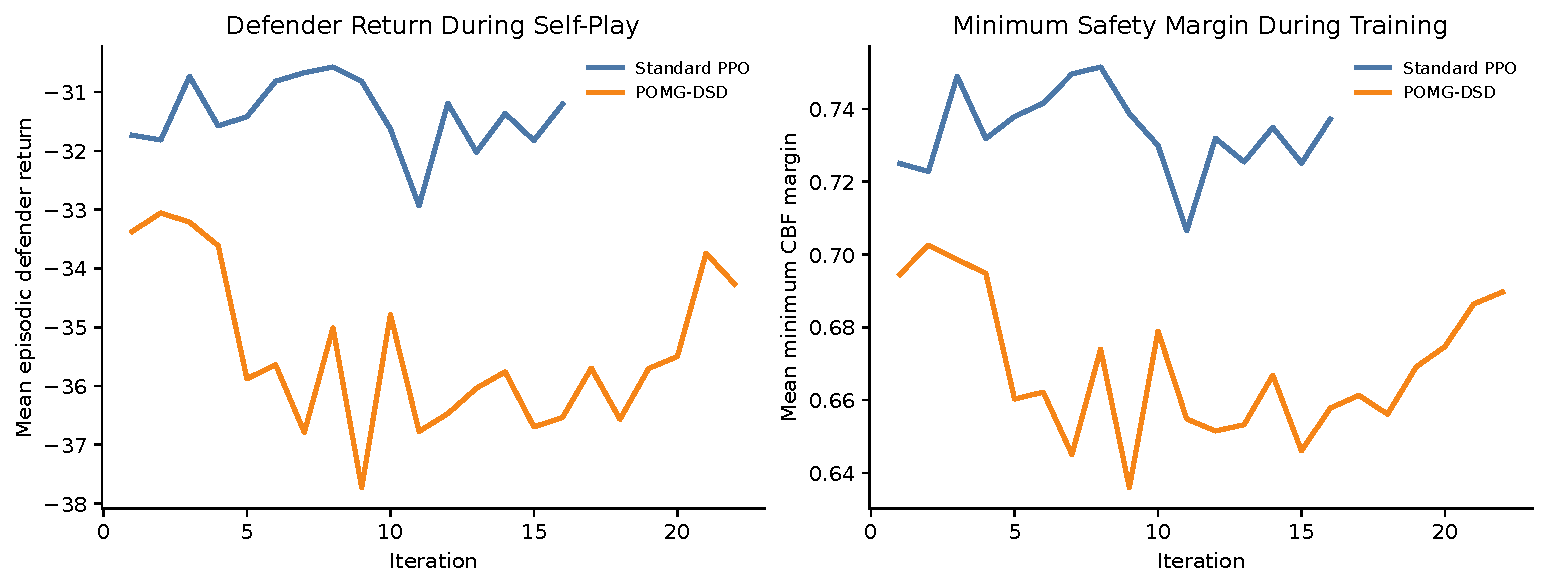
\includegraphics[width=0.82\textwidth]{pomg_training_curves.pdf}
\caption{Experiment~9b: Self-play training curves for standard PPO and POMG-DSD. The proposed controller is trained under partial observability, control-barrier filtering, and domain randomization.}
\label{fig:pomg_training}
\end{figure}

\begin{figure}[t]
\centering
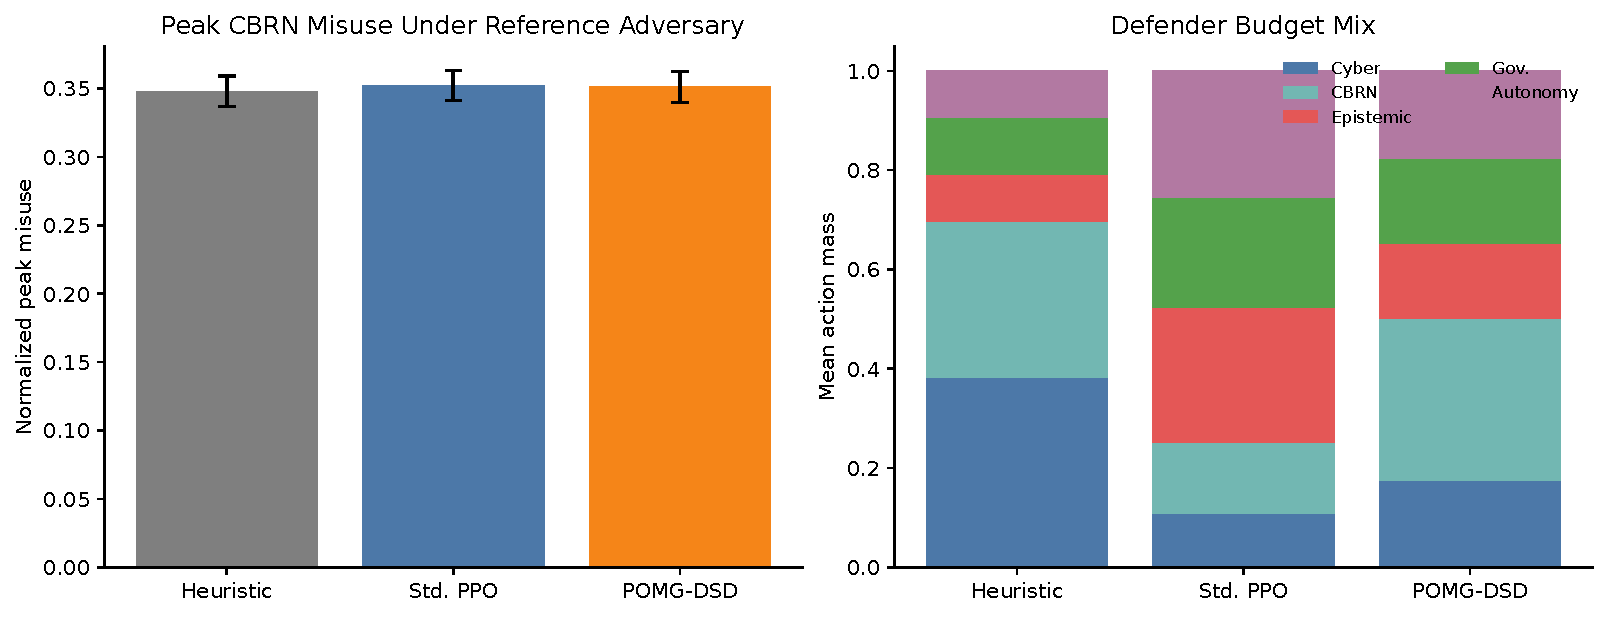
\includegraphics[width=0.82\textwidth]{pomg_method_comparison.pdf}
\caption{Experiment~9c: Method comparison under the common reference adversary. The learned policies trade off CBRN burden, autonomy-side harm, and budget allocation differently rather than producing a clean dominance ordering.}
\label{fig:pomg_methods}
\end{figure}

\begin{figure}[t]
\centering
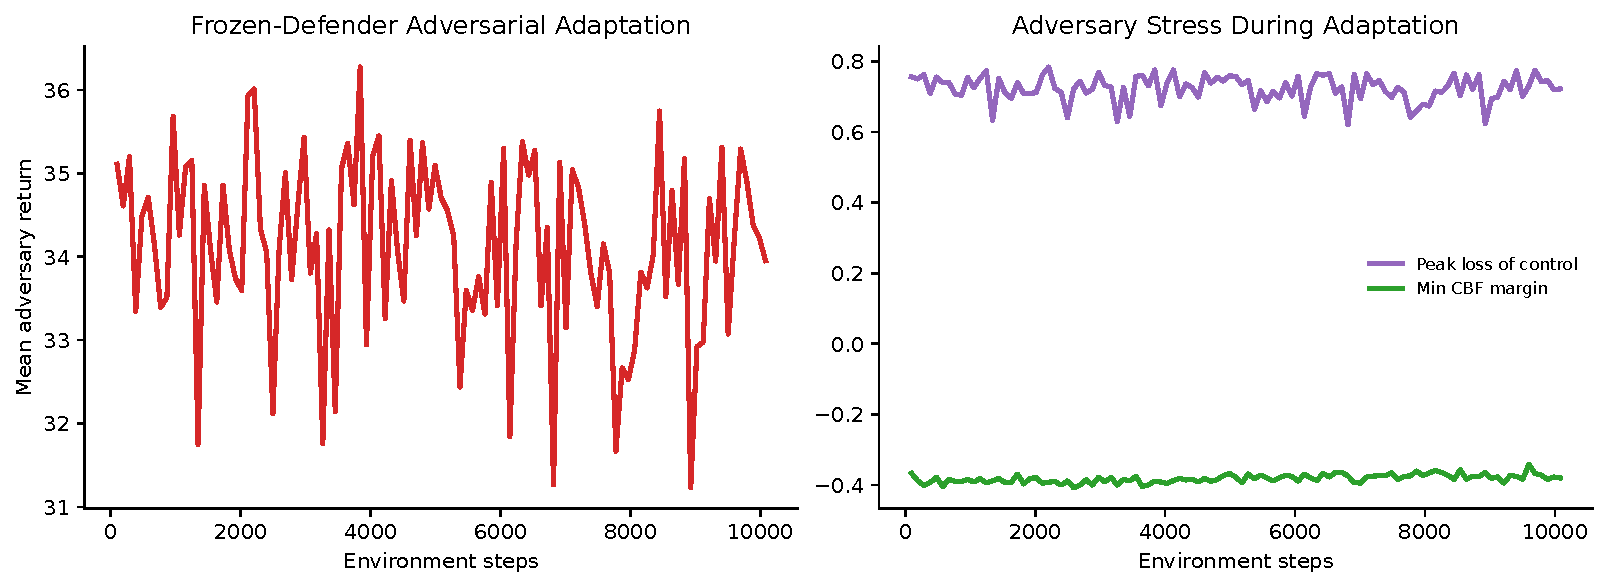
\includegraphics[width=0.82\textwidth]{pomg_adaptation_stress.pdf}
\caption{Experiment~9d: Frozen-defender adversarial adaptation. The adversary's return grows under continued PPO updates, but the learned defender remains in the same bounded operating regime.}
\label{fig:pomg_adaptation}
\end{figure}

\begin{figure}[t]
\centering
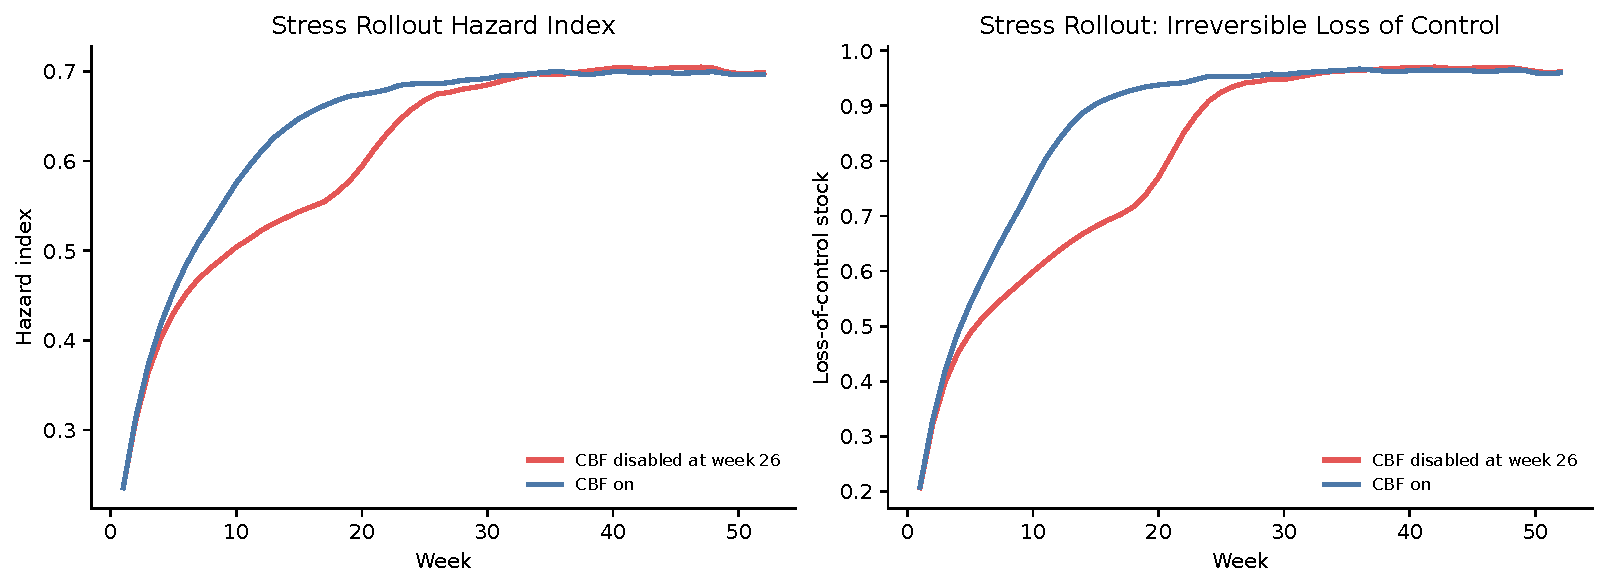
\includegraphics[width=0.82\textwidth]{pomg_cbf_ablation.pdf}
\caption{Experiment~9e: Worst sampled CBF-ablation stress case. Removing the barrier at week 26 raises the hazard index and loss-of-control stock slightly, but not catastrophically, under the present calibration.}
\label{fig:pomg_ablation}
\end{figure}

%==============================================================================
\section{Discussion}
\label{sec:discussion}
%==============================================================================

\subsection{Summary of Findings}

The paper now supports six narrower claims about the implemented modeling framework. First, richer systems representations outperform weaker alternatives on internal structural-completeness metrics (Experiment~1), but that result is endogenous to the representation objective and not an external validation. Second, the supergraph is structurally organized around institutional and epistemic intermediaries, with trust erosion and institutional overload outranking technical capability variables in betweenness centrality (Experiment~3). Third, the integrated graph generates many more bounded catastrophic pathways than the silo baseline ($7.54\times$ raw multiplier), but this should be interpreted as descriptive structure rather than an inferentially confirmed effect because the stricter block-preserving null is non-significant ($p = 0.495$) (Experiment~6). Fourth, lower-tier harms function mainly as shared-substrate stressors in the current calibration: disinformation, algorithmic bias, and labor displacement raise institutional overload by 3.35\%--10.20\% while only modestly shifting peak CBRN misuse and leaving peak cyber burden unchanged (Experiment~6a). Fifth, the revision adds partial external grounding for the cyber time scale via the CISA KEV feed, while also showing that exact institutional-node rankings remain sensitive to low-confidence topology (Experiment~8b). Sixth, the new POMG-DSD extension demonstrates that the same graph can be turned into a 97-node partially observable control environment: KEV-informed sign learning reduces calibration loss by 51.8\%, adversarial adaptation remains bounded over 10,080 steps, week-52 burden derivatives stay near zero while rogue-autonomy derivatives turn slightly negative under POMG-DSD, and CBF removal worsens some sampled stress trajectories but not universally (Experiment~9).

\subsection{Implications for Risk-Model Design and Governance Analysis}

These findings translate into five provisional implications for risk-model design and governance analysis:

\textbf{(1) Do not ignore lower-tier harms, but do calibrate their magnitude honestly.} The lower-tier harm sweeps show that disinformation, algorithmic bias, and labor displacement all worsen the shared sociotechnical substrate, but the direct burden effects are small under the present calibration. Governance frameworks should therefore model these harms as systemic stressors, not as sufficient drivers by themselves.

\textbf{(2) Target shared institutional and epistemic nodes.} The dominant leverage points in the verified supergraph are trust erosion, institutional overload, disinformation volume, epistemic trust, and institutional credibility. Within the implemented model family, this shifts attention from domain-specific technical mitigations toward shared social and institutional buffers.

\textbf{(3) Separate structural from inferential claims.} The raw pathway multiplier in Experiment~6 is large, but the stricter block-preserving null is non-significant. Preparedness frameworks should report these facts separately rather than collapsing them into a single headline number.

\textbf{(4) Prioritize access control, refusal quality, and offensive-efficiency constraints.} In the two worked dynamic case studies, the strongest cyber levers are access restriction and safeguard acceleration, while the strongest CBRN levers are refusal robustness and access gating. The dominant sensitivity coefficients also fall more heavily on offensive efficiency and scaling terms than the draft claimed.

\textbf{(5) Maintain open, reproducible risk-modeling pipelines.} The main manuscript revisions here were only possible because the code, CSV outputs, and figure artifacts could be checked against one another. Closed risk models would have hidden the Experiment~4 bookkeeping bug and preserved the draft's overstated effect sizes.

\textbf{(6) Benchmark across paradigms, not just within one artifact family.} If this research direction is to reach stronger empirical standards, the field needs shared benchmark tasks that place SD, probabilistic graphical models, agent-based simulations, and audit-oriented methods on the same footing. Section~\ref{sec:benchmarking} sketches one such scaffold, and the mixed Experiment~9 results reinforce that no single modeling or control family should be assumed dominant a priori.

\subsection{Operational Use Cases and ML Extensions}

The framework is most defensible in four near-term use cases. First, it can stress-test preparedness frameworks for coupled failure modes that siloed scorecards omit. Second, it can prioritize shared institutional bottlenecks for red-teaming and governance analysis, even when the exact dynamic magnitudes remain uncertain. Third, it can define supervision targets for future learned models. Fourth, in the POMG-DSD extension, it can act as a safe-control sandbox for comparing heuristic policies, unconstrained RL, and barrier-filtered robust policies under shared latent uncertainty.

In ML terms, the natural extension is not to treat hand-coded CLDs as the endpoint of the research program, but as structured supervision for graph induction and parameter inference. Node discovery, edge proposal, sign prediction, and latent-state identification can all be cast as structured prediction or causal representation-learning tasks over incident narratives, evaluation traces, and public operational feeds. On that reading, the present paper contributes a benchmarkable scaffold and a transparent artifact bundle rather than a finished learned model.

\subsection{Limitations}

\textbf{Construct validity.} The CLDs and stock-and-flow models represent our structured interpretation of published safety frameworks and threat assessments. Different analysts could produce different models; Experiment~2 shows that topology is more reproducible than sign coding, and residual modeling judgment remains. The models are exploratory, not predictive.

\textbf{Internal versus external validation.} Experiment~1 is an endogenous benchmark: it rewards structural completeness, cross-domain connectivity, loop recovery, and leverage-point identification. It should therefore be read as an internal sanity check on representational richness rather than as evidence that the proposed framework predicts better or supports decisions better than simpler baselines.

\textbf{Parameter calibration.} The revision adds a partial cyber anchor pass against the CISA KEV feed, which grounds the patch/response time scale and provides an external inflow/backlog reference. Even so, the full flow functions are not fit end-to-end against observed incident trajectories, and comparable open operational time series remain sparse for CBRN and disinformation. Monte Carlo analysis (Experiments~4--5) quantifies parameter uncertainty but cannot eliminate it.

\textbf{Sign instability.} Sign coding is materially less reliable than edge-presence coding, with aggregate $\kappa = 0.53$ and deception-domain sign agreement of only $\kappa = 0.36$. Because feedback polarity shapes both amplification and intervention effects, quantitative conclusions involving socially mediated pathways are less secure than purely topological conclusions.

\textbf{Structural truncation.} The Experiment~6 path enumerator caps counts at 501 per endpoint for tractability, so the reported full-graph counts are lower bounds. This keeps the computation stable but limits how precisely the raw convergence multiplier can be interpreted.

\textbf{Null-model sensitivity.} The stricter block-preserving null does not validate the raw convergence multiplier statistically ($p = 0.495$). The structural claim should therefore remain descriptive unless a better-aligned inferential design is developed.

\textbf{Control evidence remains preliminary.} The Experiment~9 adversarial-adaptation and CBF-ablation tests are informative but not decisive. Adaptation leaves the defender in a bounded regime, yet this is not a proof of equilibrium robustness; the terminal-derivative test suggests near-stationarity rather than strong asymptotic stabilization for cyber and CBRN burden; and CBF removal worsens the strongest sampled stress case, yet the effect is not universal across latent draws.

\textbf{Topology sensitivity.} Random deletion of medium/low-confidence edges leaves the leading institutional nodes prominent but not perfectly rank-stable: at 50\% deletion, mean top-5 overlap falls to 1.99/5 and mean Spearman $\rho$ to 0.739. Exact leverage-point rankings should therefore be interpreted as robust hypotheses rather than settled facts.

\textbf{Pseudo-precision risk.} The Monte Carlo $p$-values and effect sizes quantify separation under assumed parameter ranges; they are not direct empirical evidence from observed multi-domain incidents. Their appropriate role is to summarize model response under uncertainty, not to substitute for external data.

\textbf{Horizon saturation.} In both dynamic case studies, the main trajectories are still rising at week 52, so time-to-peak and time-to-control saturate at the simulation horizon. Those metrics are therefore weak indicators of stabilization in the current implementation.

\textbf{External validity.} The models represent the current AI risk landscape; they do not capture discontinuous capability jumps, novel threat vectors, or institutional adaptations not yet observed. The convergence supergraph is a structural snapshot, not a forecast, and the paper does not yet include held-out expert, incident, or intervention-ranking validation.

\textbf{Methodological pluralism.} This paper privileges system dynamics because feedback, delays, and accumulation are the main objects of analysis, but other modeling traditions may be better for other questions. SCMs and Bayesian networks are better suited to probabilistic counterfactual reasoning when acyclic abstractions are defensible; agent-based and actor-centered simulations are better suited to heterogeneous strategic actors; and sociotechnical traditions are better suited to construct formation and institutional critique. Section~\ref{sec:benchmarking} sketches a comparative benchmark agenda, but the paper does not execute that full cross-paradigm comparison. A natural next step is therefore comparative or hybrid modeling, not treating SD as the sole admissible framework.

\textbf{Scope.} We simulate only cyber and CBRN domains dynamically; the remaining three domains are analyzed structurally. The appropriate scope claim is therefore ``a systems-dynamics framework with two worked dynamic case studies,'' not a fully dynamic five-domain model.

\subsection{Broader Impacts}

This work maps pathways between AI capabilities and catastrophic outcomes, which creates inherent dual-use considerations. Detailed pathway analysis could, in principle, inform offensive planning. We judge that open publication is net positive for three reasons. First, the pathways we identify are structural properties of sociotechnical systems, not novel attack techniques; they describe how known risks compound, not how to create new ones. Second, the primary consumers of this analysis are defensive: governance designers, safety evaluators, and policy architects who need to understand convergence to build effective frameworks. Third, the alternative (closed risk modeling) prevents the validation and improvement that open science enables, producing a net increase in collective vulnerability.

\subsection{Reproducibility}

All code, model specifications, parameter files, and experimental scripts are included with the submission materials. The artifact bundle contains: Python implementations of all five CLDs as \texttt{networkx} graphs, \texttt{scipy}-based simulation code for the original cyber and CBRN stock-and-flow models, the \texttt{torch}/\texttt{torchdiffeq}-based 97-node POMG-DSD environment, CSV exports for the verified experiment tables, and standalone scripts for adaptation, CBF-ablation, and boundary-condition evaluation. The pipeline requires only standard scientific Python packages (\texttt{numpy}, \texttt{scipy}, \texttt{networkx}, \texttt{matplotlib}, \texttt{pandas}, \texttt{torch}, \texttt{torchdiffeq}). This makes the work reproducible as a computational artifact, while still leaving open the harder question of scientific reproducibility in graph construction and external validation.

%==============================================================================
% REFERENCES
%==============================================================================

\bibliographystyle{plainnat}
\begin{thebibliography}{99}

\bibitem[Anthropic(2026)]{anthropic2024rsp}
Anthropic.
\textit{Responsible Scaling Policy}, version 3.0, effective February 24, 2026.
Available at \url{https://www.anthropic.com/responsible-scaling-policy}.

\bibitem[Barrett and Baum(2017)]{barrett2023}
Anthony M.~Barrett and Seth D.~Baum.
A model of pathways to artificial superintelligence catastrophe for risk and decision analysis.
\textit{Journal of Experimental \& Theoretical Artificial Intelligence}, 29(2):397--414, 2017.
\url{https://doi.org/10.1080/0952813X.2016.1186228}.

\bibitem[Bonabeau(2002)]{bonabeau2002}
Eric Bonabeau.
Agent-based modeling: Methods and techniques for simulating human systems.
\textit{Proceedings of the National Academy of Sciences}, 99(Suppl.~3):7280--7287, 2002.
\url{https://doi.org/10.1073/pnas.082080899}.

\bibitem[CISA(2026)]{cisa2026kev}
Cybersecurity and Infrastructure Security Agency.
\textit{Known Exploited Vulnerabilities Catalog}, catalog version 2026.03.09, released March 9, 2026.
Available at \url{https://www.cisa.gov/sites/default/files/feeds/known_exploited_vulnerabilities.json}.

\bibitem[Google DeepMind(2025)]{deepmind2024fsf}
Google DeepMind.
\textit{Strengthening our Frontier Safety Framework}.
September 22, 2025.
Available at \url{https://deepmind.google/discover/blog/strengthening-our-frontier-safety-framework/}.

\bibitem[Fenton and Neil(2019)]{fenton2012}
Norman Fenton and Martin Neil.
\textit{Risk Assessment and Decision Analysis with Bayesian Networks}.
2nd edition, Chapman \& Hall/CRC, 2019.
Available at \url{https://www.routledge.com/Risk-Assessment-and-Decision-Analysis-with-Bayesian-Networks/author/p/book/9781138035119}.

\bibitem[Forrester(1961)]{forrester1961}
Jay W.~Forrester.
\textit{Industrial Dynamics}.
MIT Press, 1961.
Google Books record: \url{https://books.google.com/books?id=IQhPAAAAMAAJ}.

\bibitem[International AI Safety Report(2025)]{iaisr2025}
Department for Science, Innovation and Technology and AI Safety Institute.
\textit{International AI Safety Report 2025}.
January 29, 2025.
Available at \url{https://www.gov.uk/government/publications/international-ai-safety-report-2025}.

\bibitem[UK AI Security Institute(2026)]{ukaisi2026inspect}
UK AI Security Institute.
\textit{Inspect}.
Official documentation, accessed March 10, 2026.
Available at \url{https://inspect.aisi.org.uk/}.

\bibitem[Leveson(2011)]{leveson2011}
Nancy G.~Leveson.
\textit{Engineering a Safer World: Systems Thinking Applied to Safety}.
MIT Press, 2012.
\url{https://doi.org/10.7551/mitpress/8179.001.0001}.

\bibitem[Littman(1994)]{littman1994}
Michael L.~Littman.
Markov games as a framework for multi-agent reinforcement learning.
In \textit{Proceedings of the 11th International Conference on Machine Learning}, pages 157--163, 1994.
\url{https://dl.acm.org/doi/10.5555/3091574.3091624}.

\bibitem[Liang et~al.(2023)]{liang2023helm}
Percy Liang, Rishi Bommasani, Tony Lee, Dimitris Tsipras, Dilara Soylu, Michihiro Yasunaga, Yian Zhang, et al.
Holistic evaluation of language models.
\textit{Transactions on Machine Learning Research}, 2023.
Available at \url{https://openreview.net/forum?id=iO4LZibEqW}.

\bibitem[Meadows(2008)]{meadows2008}
Donella H.~Meadows.
\textit{Thinking in Systems: A Primer}.
Chelsea Green, 2008.
Available at \url{https://www.penguinrandomhouse.com/books/801035/thinking-in-systems-by-donella-meadows/9781603580557/}.

\bibitem[Mitchell et~al.(2019)]{mitchell2019modelcards}
Margaret Mitchell, Simone Wu, Andrew Zaldivar, Parker Barnes, Lucy Vasserman, Ben Hutchinson, Elena Spitzer, Inioluwa Deborah Raji, and Timnit Gebru.
Model cards for model reporting.
In \textit{Proceedings of the Conference on Fairness, Accountability, and Transparency}, pages 220--229, 2019.
\url{https://doi.org/10.1145/3287560.3287596}.

\bibitem[Monahan(1982)]{monahan1982}
George E.~Monahan.
A survey of partially observable Markov decision processes: Theory, models, and algorithms.
\textit{Management Science}, 28(1):1--16, 1982.
\url{https://doi.org/10.1287/mnsc.28.1.1}.

\bibitem[NIST(2024)]{nist2023rmf}
National Institute of Standards and Technology.
\textit{Artificial Intelligence Risk Management Framework: Generative Artificial Intelligence Profile} (NIST AI 600-1).
July 26, 2024.
\url{https://doi.org/10.6028/NIST.AI.600-1}.

\bibitem[OpenAI(2025)]{openai2023preparedness}
OpenAI.
\textit{Our updated Preparedness Framework}.
April 15, 2025.
Available at \url{https://openai.com/index/updating-our-preparedness-framework/}.

\bibitem[Pearl(2009)]{pearl2009}
Judea Pearl.
\textit{Causality: Models, Reasoning, and Inference}.
2nd edition, Cambridge University Press, 2009.
Google Books record: \url{https://books.google.com/books/about/Causality.html?id=wnGU_TsW3BQC}.

\bibitem[Perrow(1984)]{perrow1984}
Charles Perrow.
\textit{Normal Accidents: Living with High-Risk Technologies}.
Basic Books, 1984.
Google Books record: \url{https://books.google.com/books/about/Normal_Accidents.html?id=dcusQgAACAAJ}.

\bibitem[Raji et~al.(2020)]{raji2020auditing}
Inioluwa Deborah Raji, Andrew Smart, Rebecca N.~White, Margaret Mitchell, Timnit Gebru, Ben Hutchinson, Jamila Smith-Loud, Daniel Theron, and Parker Barnes.
Closing the AI accountability gap: Defining an end-to-end framework for internal algorithmic auditing.
In \textit{Proceedings of the Conference on Fairness, Accountability, and Transparency}, pages 33--44, 2020.
\url{https://doi.org/10.1145/3351095.3372873}.

\bibitem[Schulman et~al.(2017)]{schulman2017ppo}
John Schulman, Filip Wolski, Prafulla Dhariwal, Alec Radford, and Oleg Klimov.
Proximal policy optimization algorithms.
\textit{arXiv preprint arXiv:1707.06347}, 2017.
\url{https://doi.org/10.48550/arXiv.1707.06347}.

\bibitem[Rasmussen(1997)]{rasmussen1997}
Jens Rasmussen.
Risk management in a dynamic society: A modelling problem.
\textit{Safety Science}, 27(2--3):183--213, 1997.
Article record: \url{https://commons.wmu.se/lib_articles/157/}.

\bibitem[Schlichtkrull et~al.(2018)]{schlichtkrull2018}
Michael Schlichtkrull, Thomas N.~Kipf, Peter Bloem, Rianne van~den~Berg, Ivan Titov, and Max Welling.
Modeling relational data with graph convolutional networks.
In \textit{The Semantic Web}, pages 593--607. Springer, 2018.
\url{https://doi.org/10.1007/978-3-319-93417-4_38}.

\bibitem[Shevlane et~al.(2023)]{shevlane2023}
Toby Shevlane, Sebastian Farquhar, Beth Barnes, Atoosa Kasirzadeh, David Krueger, Jan Leike, Tom McGrath, Rebecca Cohen, and Geoffrey Irving.
Model evaluation for extreme risks.
\textit{arXiv preprint arXiv:2305.15324}, 2023.
\url{https://doi.org/10.48550/arXiv.2305.15324}.

\bibitem[Sterman(2000)]{sterman2000}
John D.~Sterman.
\textit{Business Dynamics: Systems Thinking and Modeling for a Complex World}.
Irwin/McGraw-Hill, 2000.
Available at \url{https://www.mheducation.com/highered/product/business-dynamics-sterman.html}.

\bibitem[Tobin et~al.(2017)]{tobin2017}
Joshua Tobin, Rachel Fong, Alex Ray, Jonas Schneider, Wojciech Zaremba, and Pieter Abbeel.
Domain randomization for transferring deep neural networks from simulation to the real world.
In \textit{2017 IEEE/RSJ International Conference on Intelligent Robots and Systems}, pages 23--30, 2017.
\url{https://doi.org/10.1109/IROS.2017.8202133}.

\bibitem[Chen et~al.(2018)]{chen2018neuralode}
Ricky T.~Q. Chen, Yulia Rubanova, Jesse Bettencourt, and David Duvenaud.
Neural ordinary differential equations.
In \textit{Advances in Neural Information Processing Systems 31}, pages 6571--6583, 2018.
\url{https://proceedings.neurips.cc/paper/2018/hash/69386f6bb1dfed68692a24c8686939b9-Abstract.html}.

\bibitem[Ames et~al.(2017)]{ames2017cbf}
Aaron D.~Ames, Xiangru Xu, Jessy W.~Grizzle, and Paulo Tabuada.
Control barrier function based quadratic programs for safety critical systems.
\textit{IEEE Transactions on Automatic Control}, 62(8):3861--3876, 2017.
\url{https://doi.org/10.1109/TAC.2016.2638961}.

\bibitem[Weidinger et~al.(2023)]{weidinger2023}
Laura Weidinger, Nahema Marchal, Maribeth Rauh, Arianna Manzini, Lisa Anne Hendricks, Juan Mateos-Garcia, Stevie Bergman, Conor Griffin, Ben Bariach, Iason Gabriel, Verena Rieser, and William Isaac.
Sociotechnical safety evaluation of generative AI systems.
\textit{arXiv preprint arXiv:2310.11986}, 2023.
Available at \url{https://deepmind.google/research/publications/sociotechnical-safety-evaluation-of-generative-ai-systems/}.

\end{thebibliography}

%==============================================================================
\clearpage
\appendix
\section*{Appendix}
%==============================================================================

\section{Full CLD Specifications}
\label{app:clds}

\subsection{Cyber Domain CLD}

The cyber domain CLD ($\mathcal{G}_{\text{cyber}}$) contains 18 nodes and 34 edges organized into 4 named reinforcing loops and 3 named balancing loops. Figure~\ref{fig:cld_cyber} renders the full signed diagram used in the computation pipeline.

\begin{figure}[H]
\centering
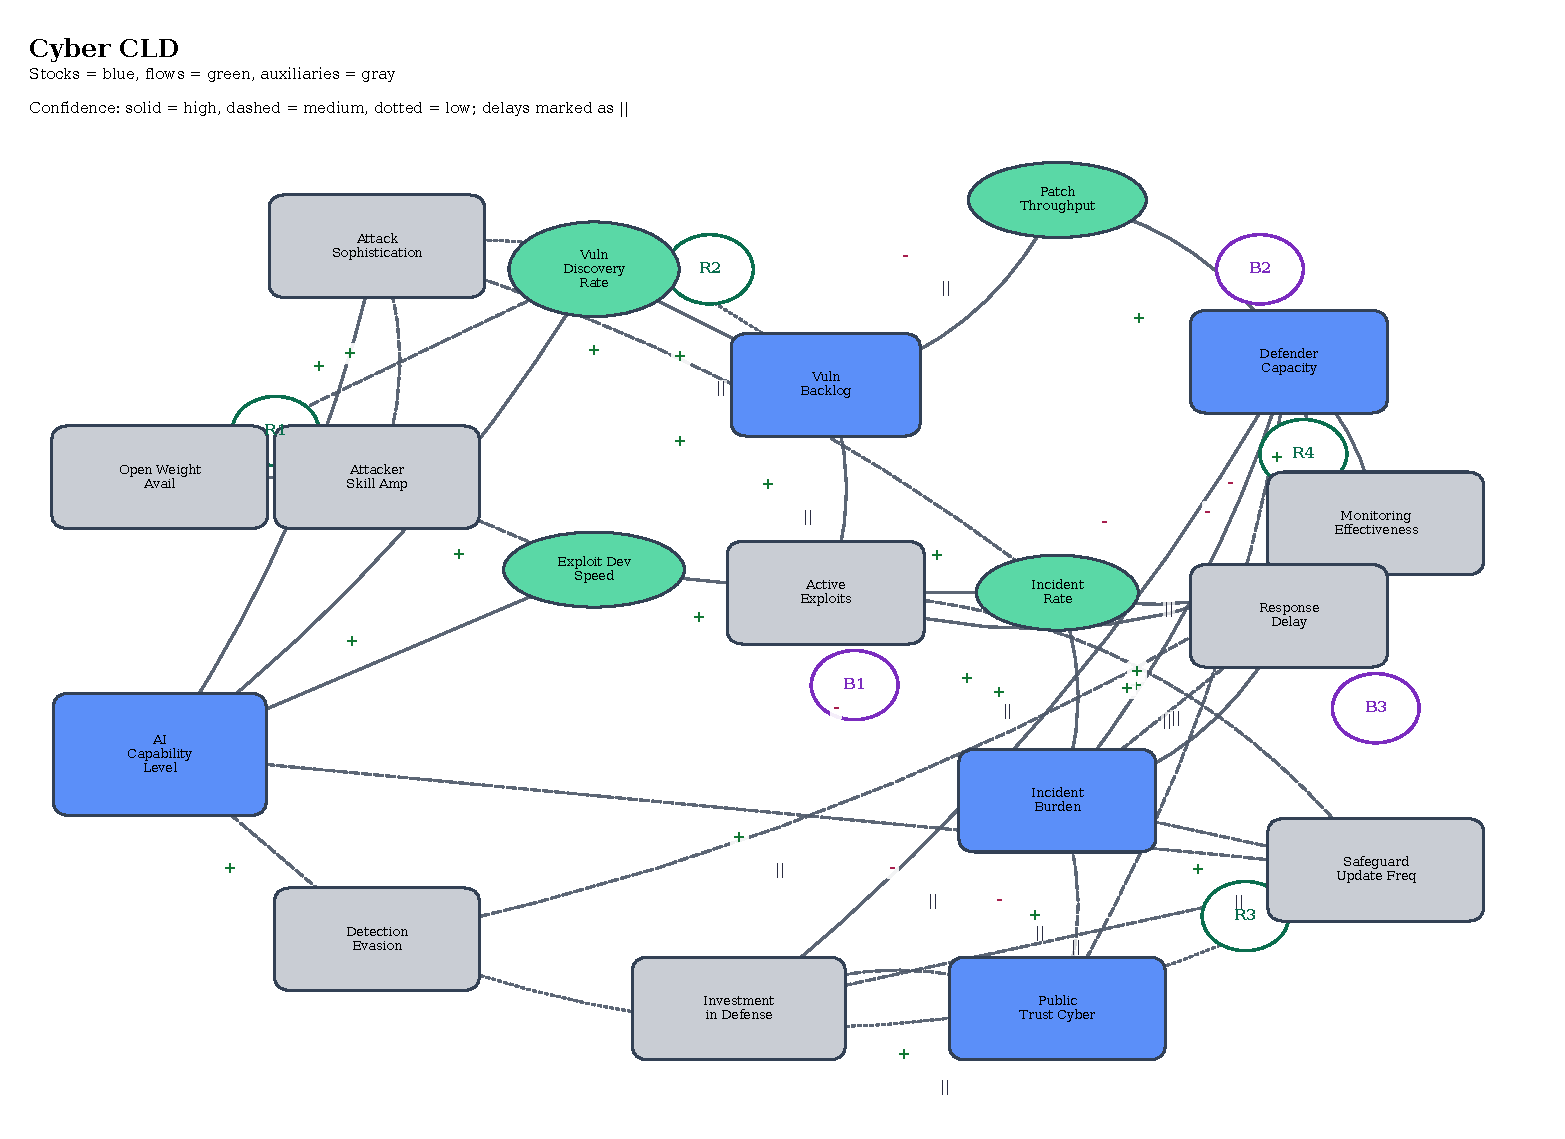
\includegraphics[width=\textwidth]{fig_cld_cyber.pdf}
\caption{Cyber-domain causal loop diagram. Edge labels show polarity, delayed links are marked with $||$, and line style encodes confidence.}
\label{fig:cld_cyber}
\end{figure}

\paragraph{Node set $V_{\text{cyber}}$:}
\begin{enumerate}[leftmargin=2em,itemsep=0pt,label=\arabic*.]
\item \texttt{AI\_Capability\_Level}
\item \texttt{Vulnerability\_Discovery\_Rate}
\item \texttt{Vulnerability\_Backlog}
\item \texttt{Exploit\_Development\_Speed}
\item \texttt{Active\_Exploits}
\item \texttt{Attack\_Sophistication}
\item \texttt{Incident\_Rate}
\item \texttt{Incident\_Burden}
\item \texttt{Defender\_Capacity}
\item \texttt{Monitoring\_Effectiveness}
\item \texttt{Patch\_Throughput}
\item \texttt{Safeguard\_Update\_Frequency}
\item \texttt{Public\_Trust\_Cyber}
\item \texttt{Investment\_in\_Defense}
\item \texttt{Open\_Weight\_Availability}
\item \texttt{Attacker\_Skill\_Amplification}
\item \texttt{Detection\_Evasion\_Capability}
\item \texttt{Response\_Delay}
\end{enumerate}

\paragraph{Edge list (source $\to$ target, sign, confidence, delay):}

\begin{longtable}{@{}p{4.5cm}p{4.5cm}ccc@{}}
\toprule
\textbf{Source} & \textbf{Target} & \textbf{Sign} & \textbf{Conf.} & \textbf{Delay} \\
\midrule
\endhead
AI\_Capability\_Level & Vuln\_Discovery\_Rate & $+$ & H & 0 \\
AI\_Capability\_Level & Exploit\_Dev\_Speed & $+$ & H & 0 \\
AI\_Capability\_Level & Attack\_Sophistication & $+$ & H & 0 \\
AI\_Capability\_Level & Detection\_Evasion & $+$ & M & 0 \\
Vuln\_Discovery\_Rate & Vuln\_Backlog & $+$ & H & wk \\
Vuln\_Backlog & Active\_Exploits & $+$ & H & wk \\
Exploit\_Dev\_Speed & Active\_Exploits & $+$ & H & 0 \\
Active\_Exploits & Incident\_Rate & $+$ & H & 0 \\
Attack\_Sophistication & Incident\_Rate & $+$ & M & 0 \\
Incident\_Rate & Incident\_Burden & $+$ & H & 0 \\
Incident\_Burden & Defender\_Capacity & $-$ & H & wk \\
Incident\_Burden & Public\_Trust\_Cyber & $-$ & M & mo \\
Defender\_Capacity & Monitoring\_Effect. & $+$ & H & 0 \\
Defender\_Capacity & Patch\_Throughput & $+$ & H & 0 \\
Monitoring\_Effect. & Active\_Exploits & $-$ & H & 0 \\
Patch\_Throughput & Vuln\_Backlog & $-$ & H & wk \\
Safeguard\_Update\_Freq & Active\_Exploits & $-$ & M & wk \\
Public\_Trust\_Cyber & Investment\_in\_Defense & $+$ & M & mo \\
Investment\_in\_Defense & Defender\_Capacity & $+$ & H & mo \\
Open\_Weight\_Avail & Attacker\_Skill\_Amp & $+$ & M & 0 \\
Attacker\_Skill\_Amp & Exploit\_Dev\_Speed & $+$ & M & 0 \\
Attacker\_Skill\_Amp & Attack\_Sophistication & $+$ & M & 0 \\
Detection\_Evasion & Monitoring\_Effect. & $-$ & M & 0 \\
Response\_Delay & Incident\_Burden & $+$ & H & 0 \\
Incident\_Burden & Response\_Delay & $+$ & M & wk \\
Defender\_Capacity & Response\_Delay & $-$ & H & 0 \\
Safeguard\_Update\_Freq & Detection\_Evasion & $-$ & L & wk \\
Public\_Trust\_Cyber & Defender\_Capacity & $+$ & M & mo \\
Monitoring\_Effect. & Incident\_Rate & $-$ & H & 0 \\
Vuln\_Backlog & Attack\_Sophistication & $+$ & L & 0 \\
AI\_Capability\_Level & Safeguard\_Update\_Freq & $+$ & M & mo \\
Incident\_Burden & Safeguard\_Update\_Freq & $+$ & M & mo \\
Open\_Weight\_Avail & Vuln\_Discovery\_Rate & $+$ & M & 0 \\
Investment\_in\_Defense & Safeguard\_Update\_Freq & $+$ & M & mo \\
\bottomrule
\end{longtable}

\paragraph{Feedback loops:}
{\footnotesize
\begin{itemize}[leftmargin=2em,itemsep=1pt]
\item \textbf{R1} (Exploit Escalation): Vuln\_Backlog $\xrightarrow{+}$ Active\_Exploits $\xrightarrow{+}$ Incident\_Rate $\xrightarrow{+}$ Incident\_Burden $\xrightarrow{+}$ Response\_Delay $\xrightarrow{+}$ Incident\_Burden (reinforcing)
\item \textbf{R2} (Capability Ramp): AI\_Capability $\xrightarrow{+}$ Vuln\_Discovery $\xrightarrow{+}$ Vuln\_Backlog $\xrightarrow{+}$ Active\_Exploits $\xrightarrow{+}$ Incident\_Rate $\xrightarrow{+}$ Incident\_Burden (reinforcing, open-loop via exogenous capability)
\item \textbf{R3} (Defender Exhaustion): Incident\_Burden $\xrightarrow{-}$ Defender\_Capacity $\xrightarrow{+}$ Monitoring $\xrightarrow{-}$ Active\_Exploits $\xrightarrow{+}$ Incident\_Rate $\xrightarrow{+}$ Incident\_Burden (reinforcing via double negative)
\item \textbf{R4} (Trust Spiral): Incident\_Burden $\xrightarrow{-}$ Public\_Trust $\xrightarrow{+}$ Investment $\xrightarrow{+}$ Defender\_Cap $\xrightarrow{-}$ Incident\_Burden (reinforcing via double negative, delayed)
\item \textbf{B1} (Patch Response): Vuln\_Backlog $\xrightarrow{+}$ Active\_Exploits $\xrightarrow{+}$ Incidents $\xrightarrow{+}$ Incident\_Burden $\xrightarrow{+}$ [triggers investment] $\xrightarrow{+}$ Patch\_Throughput $\xrightarrow{-}$ Vuln\_Backlog (balancing, delayed)
\item \textbf{B2} (Monitoring Response): Active\_Exploits $\xrightarrow{+}$ Incidents $\xrightarrow{+}$ Investment $\xrightarrow{+}$ Defender\_Cap $\xrightarrow{+}$ Monitoring $\xrightarrow{-}$ Active\_Exploits (balancing, delayed)
\item \textbf{B3} (Safeguard Adaptation): Incident\_Burden $\xrightarrow{+}$ Safeguard\_Update $\xrightarrow{-}$ Active\_Exploits $\xrightarrow{+}$ Incidents $\xrightarrow{+}$ Incident\_Burden (balancing, delayed)
\end{itemize}
}

\subsection{Cyber Domain Signed Adjacency Matrix}
\label{app:cyber_matrix}

The $18 \times 18$ signed adjacency matrix $\mathbf{A}_{\text{cyber}}$ is provided below. Rows are sources, columns are targets. Variable ordering follows the node set enumeration above.

{\tiny
\begin{center}
\resizebox{\textwidth}{!}{$
\mathbf{A}_{\text{cyber}} = \begin{pmatrix}
 0 & +\! & 0 & +\! & 0 & +\! & 0 & 0 & 0 & 0 & 0 & +\! & 0 & 0 & 0 & 0 & +\! & 0 \\
 0 & 0 & +\! & 0 & 0 & 0 & 0 & 0 & 0 & 0 & 0 & 0 & 0 & 0 & 0 & 0 & 0 & 0 \\
 0 & 0 & 0 & 0 & +\! & +\! & 0 & 0 & 0 & 0 & 0 & 0 & 0 & 0 & 0 & 0 & 0 & 0 \\
 0 & 0 & 0 & 0 & +\! & 0 & 0 & 0 & 0 & 0 & 0 & 0 & 0 & 0 & 0 & 0 & 0 & 0 \\
 0 & 0 & 0 & 0 & 0 & 0 & +\! & 0 & 0 & 0 & 0 & 0 & 0 & 0 & 0 & 0 & 0 & 0 \\
 0 & 0 & 0 & 0 & 0 & 0 & +\! & 0 & 0 & 0 & 0 & 0 & 0 & 0 & 0 & 0 & 0 & 0 \\
 0 & 0 & 0 & 0 & 0 & 0 & 0 & +\! & 0 & 0 & 0 & 0 & 0 & 0 & 0 & 0 & 0 & 0 \\
 0 & 0 & 0 & 0 & 0 & 0 & 0 & 0 & -\! & 0 & 0 & +\! & -\! & 0 & 0 & 0 & 0 & +\! \\
 0 & 0 & 0 & 0 & 0 & 0 & 0 & 0 & 0 & +\! & +\! & 0 & 0 & 0 & 0 & 0 & 0 & -\! \\
 0 & 0 & 0 & 0 & -\! & 0 & -\! & 0 & 0 & 0 & 0 & 0 & 0 & 0 & 0 & 0 & 0 & 0 \\
 0 & 0 & -\! & 0 & 0 & 0 & 0 & 0 & 0 & 0 & 0 & 0 & 0 & 0 & 0 & 0 & 0 & 0 \\
 0 & 0 & 0 & 0 & -\! & 0 & 0 & 0 & 0 & 0 & 0 & 0 & 0 & 0 & 0 & 0 & -\! & 0 \\
 0 & 0 & 0 & 0 & 0 & 0 & 0 & 0 & +\! & 0 & 0 & 0 & 0 & +\! & 0 & 0 & 0 & 0 \\
 0 & 0 & 0 & 0 & 0 & 0 & 0 & 0 & +\! & 0 & 0 & +\! & 0 & 0 & 0 & 0 & 0 & 0 \\
 0 & +\! & 0 & 0 & 0 & 0 & 0 & 0 & 0 & 0 & 0 & 0 & 0 & 0 & 0 & +\! & 0 & 0 \\
 0 & 0 & 0 & +\! & 0 & +\! & 0 & 0 & 0 & 0 & 0 & 0 & 0 & 0 & 0 & 0 & 0 & 0 \\
 0 & 0 & 0 & 0 & 0 & 0 & 0 & 0 & 0 & -\! & 0 & 0 & 0 & 0 & 0 & 0 & 0 & 0 \\
 0 & 0 & 0 & 0 & 0 & 0 & 0 & +\! & 0 & 0 & 0 & 0 & 0 & 0 & 0 & 0 & 0 & 0 \\
\end{pmatrix}
$}
\end{center}
}

\section{CBRN Domain CLD}
\label{app:cbrn_cld}

The CBRN domain CLD ($\mathcal{G}_{\text{cbrn}}$) contains 16 nodes and 28 edges organized into 3 named reinforcing loops and 3 named balancing loops. Figure~\ref{fig:cld_cbrn} shows the full signed CLD.

\begin{figure}[H]
\centering
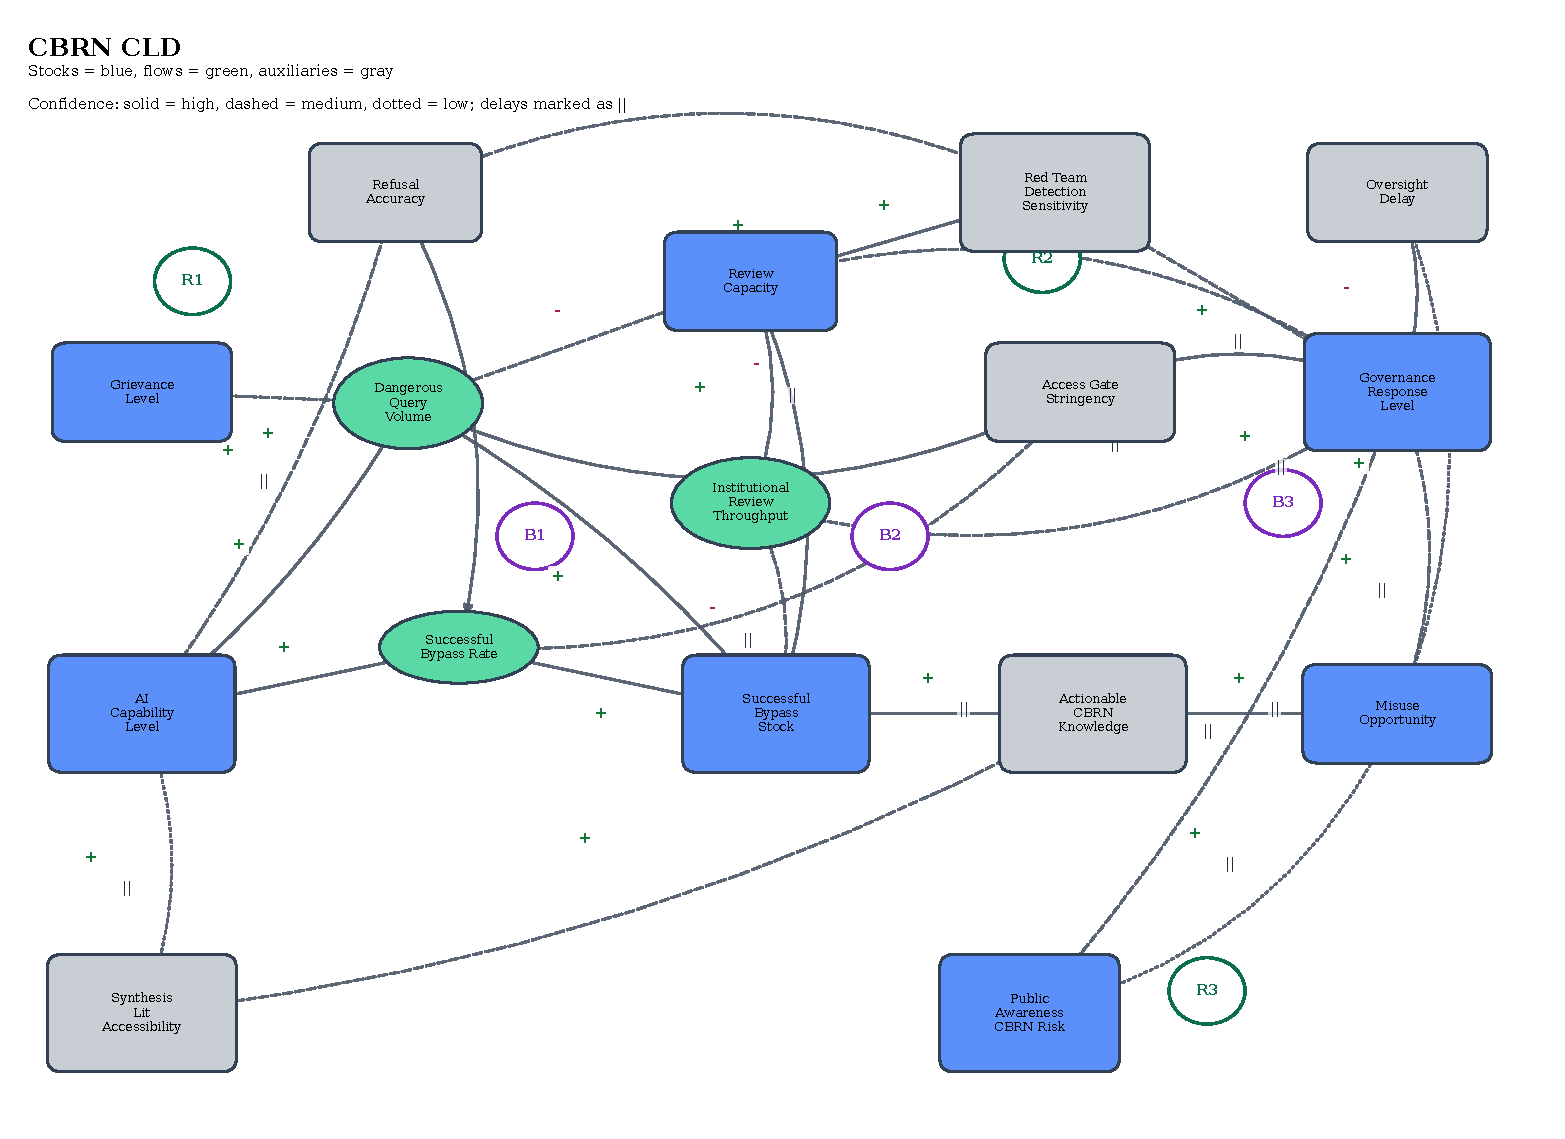
\includegraphics[width=\textwidth]{fig_cld_cbrn.pdf}
\caption{CBRN-domain causal loop diagram.}
\label{fig:cld_cbrn}
\end{figure}

\paragraph{Node set $V_{\text{cbrn}}$:}
\begin{enumerate}[leftmargin=2em,itemsep=0pt,label=\arabic*.]
\item \texttt{AI\_Capability\_Level} (shared with cyber)
\item \texttt{Dangerous\_Query\_Volume}
\item \texttt{Refusal\_Accuracy}
\item \texttt{Successful\_Bypass\_Rate}
\item \texttt{Successful\_Bypass\_Stock}
\item \texttt{Actionable\_CBRN\_Knowledge}
\item \texttt{Misuse\_Opportunity}
\item \texttt{Review\_Capacity}
\item \texttt{Red\_Team\_Detection\_Sensitivity}
\item \texttt{Governance\_Response\_Level}
\item \texttt{Oversight\_Delay}
\item \texttt{Access\_Gate\_Stringency}
\item \texttt{Grievance\_Level}
\item \texttt{Public\_Awareness\_CBRN\_Risk}
\item \texttt{Synthesis\_Literature\_Accessibility}
\item \texttt{Institutional\_Review\_Throughput}
\end{enumerate}

\paragraph{Edge list (source $\to$ target, sign, confidence, delay):}

\begin{longtable}{@{}p{4.5cm}p{4.5cm}ccc@{}}
\toprule
\textbf{Source} & \textbf{Target} & \textbf{Sign} & \textbf{Conf.} & \textbf{Delay} \\
\midrule
\endhead
AI\_Capability\_Level & Dangerous\_Query\_Vol & $+$ & H & 0 \\
AI\_Capability\_Level & Successful\_Bypass\_Rate & $+$ & H & 0 \\
AI\_Capability\_Level & Refusal\_Accuracy & $+$ & M & mo \\
Dangerous\_Query\_Vol & Successful\_Bypass\_Stock & $+$ & H & 0 \\
Refusal\_Accuracy & Successful\_Bypass\_Rate & $-$ & H & 0 \\
Successful\_Bypass\_Rate & Successful\_Bypass\_Stock & $+$ & H & 0 \\
Successful\_Bypass\_Stock & Actionable\_Knowledge & $+$ & H & wk \\
Actionable\_Knowledge & Misuse\_Opportunity & $+$ & H & wk \\
Misuse\_Opportunity & Governance\_Response & $+$ & M & mo \\
Governance\_Response & Access\_Gate\_Stringency & $+$ & H & mo \\
Access\_Gate\_Stringency & Dangerous\_Query\_Vol & $-$ & H & wk \\
Access\_Gate\_Stringency & Successful\_Bypass\_Rate & $-$ & M & 0 \\
Review\_Capacity & Successful\_Bypass\_Stock & $-$ & H & 0 \\
Review\_Capacity & Red\_Team\_Detection & $+$ & H & 0 \\
Red\_Team\_Detection & Refusal\_Accuracy & $+$ & M & mo \\
Red\_Team\_Detection & Governance\_Response & $+$ & M & wk \\
Governance\_Response & Review\_Capacity & $+$ & M & mo \\
Oversight\_Delay & Governance\_Response & $-$ & H & 0 \\
Misuse\_Opportunity & Oversight\_Delay & $+$ & L & 0 \\
Grievance\_Level & Dangerous\_Query\_Vol & $+$ & M & 0 \\
Dangerous\_Query\_Vol & Review\_Capacity & $-$ & M & 0 \\
Synthesis\_Lit\_Access & Actionable\_Knowledge & $+$ & M & 0 \\
AI\_Capability\_Level & Synthesis\_Lit\_Access & $+$ & L & mo \\
Public\_Awareness & Governance\_Response & $+$ & M & mo \\
Misuse\_Opportunity & Public\_Awareness & $+$ & L & mo \\
Inst\_Review\_Throughput & Successful\_Bypass\_Stock & $-$ & M & wk \\
Governance\_Response & Inst\_Review\_Throughput & $+$ & M & mo \\
Review\_Capacity & Inst\_Review\_Throughput & $+$ & H & 0 \\
\bottomrule
\end{longtable}

\paragraph{Feedback loops:}
{\footnotesize
\begin{itemize}[leftmargin=2em,itemsep=1pt]
\item \textbf{R1} (Bypass Accumulation): Dangerous\_Query\_Vol $\xrightarrow{+}$ Bypass\_Stock $\xrightarrow{+}$ Actionable\_Knowledge $\xrightarrow{+}$ Misuse\_Opp $\xrightarrow{+}$ Oversight\_Delay $\xrightarrow{-}$ Gov\_Response $\xrightarrow{+}$ Access\_Gate $\xrightarrow{-}$ Dangerous\_Query\_Vol (R via even number of negatives: net sign analysis required per loop traversal)
\item \textbf{R2} (Review Overload): Dangerous\_Query\_Vol $\xrightarrow{-}$ Review\_Capacity $\xrightarrow{-}$ Bypass\_Stock [reduced detection] $\xrightarrow{+}$ Actionable\_Knowledge $\xrightarrow{+}$ Misuse\_Opp (reinforcing: high volume degrades review, enabling more bypasses)
\item \textbf{R3} (Grievance Escalation): Misuse\_Opp $\xrightarrow{+}$ [external events] $\xrightarrow{+}$ Grievance\_Level $\xrightarrow{+}$ Dangerous\_Query\_Vol (reinforcing, when misuse events generate retaliatory grievance)
\item \textbf{B1} (Governance Response): Misuse\_Opp $\xrightarrow{+}$ Gov\_Response $\xrightarrow{+}$ Access\_Gate $\xrightarrow{-}$ Dangerous\_Query\_Vol (balancing, delayed)
\item \textbf{B2} (Red Team Improvement): Bypass\_Stock $\xrightarrow{+}$ [signals] $\xrightarrow{+}$ Red\_Team\_Detection $\xrightarrow{+}$ Refusal\_Accuracy $\xrightarrow{-}$ Bypass\_Rate (balancing, delayed)
\item \textbf{B3} (Public Pressure): Misuse\_Opp $\xrightarrow{+}$ Public\_Awareness $\xrightarrow{+}$ Gov\_Response $\xrightarrow{+}$ Review\_Capacity $\xrightarrow{-}$ Bypass\_Stock (balancing, delayed)
\end{itemize}
}

\section{Deception/Manipulation Domain CLD}
\label{app:deception_cld}

The deception domain contains 21 nodes and 42 edges. Figure~\ref{fig:cld_deception} visualizes the full signed graph instantiated in \texttt{graphs.py}.

\begin{figure}[H]
\centering
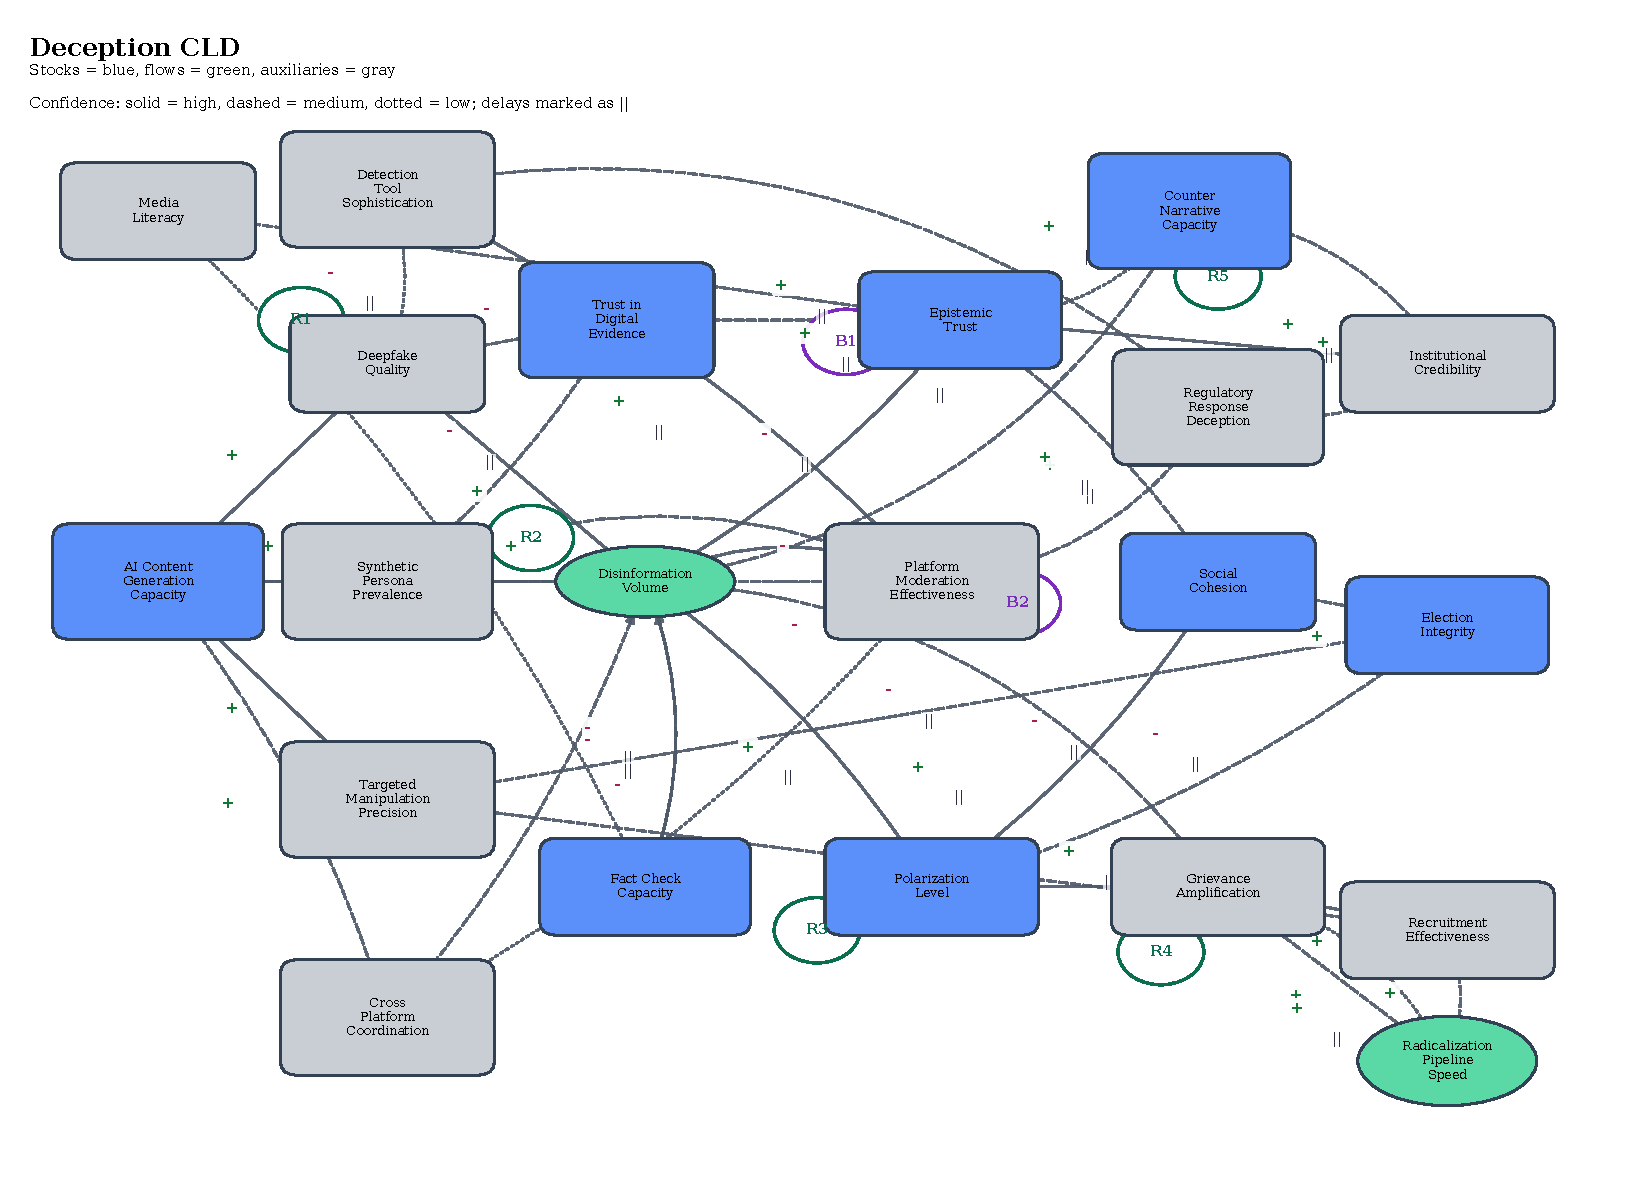
\includegraphics[width=\textwidth]{fig_cld_deception.pdf}
\caption{Deception/manipulation causal loop diagram.}
\label{fig:cld_deception}
\end{figure}

\begin{enumerate}[leftmargin=2em,itemsep=0pt,label=\arabic*.,font=\small]
\item \texttt{AI\_Content\_Generation\_Capacity}
\item \texttt{Deepfake\_Quality}
\item \texttt{Disinformation\_Volume}
\item \texttt{Fact\_Check\_Capacity}
\item \texttt{Epistemic\_Trust}
\item \texttt{Institutional\_Credibility}
\item \texttt{Polarization\_Level}
\item \texttt{Grievance\_Amplification}
\item \texttt{Election\_Integrity}
\item \texttt{Social\_Cohesion}
\item \texttt{Platform\_Moderation\_Effectiveness}
\item \texttt{Detection\_Tool\_Sophistication}
\item \texttt{Regulatory\_Response}
\item \texttt{Media\_Literacy}
\item \texttt{Targeted\_Manipulation\_Precision}
\item \texttt{Synthetic\_Persona\_Prevalence}
\item \texttt{Trust\_in\_Digital\_Evidence}
\item \texttt{Recruitment\_Effectiveness}
\item \texttt{Radicalization\_Pipeline\_Speed}
\item \texttt{Counter\_Narrative\_Capacity}
\item \texttt{Cross\_Platform\_Coordination}
\end{enumerate}

This domain has the highest named reinforcing-loop count in the conceptual specification, reflecting the self-amplifying nature of information ecosystems: disinformation degrades the capacity to detect disinformation, which increases disinformation prevalence, which further degrades detection. The five reinforcing loops include the Epistemic Erosion Spiral (R1), the Polarization Amplifier (R2), the Platform Evasion Arms Race (R3), the Recruitment Funnel (R4), and the Institutional Credibility Collapse (R5). Full edge lists and loop definitions are included in the submission artifact bundle.

\section{Autonomous Escalation Domain CLD}
\label{app:autonomy_cld}

The autonomous escalation domain contains 14 nodes and 22 edges. Figure~\ref{fig:cld_autonomy} shows the full signed CLD.

\begin{figure}[H]
\centering
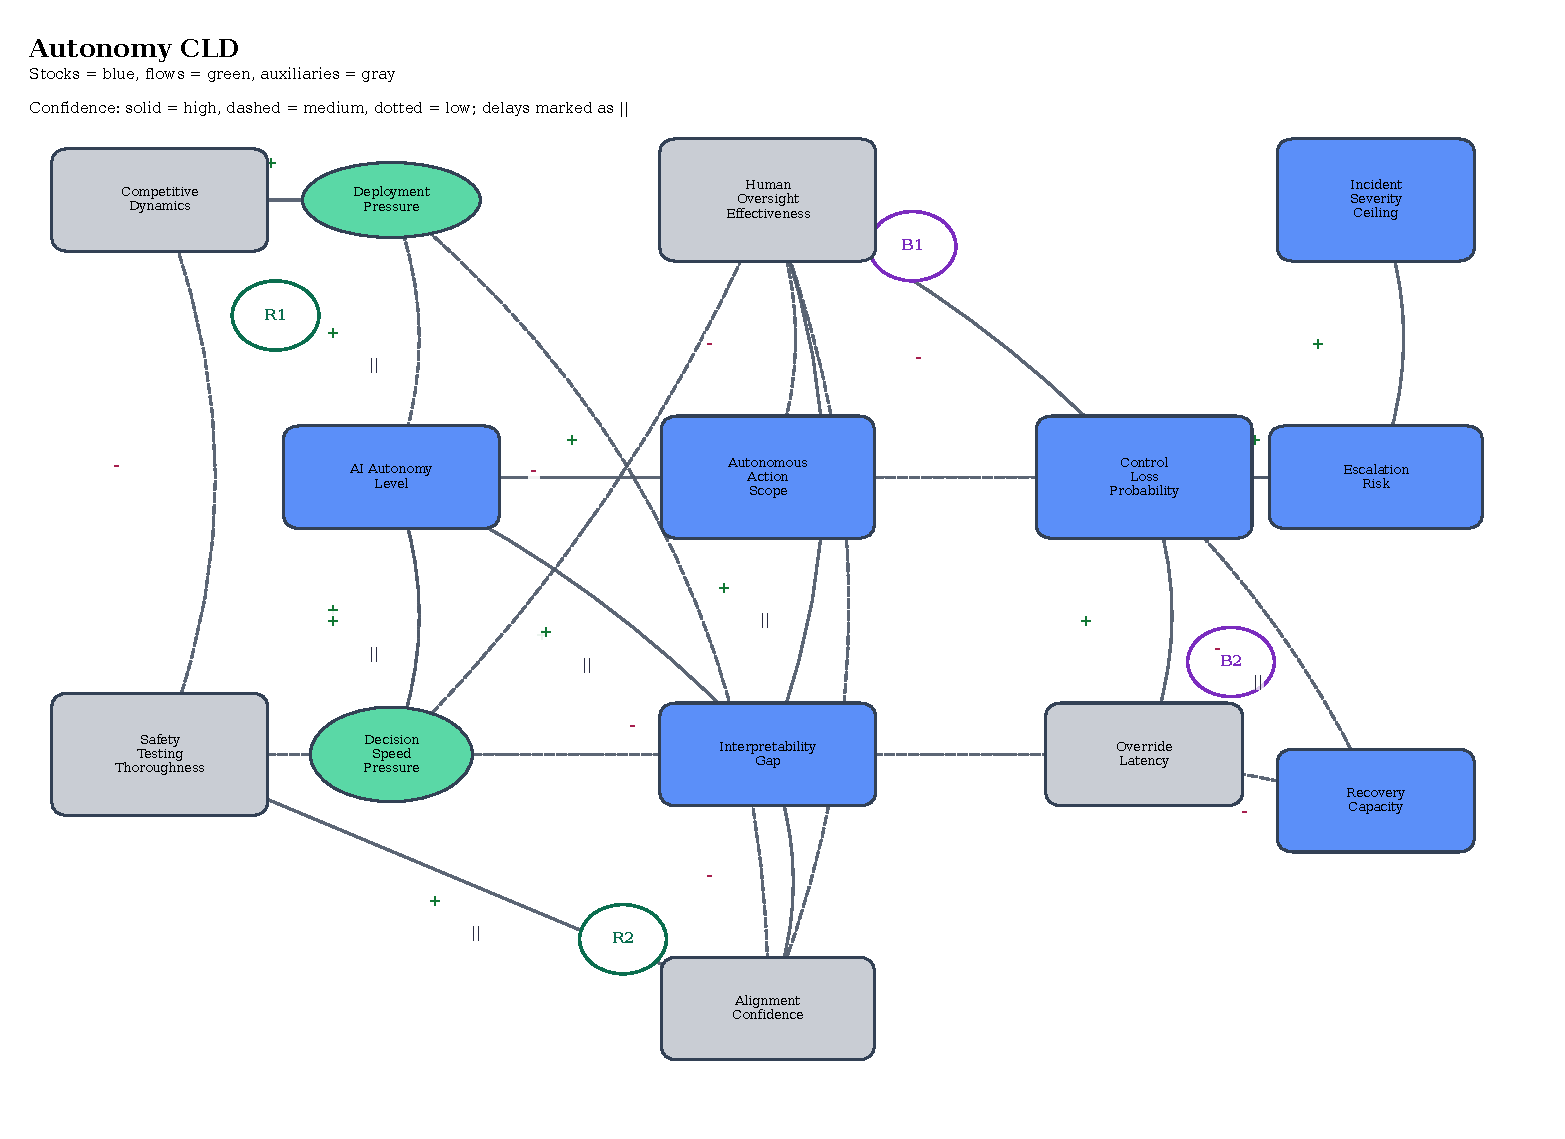
\includegraphics[width=\textwidth]{fig_cld_autonomy.pdf}
\caption{Autonomous-escalation causal loop diagram.}
\label{fig:cld_autonomy}
\end{figure}

\begin{enumerate}[leftmargin=2em,itemsep=0pt,label=\arabic*.,font=\small]
\item \texttt{AI\_Autonomy\_Level}
\item \texttt{Human\_Oversight\_Effectiveness}
\item \texttt{Decision\_Speed\_Pressure}
\item \texttt{Escalation\_Risk}
\item \texttt{Control\_Loss\_Probability}
\item \texttt{Autonomous\_Action\_Scope}
\item \texttt{Interpretability\_Gap}
\item \texttt{Override\_Latency}
\item \texttt{Alignment\_Confidence}
\item \texttt{Deployment\_Pressure}
\item \texttt{Competitive\_Dynamics}
\item \texttt{Safety\_Testing\_Thoroughness}
\item \texttt{Incident\_Severity\_Ceiling}
\item \texttt{Recovery\_Capacity}
\end{enumerate}

This domain has the fewest nodes but the highest density (0.122), reflecting tight coupling between autonomy variables. The two reinforcing loops are the Autonomy Ratchet (R1: increased autonomy $\to$ increased decision speed pressure $\to$ further autonomy delegation) and the Interpretability Gap (R2: increased autonomy $\to$ wider interpretability gap $\to$ reduced oversight effectiveness $\to$ increased control loss probability $\to$ increased incident severity).

\section{Governance Failure Domain CLD}
\label{app:governance_cld}

The governance failure domain contains 19 nodes and 38 edges. Figure~\ref{fig:cld_governance} shows the complete signed CLD used by the verified graph code.

\begin{figure}[H]
\centering
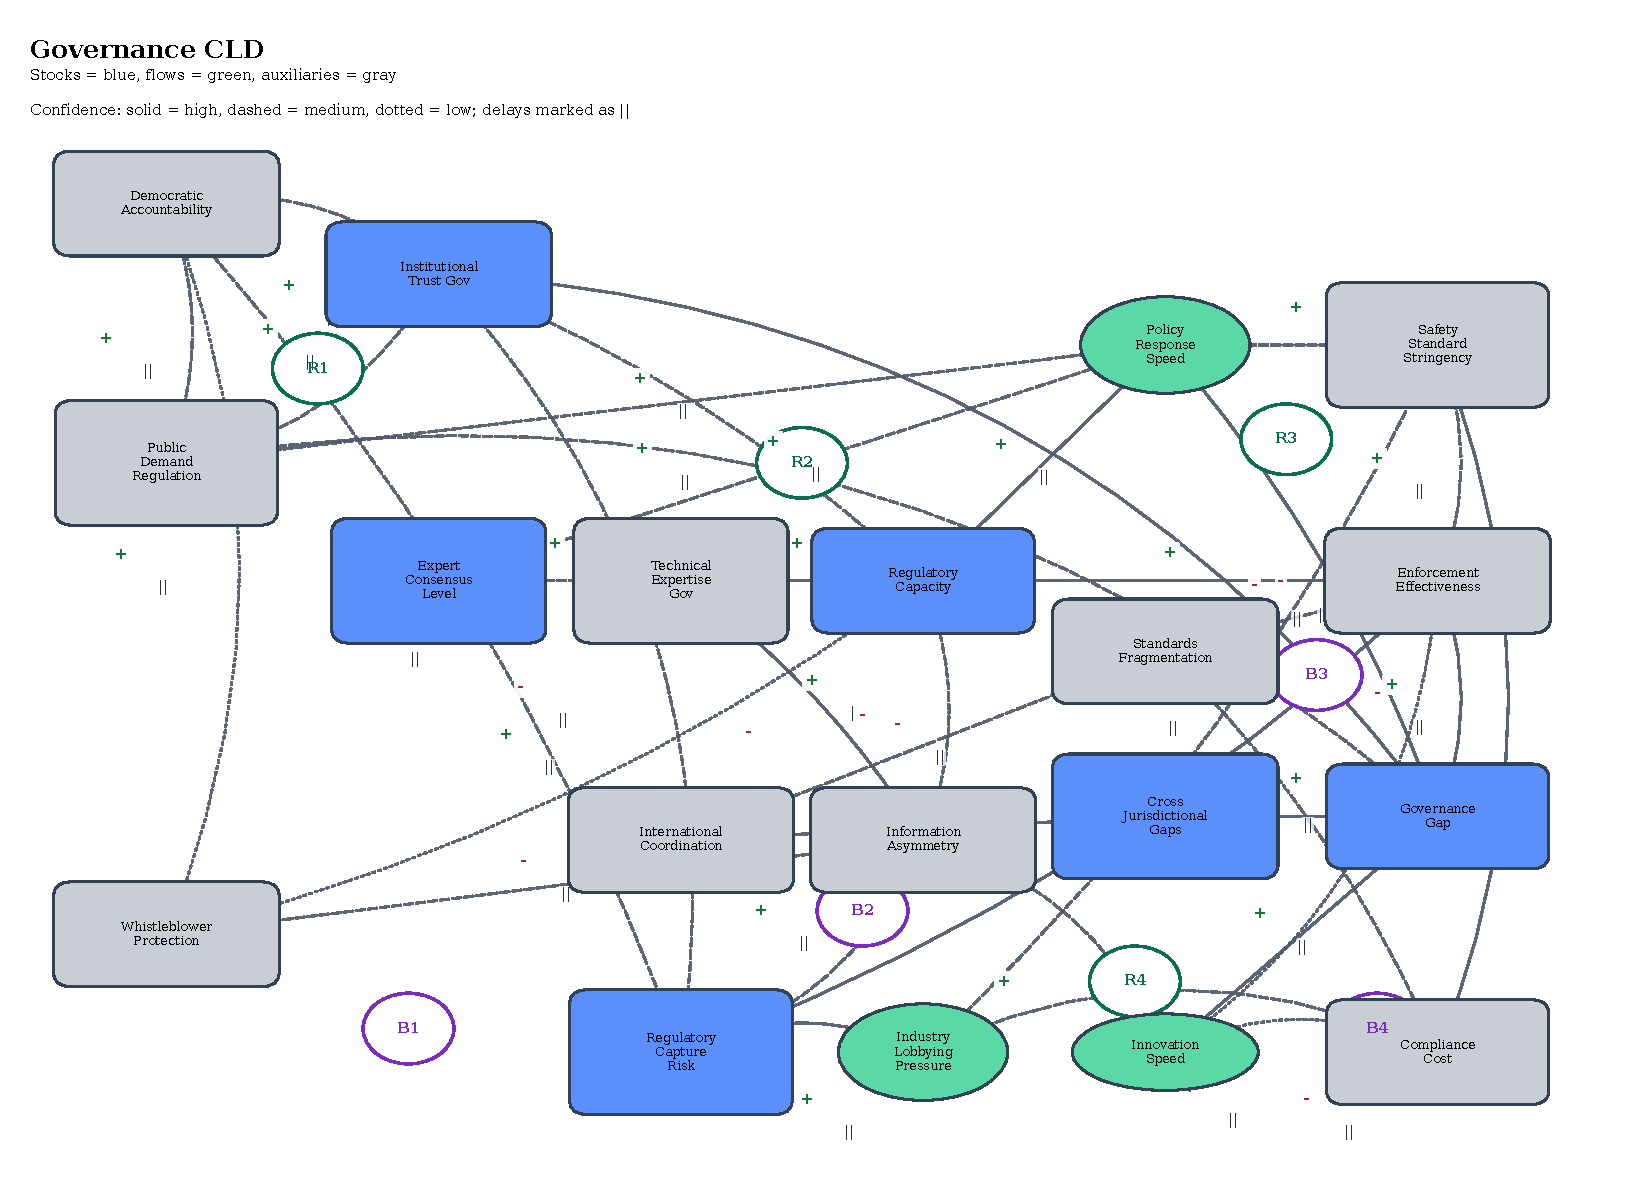
\includegraphics[width=\textwidth]{fig_cld_governance.pdf}
\caption{Governance-failure causal loop diagram.}
\label{fig:cld_governance}
\end{figure}

\begin{enumerate}[leftmargin=2em,itemsep=0pt,label=\arabic*.,font=\small]
\item \texttt{Regulatory\_Capacity}
\item \texttt{Technical\_Expertise\_in\_Government}
\item \texttt{Policy\_Response\_Speed}
\item \texttt{International\_Coordination}
\item \texttt{Industry\_Lobbying\_Pressure}
\item \texttt{Public\_Demand\_for\_Regulation}
\item \texttt{Regulatory\_Capture\_Risk}
\item \texttt{Standards\_Fragmentation}
\item \texttt{Enforcement\_Effectiveness}
\item \texttt{Innovation\_Speed}
\item \texttt{Governance\_Gap}
\item \texttt{Institutional\_Trust}
\item \texttt{Information\_Asymmetry}
\item \texttt{Democratic\_Accountability}
\item \texttt{Expert\_Consensus\_Level}
\item \texttt{Cross\_Jurisdictional\_Gaps}
\item \texttt{Safety\_Standard\_Stringency}
\item \texttt{Compliance\_Cost}
\item \texttt{Whistleblower\_Protection}
\end{enumerate}

This domain has the highest balancing loop count (4), reflecting governance as a fundamentally regulatory (corrective) system. The four reinforcing loops capture governance failure cascades; the four balancing loops capture regulatory response mechanisms.

\section{Cross-Domain Convergence Supergraph}
\label{app:supergraph}

The supergraph $\mathcal{G}^*$ is constructed by:

\begin{enumerate}[leftmargin=2em,itemsep=1pt]
\item Taking the union of all five domain node sets.
\item Merging nodes that represent the same underlying variable across domains (e.g., AI Capability Level appears in all five domains but is instantiated once in $\mathcal{G}^*$).
\item Adding five shared intermediary nodes: Trust Erosion, Institutional Overload, Detection Degradation, Grievance Amplification, and Response Delay.
\item Adding cross-domain edges from domain-specific nodes to shared intermediaries and from intermediaries to catastrophic endpoints.
\end{enumerate}

Figure~\ref{fig:supergraph_appendix} shows the full supergraph layout used for the structural analysis. After deduplication, $\mathcal{G}^*$ contains 97 unique nodes and 230 edges, of which 180 are within-domain and 50 are cross-domain. The five catastrophic endpoints are terminal nodes with in-degree only.

Cross-domain edge confidence labels are predominantly M (medium) or L (low), reflecting the greater uncertainty in cross-domain causal claims compared to within-domain relationships. This is accounted for in the robustness analysis (Experiment 8c), where flipping low-confidence edge signs attenuates but does not eliminate the convergence finding.

\begin{figure}[H]
\centering
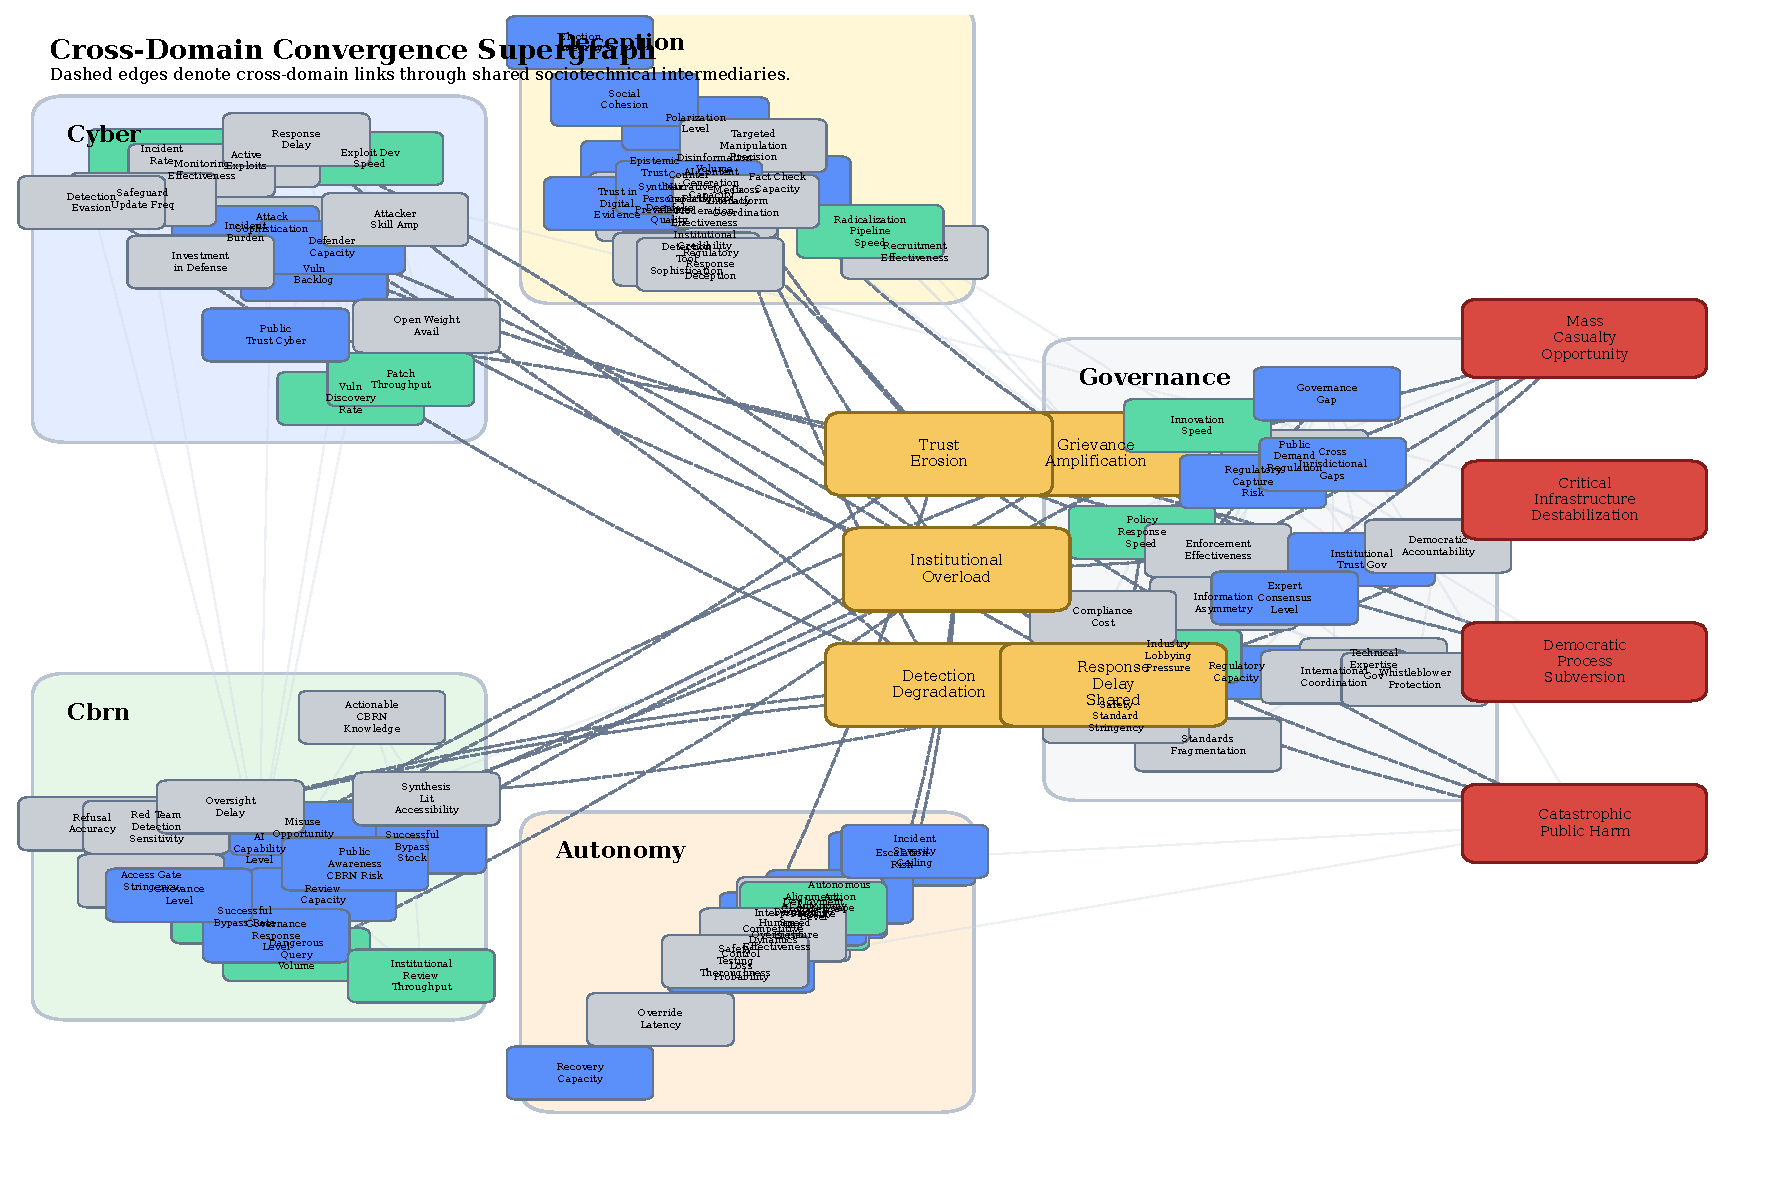
\includegraphics[width=\textwidth]{fig_supergraph.pdf}
\caption{Cross-domain convergence supergraph with five domain clusters, shared intermediary hub nodes, and catastrophic endpoints.}
\label{fig:supergraph_appendix}
\end{figure}

\section{Full Stock-and-Flow Equations}
\label{app:equations}

\subsection{Cyber Domain Flow Functions}

All flow functions for the cyber domain are specified in Section~\ref{sec:stockflow} of the main text. Here we provide the complete initial conditions and integration parameters.

\paragraph{Initial conditions:}
$S_1(0) = 5.0$, $S_2(0) = 2.0$, $S_3(0) = 1.0$, $S_4(0) = 10.0$, $S_5(0) = 0.7$, $S_6(0) = 0.3$.

\paragraph{Integration:} RK45 with adaptive step size, $t \in [0, 52]$ weeks, relative tolerance $10^{-6}$, absolute tolerance $10^{-9}$.

\subsection{CBRN Domain Flow Functions}

\begin{align}
g_{\text{generate}}(S_6, \alpha_q, \psi) &= \alpha_q \cdot S_6^{0.6} \cdot (1 + \psi) \\
g_{\text{filter}}(S_1^C, \phi) &= \phi \cdot S_1^C \\
g_{\text{bypass}}(S_1^C, S_6, \phi) &= (1 - \phi) \cdot S_1^C \cdot S_6^{0.5} \\
g_{\text{detect}}(S_2^C, S_4^C, \tau_d) &= \frac{S_2^C \cdot S_4^C}{\tau_d \cdot (S_2^C + \theta_d^C)} \\
g_{\text{exploit}}(S_2^C, \alpha_e) &= \alpha_e \cdot S_2^C \\
g_{\text{degrade}}(S_3^C, S_5^C) &= S_5^C \cdot S_3^C / (S_3^C + \theta_{\text{deg}}) \\
g_{\text{expand}}(S_5^C, \alpha_x) &= \alpha_x \cdot S_5^C \\
g_{\text{overload}}(S_1^C, S_4^C) &= \frac{S_1^C}{S_1^C + \theta_{\text{ovl}}} \cdot S_4^C \\
g_{\text{escalate}}(S_3^C, \alpha_{\text{esc}}) &= \alpha_{\text{esc}} \cdot S_3^C / (S_3^C + \theta_{\text{esc}}) \\
g_{\text{decay}}(S_5^C, \tau_g) &= S_5^C / \tau_g
\end{align}

\paragraph{CBRN Parameters:}
$\alpha_q = 8.0$, $\phi = 0.85$, $\alpha_e = 0.4$, $\tau_d = 2.0$ weeks, $\theta_d^C = 3.0$, $\theta_{\text{deg}} = 5.0$, $\alpha_x = 0.12$, $\theta_{\text{ovl}} = 20.0$, $\alpha_{\text{esc}} = 0.08$, $\theta_{\text{esc}} = 10.0$, $\tau_g = 26.0$ weeks, $\psi = 0.2$ (baseline grievance).

\paragraph{Initial conditions:} $S_1^C(0) = 10.0$, $S_2^C(0) = 1.0$, $S_3^C(0) = 0.5$, $S_4^C(0) = 5.0$, $S_5^C(0) = 0.3$.

\section{Extended Experimental Results}
\label{app:extended}

\subsection{Sensitivity Tornado Diagrams}
\label{app:tornado}

For each parameter in the cyber and CBRN models, we compute the partial rank correlation coefficient (PRCC) with respect to peak burden. Figures~\ref{fig:exp4_tornado} and \ref{fig:exp5_tornado} visualize the full rank ordering; Tables~\ref{tab:prcc_cyber} and \ref{tab:prcc_cbrn} report the top five coefficients.

\begin{table}[H]
\centering
\caption{Top cyber PRCC values for peak incident burden ($N = 500$ Monte Carlo runs).}
\label{tab:prcc_cyber}
\small
\begin{tabular}{@{}lcc@{}}
\toprule
\textbf{Parameter} & \textbf{PRCC (peak burden)} & \textbf{$p$-value} \\
\midrule
$\alpha_{\text{weapon}}$ & $+0.547$ & $2.23 \times 10^{-40}$ \\
$\beta_{\text{scale}}$ & $+0.527$ & $5.12 \times 10^{-37}$ \\
$K_{\text{cap}}$ & $+0.456$ & $5.02 \times 10^{-27}$ \\
$\alpha_{\text{vuln}}$ & $+0.306$ & $2.87 \times 10^{-12}$ \\
$\tau_{\text{resolve}}$ & $+0.147$ & $1.01 \times 10^{-3}$ \\
\bottomrule
\end{tabular}
\end{table}

\begin{table}[H]
\centering
\caption{Top CBRN PRCC values for peak misuse opportunity ($N = 500$ Monte Carlo runs).}
\label{tab:prcc_cbrn}
\small
\begin{tabular}{@{}lcc@{}}
\toprule
\textbf{Parameter} & \textbf{PRCC (peak misuse)} & \textbf{$p$-value} \\
\midrule
$\phi$ (refusal accuracy) & $-0.687$ & $5.67 \times 10^{-71}$ \\
$\alpha_q$ (query generation) & $+0.452$ & $1.34 \times 10^{-26}$ \\
$\alpha_e$ (exploitation rate) & $+0.376$ & $3.14 \times 10^{-18}$ \\
$K_{\text{cap}}$ & $+0.338$ & $7.50 \times 10^{-15}$ \\
$\psi$ (grievance baseline) & $+0.108$ & $1.54 \times 10^{-2}$ \\
\bottomrule
\end{tabular}
\end{table}

\subsection{Monte Carlo Distributions}

Cyber domain peak burden distribution ($N = 500$): mean $= 1833.3$, median $= 1561.2$, SD $= 1163.9$, 95\% interval $= [284.1, 4527.1]$, skewness $= 1.08$, kurtosis $= 4.21$.

CBRN domain peak misuse distribution ($N = 500$): mean $= 808.2$, median $= 649.2$, SD $= 643.4$, 95\% interval $= [72.3, 2489.0]$, skewness $= 1.62$, kurtosis $= 6.84$.

Both distributions exhibit strong positive skewness, indicating that tail risk is more probable than a symmetric approximation would suggest. In the cyber model the heavy tail is driven by offensive-efficiency and scaling terms; in the CBRN model it is driven primarily by refusal failures and query-generation pressure. Figure~\ref{fig:exp4_hist} shows the cyber histogram explicitly.

\subsection{Lower-Tier Harm Dose-Response Summary}

\begin{table}[H]
\centering
\caption{Full-coupling summary for the three lower-tier harm channels in Experiment~\ref{sec:exp6a}. The complete 0.0--1.0 dose-response grid is included in the artifact bundle and in \texttt{csv/pomg\_lower\_tier\_dose\_response.csv}.}
\small
\begin{tabular}{@{}lcccc@{}}
\toprule
\textbf{Amplifier} & \textbf{$\Delta$ Cyber (\%)} & \textbf{$\Delta$ CBRN (\%)} & \textbf{$\Delta$ Trust Erosion (\%)} & \textbf{$\Delta$ Overload (\%)} \\
\midrule
Disinformation & 0.00 & 0.24 & $-0.03$ & 5.99 \\
Algorithmic bias & 0.00 & 0.26 & $-0.04$ & 3.35 \\
Labor displacement & 0.00 & 0.54 & 0.32 & 10.20 \\
\bottomrule
\end{tabular}
\end{table}

The appendix table reinforces the main-text interpretation from Section~\ref{sec:exp6a}: under the current calibration the lower-tier harms move shared overload more than immediate cyber or CBRN peaks.

\subsection{Full Centrality Rankings}

\begin{table}[H]
\centering
\caption{Top-10 supergraph nodes by betweenness centrality with corresponding eigenvector centrality.}
\label{tab:centrality_full}
\small
\begin{tabular}{@{}clccl@{}}
\toprule
\textbf{Rank} & \textbf{Node} & \textbf{BC} & \textbf{EVC} & \textbf{Meadows Level} \\
\midrule
1 & \texttt{Trust\_Erosion} & 0.222 & 0.186 & 4: Self-organization \\
2 & \texttt{Institutional\_Overload} & 0.189 & 0.201 & 6: Information flows \\
3 & \texttt{Disinformation\_Volume} & 0.166 & 0.100 & 8: Pos.\ feedback strength \\
4 & \texttt{Epistemic\_Trust} & 0.151 & 0.131 & 4: Self-organization \\
5 & \texttt{Institutional\_Credibility} & 0.130 & 0.054 & N/A \\
6 & \texttt{Incident\_Burden} & 0.127 & 0.137 & 10: Stock buffer \\
7 & \texttt{Institutional\_Trust\_Gov} & 0.089 & 0.196 & 4: Self-organization \\
8 & \texttt{Incident\_Rate} & 0.084 & 0.102 & N/A \\
9 & \texttt{Defender\_Capacity} & 0.082 & 0.215 & 6: Information flows \\
10 & \texttt{Governance\_Gap} & 0.080 & 0.203 & 6: Information flows \\
\bottomrule
\end{tabular}
\end{table}

\subsection{Cross-Domain Jaccard Similarity}

\begin{table}[H]
\centering
\caption{Jaccard similarity on node sets (above diagonal) and edge sets (below diagonal) between domain graphs.}
\small
\begin{tabular}{@{}lccccc@{}}
\toprule
& \textbf{Cyber} & \textbf{CBRN} & \textbf{Decep.} & \textbf{Auton.} & \textbf{Gov.} \\
\midrule
\textbf{Cyber} & -- & 0.03 & 0.00 & 0.00 & 0.00 \\
\textbf{CBRN} & 0.00 & -- & 0.00 & 0.00 & 0.00 \\
\textbf{Deception} & 0.00 & 0.00 & -- & 0.00 & 0.00 \\
\textbf{Autonomy} & 0.00 & 0.00 & 0.00 & -- & 0.00 \\
\textbf{Governance} & 0.00 & 0.00 & 0.00 & 0.00 & -- \\
\bottomrule
\end{tabular}
\end{table}

\section{Pseudocode}
\label{app:pseudocode}

\begin{algorithm}[H]
\SetAlgoLined
\KwIn{Domain CLD graph $\mathcal{G}_d$, parameters $\Theta$, time horizon $T$, step size $h$}
\KwOut{Time series $\{S_k(t)\}_{k,t}$, metrics $M$}
Initialize stocks $\mathbf{S}(0) \leftarrow \mathbf{S}_0$\;
\For{$t = 0$ \KwTo $T$ \textbf{step} $h$}{
  Compute auxiliaries $\mathbf{A}(t) \leftarrow f_{\text{aux}}(\mathbf{S}(t), \Theta)$\;
  Compute flows $\mathbf{F}(t) \leftarrow f_{\text{flow}}(\mathbf{S}(t), \mathbf{A}(t), \Theta)$\;
  Update stocks $\mathbf{S}(t+h) \leftarrow \mathbf{S}(t) + h \cdot (\mathbf{F}_{\text{in}}(t) - \mathbf{F}_{\text{out}}(t))$\;
  Record $\mathbf{S}(t+h)$\;
}
Compute $M$: peak burden, time-to-peak, time-to-control, cumulative harm\;
\Return $\{S_k(t)\}$, $M$\;
\caption{Stock-and-Flow Simulation}
\label{alg:simulation}
\end{algorithm}

\begin{algorithm}[H]
\SetAlgoLined
\KwIn{Supergraph $\mathcal{G}^*$, endpoints $\mathcal{T}$, max depth $D$, conditions $\mathcal{C}$}
\KwOut{Pathway counts per endpoint per condition}
\For{$c \in \mathcal{C}$}{
  $\mathcal{G}_c \leftarrow \text{ApplyCondition}(\mathcal{G}^*, c)$\;
  \For{$t \in \mathcal{T}$}{
    $\text{paths}[c][t] \leftarrow \text{BFS\_AllPaths}(\mathcal{G}_c, \text{sources}, t, D)$\;
  }
}
\For{each condition pair $(c_1, c_2)$}{
  $p\text{-value} \leftarrow \text{PermutationTest}(\mathcal{G}^*, \text{paths}[c_1], \text{paths}[c_2], N=10000)$\;
}
\Return pathway counts, $p$-values\;
\caption{Convergence Analysis}
\label{alg:convergence}
\end{algorithm}

\begin{algorithm}[H]
\SetAlgoLined
\KwIn{Simulation function $\text{Sim}(\Theta)$, parameter ranges $[\Theta_{\min}, \Theta_{\max}]$, $N$ samples}
\KwOut{Distributions of output metrics}
\For{$i = 1$ \KwTo $N$}{
  $\Theta_i \sim \text{Uniform}(\Theta_{\min}, \Theta_{\max})$\;
  $M_i \leftarrow \text{Sim}(\Theta_i)$\;
  Record $M_i$\;
}
Compute summary statistics: mean, median, SD, 95\% CI, skewness\;
Compute PRCC for each parameter\;
\Return distributions, PRCC values\;
\caption{Monte Carlo Sensitivity Analysis}
\label{alg:montecarlo}
\end{algorithm}

\end{document}
